% This is part of Mes notes de mathématique
% Copyright (c) 2006-2015
%   Laurent Claessens, Carlotta Donadello
% See the file fdl-1.3.txt for copying conditions.
 
%+++++++++++++++++++++++++++++++++++++++++++++++++++++++++++++++++++++++++++++++++++++++++++++++++++++++++++++++++++++++++++
\section{Dérivée directionnelle de fonctions composées}		\label{SecDerDirFnComp}
%+++++++++++++++++++++++++++++++++++++++++++++++++++++++++++++++++++++++++++++++++++++++++++++++++++++++++++++++++++++++++++

Étant donné que nous allons voir en détail la différentielle de fonctions composées à la proposition \ref{PropDiffCompose}, nous n'allons pas rentrer dans tous les détail ici.

Nous savons déjà comment dériver les fonctions composées de $\eR$ dans $\eR$. Si nous avons deux fonctions $f\colon \eR\to \eR$ et $u\colon \eR\to \eR$, nous formons la composée $\varphi=f\circ u\colon \eR\to \eR$ dont la dérivée vaut
\begin{equation}
	\varphi'(a)=f'\big( u(a) \big)u'(a).
\end{equation}


Considérons maintenant le cas un peu plus compliqué des fonctions $f\colon \eR\to \eR$ et $u\colon \eR^2\to \eR$, et de la composée
\begin{equation}
	\begin{aligned}
		\varphi\colon \eR^2&\to \eR \\
		\varphi(x,y)&= f\big( u(x,y) \big). 
	\end{aligned}
\end{equation}
Afin de calculer la dérivée partielle de $\varphi$ par rapport à $x$, nous admettons que pour tout $a$, $b$ et $t$, il existe $c\in\mathopen[ a , a+t \mathclose]$ tel que
\begin{equation}
	u(a+t,b)=u(a,b)+t\frac{ \partial u }{ \partial x }(c,b).
\end{equation}
Cela est une généralisation immédiate du théorème \ref{ThoAccFinis}. Nous devons calculer
\begin{equation}		\label{EqPremPasDiffxvp}
	\frac{ \partial \varphi }{ \partial x }(a,b)=\lim_{t\to 0} \frac{ \varphi(a+t,b)-\varphi(a,b) }{ t }=\lim_{t\to 0} \frac{ f\big( u(a+t,b) \big)-g\big( u(a,b) \big) }{ t }.
\end{equation}
Étant donné l'hypothèse que nous avons faite sur $u$, nous avons
\begin{equation}
	f\big( u(a+t,b) \big)=f\big( u(a,b)+t\frac{ \partial u }{ \partial x }(c,b) \big).
\end{equation}
En utilisant le théorème des accroissements finis pour $f$, nous avons un point $d$ entre $u(a,b)$ et $u(a,b)+t\frac{ \partial u }{ \partial x }(c,b)$ tel que
\begin{equation}
	f\big( u(a,b)+t\frac{ \partial u }{ \partial x }(c,b) \big)=f\big( u(a,b) \big)+t\frac{ \partial u }{ \partial x }(c,b)f'(d).
\end{equation}
Le numérateur de \eqref{EqPremPasDiffxvp} devient donc
\begin{equation}
	t\frac{ \partial u }{ \partial x }(c,b)f'(d).
\end{equation}
Certes les points $c$ et $d$ sont inconnus, mais nous savons que $c$ est entre $a$ et $a+t$ ainsi que $d$ se situe entre $u(a,b)$ et $u(a,b)+t\frac{ \partial u }{ \partial x }(c,b)$. Lorsque nous prenons la limite $t\to 0$, nous avons donc $\lim_{t\to 0} c=a$ et $\lim_{t\to 0} d=u(a,b)$. Nous avons alors
\begin{equation}
	\lim_{t\to 0} \frac{ t\frac{ \partial u }{ \partial x }(c,b)f'(d) }{ t }=\frac{ \partial u }{ \partial x }(a,b)f'\big( u(a,b) \big).
\end{equation}
La formule que nous avons obtenue (de façon pas très rigoureuse) est
\begin{equation}
	\frac{ \partial  }{ \partial x }f\big( u(x,y) \big)=\frac{ \partial u }{ \partial x }(x,y)f'\big( u(x,y) \big).
\end{equation}

Prenons maintenant un cas un peu plus compliqué où nous voudrions savoir les dérivées partielles de la fonction $\varphi$ donnée par
\begin{equation}
	\varphi(x,y,z)=f\big( u(x,y),v(x,y,z) \big)
\end{equation}
où $f\colon \eR^2\to \eR$, $u\colon \eR^2\to \eR$ et $v\colon \eR^3\to \eR$. 

Commençons par la dérivée partielles par rapport à $z$. Étant donné que $\varphi$ ne dépend de $z$ que via la seconde entrée de $f$, il est normal que seule la dérivée partielle de $f$ par rapport à sa seconde entrée arrive dans la formule :
\begin{equation}
	\frac{ \partial \varphi }{ \partial z }(x,y,z)=\frac{ \partial f }{ \partial v }\big( u(x,y),v(x,y,z) \big)\frac{ \partial v }{ \partial z }(x,y,z).
\end{equation}
La dérivée partielle par rapport à $y$ demande de tenir compte en même temps de la façon dont $f$ varie avec sa première entrée et la façon dont elle varie avec sa seconde entrée; cela nous fait deux termes :
\begin{equation}
	\frac{ \partial \varphi }{ \partial y }(x,y,z)=\frac{ \partial f }{ \partial u }\big( u(x,y),v(x,y,z) \big)\frac{ \partial u }{ \partial y }(x,y)+\frac{ \partial f }{ \partial v }\big( u(x,y),v(x,y,z) \big)\frac{ \partial v }{ \partial y }(x,y,z).
\end{equation}


Cette formule a une interprétation simple. Lançons un caillou du sommet d'une falaise. Son mouvement est une chute libre avec une vitesse initiale horizontale :
\begin{subequations}
	\begin{numcases}{}
		x(t)=v_0t\\
		y(t)=h_0-\frac{ gt^2 }{ 2 }
	\end{numcases}
\end{subequations}
où $v_0$ est la vitesse initiale horizontale et $h_0$ est la hauteur de la falaise. Si nous sommes intéressés à la distance entre le caillou et le bas de la falaise (point $(0,0)$), le théorème de Pythagore nous dit que
\begin{equation}
	d(t)=\sqrt{x^2(t),y^2(t)}.
\end{equation}
Pour trouver la variation de la distance par rapport au temps il faut savoir de combien la distance varie lorsque $x$ varie et multiplier par la variation de $x$ par rapport à $t$, et puis faire la même chose avec $y$.

\begin{theorem}		\label{ThoDerDirFnComp}
	Soit $g\colon \eR^m\to \eR^n$ une fonction différentiable en $a$, et $f\colon \eR^n\to \eR^p$ une fonction différentiable en $g(a)$. Si nous définissons $\varphi(x)=(f\circ g)(x)$, alors pour tout $i=1,\ldots,m$, nous avons
	\begin{equation}
		\frac{ \partial \varphi }{ \partial x_i }(a)=\sum_{k=1}^n\frac{ \partial f }{ \partial y_k }\big( g(a) \big)\frac{ \partial g }{ \partial x_i }
	\end{equation}
	où $\frac{ \partial f }{ \partial y_k }$ dénote la dérivée partielle de $f$ par rapport à sa $k$-ième variable.
\end{theorem}

Donnons un exemple d'utilisation de cette formule. Si
\begin{equation}
	\begin{aligned}[]
		g\colon \eR^2\to \eR^3\\
		f\colon \eR^3\to \eR,
	\end{aligned}
\end{equation}
nous avons $\varphi\colon \eR^2\to \eR$. Les dérivées partielles de $\varphi$ sont données par les formules
\begin{equation}
	\frac{ \partial \varphi }{ \partial x }(x,y)=\frac{ \partial f }{ \partial x_1 }\big( g(x,y) \big)\frac{ \partial g_1 }{ \partial x }(x,y)+\frac{ \partial f }{ \partial x_2 }\big( g(x,y) \big)\frac{ \partial g_2 }{ \partial y }(x,y)+\frac{ \partial f }{ \partial x_3 }\big( g(x,y) \big)\frac{ \partial g_3 }{ \partial x }(x,y)
\end{equation}
et
\begin{equation}
	\frac{ \partial \varphi }{ \partial y }(x,y)=\frac{ \partial f }{ \partial x_1 }\big( g(x,y) \big)\frac{ \partial g_1 }{ \partial y }(x,y)+\frac{ \partial f }{ \partial x_2 }\big( g(x,y) \big)\frac{ \partial g_2 }{ \partial y }(x,y)+\frac{ \partial f }{ \partial x_3 }\big( g(x,y) \big)\frac{ \partial g_3 }{ \partial y }(x,y)
\end{equation}
Notez que les dérivées de $\varphi$ et des composantes de $g$ sont calculées en $(x,y)$, tandis que celles de $f$ sont calculées en $g(x,y)$.

%++++++++++++++++++++++++++++++++++++++++++++++++++++++++++++++++++++++++++++++++++++++++++++++++++++++++++++++++++++++
\section{Théorèmes des accroissements finis}		\label{SecThoAccrsFinis}
%++++++++++++++++++++++++++++++++++++++++++++++++++++++++++++++++++++++++++++++++++++++++++++++++++++++++++++++++++++++

Nous avons déjà démontré (lemme \ref{LemdfaSurLesPartielles}) que si $f$ est différentiable au point $x$ alors  $df_x(u)=\partial_uf(x)$. Une importante conséquence est le théorème des accroissements finis
\begin{theorem}[Accroissements finis, inégalité de la moyenne]\label{val_medio_2}
   Soit $U$ un ouvert dans $\eR^m$ et soit $f:U\to\eR^n$ une fonction différentiable. Soient $a$ et $b$ deux point dans $U$, $a\neq b$, tels que le segment $[a,b]$ soit contenu dans $U$. Alors
   \begin{equation}
        \|f(b)-f(a)\|_n\leq \sup_{x\in[a,b]}\|df(x)\|_{\mathcal{L}(\eR^m,\eR^n)}\|b-a\|_m.
   \end{equation}
\end{theorem}
\index{application!différentiable}
\index{inégalité!de la moyenne}
\index{théorème!accroissements finis!forme générale}
Dans le cas de dimension infinie, il y a le théorème \ref{ThoNAKKght}.

\begin{proof}
 On utilise le théorème \ref{val_medio_1} et le fait que 
\[
\|\partial_u f(x)\|_n\leq \|df(x)\|_{\mathcal{L}(\eR^m,\eR^n)}\|u\|_m,
\]
pour tout $u$ dans $\eR^m$.
\end{proof}

La proposition suivante est une application fondamentale du théorème des accroissements finis \ref{val_medio_2}.
\begin{proposition}		\label{PropAnnulationEtConstance}
	Soit $U$ un ouvert connexe par arcs de $\eR^m$ et une fonction $f\colon U\to \eR^n$. Les conditions suivantes sont équivalentes :
	\begin{enumerate}
		\item\label{ItemPropCstDiffZeroi}
			$f$ est constante;
		\item\label{ItemPropCstDiffZeroii}
			$f$ est différentiable et $df(a)=0$ pour tout $a\in U$;
		\item\label{ItemPropCstDiffZeroiii}
			les dérivées partielles $\partial_1f,\ldots,\partial_mf$ existent et sont nulles sur $U$.
	\end{enumerate}
\end{proposition}
\index{connexité!par arc!fonction différentiable}
\index{différentiabilité}

\begin{proof}
	Nous allons démonter les équivalences en plusieurs étapes. D'abord \ref{ItemPropCstDiffZeroi} $\Rightarrow$ \ref{ItemPropCstDiffZeroii}, puis \ref{ItemPropCstDiffZeroii} $\Rightarrow$ \ref{ItemPropCstDiffZeroiii}, ensuite \ref{ItemPropCstDiffZeroiii} $\Rightarrow$ \ref{ItemPropCstDiffZeroii} et enfin \ref{ItemPropCstDiffZeroii} $\Rightarrow$ \ref{ItemPropCstDiffZeroi}.

	Commençons par montrer que la condition \ref{ItemPropCstDiffZeroi} implique la condition \ref{ItemPropCstDiffZeroii}. Si $f(x)$ est constante, alors la condition \eqref{EqCritereDefDiff} est vite vérifiée en posant $T(h)=0$.

	Afin de voir que la condition \ref{ItemPropCstDiffZeroii} implique la condition \ref{ItemPropCstDiffZeroiii}, remarquons d'abord que la différentiabilité de $f$ implique que les dérivées partielles existent (proposition \ref{diff1}) et que nous avons l'égalité $df(a).u=\sum_iu_i\partial_if(a)$ pour tout $u\in\eR^m$ (lemme \ref{LemdfaSurLesPartielles}). L'annulation de $\sum_iu_i\partial_if(a)$ pour tout $u$ implique l'annulation des $\partial_if(a)$ pour tout $i$.

	Prouvons maintenant que la propriété \ref{ItemPropCstDiffZeroiii} implique la propriété \ref{ItemPropCstDiffZeroii}. D'abord, par la proposition \ref{Diff_totale}, l'existence et la continuité des dérivées partielles $\partial_if(a)$ implique la différentiabilité de $f$. Ensuite, la formule $df(a).u=\sum_i u_i\partial_if(a)$ implique que $df(a)=0$. 
	
	
	Il reste à montrer que \ref{ItemPropCstDiffZeroii} implique la condition \ref{ItemPropCstDiffZeroi}, c'est à dire que l'annulation de la différentielle implique la constance de la fonction. C'est ici que nous allons utiliser le théorème des accroissements finis. En effet, si $a$ et $b$ sont des points de $U$, le théorème \ref{val_medio_2} nous dit que
	\begin{equation}
		\|f(b)-f(a)\|_n\leq \sup_{x\in[a,b]}\|df(x)\|_{\mathcal{L}(\eR^m,\eR^n)}\|b-a\|_m.
	\end{equation}
	Mais $\| df(x) \|=0$ pour tout $x\in U$, donc ce supremum est nul et $f(b)=f(a)$, ce qui signifie la constance de la fonction.
\end{proof}

%\begin{proof}
%  \begin{itemize}
%  \item Le théorème \ref{val_medio_2} nous dit que si la différentielle de $f$ est nulle alors $f$ est constante sur chaque segment contenu dans $U$. Cela nous dit que $f$ est constante sur chaque boule contenue dans $U$, donc $f $ est localement constante. Il est possible de démontrer que toute fonction localement constante sur un connexe est constante.  
%\item Si toutes les dérivées partielles $\partial_1 f, \ldots, \partial_m f $ existents et sont identiquement nulles sur $U$ alors $f$ est différentiable et sa différentielle est identiquement nulle. On utilise la première partie de la preuve pour conclure. 
%  \end{itemize}
%\end{proof}

%+++++++++++++++++++++++++++++++++++++++++++++++++++++++++++++++++++++++++++++++++++++++++++++++++++++++++++++++++++++++++++
\section{Fonctions Lipschitziennes}
%+++++++++++++++++++++++++++++++++++++++++++++++++++++++++++++++++++++++++++++++++++++++++++++++++++++++++++++++++++++++++++

\begin{definition}
    Soient \( (E,d_E)\) et \( (F,d_F)\) deux espaces métriques\footnote{Pour rappel, les espaces métriques sont définis par la définition \ref{DefMVNVFsX} et le théorème \ref{ThoORdLYUu}; je précise que nous ne supposons pas que \( E\) soit vectoriel; en particulier il peut être un ouvert de \( \eR^n\).}, \( f\colon E\to F\) une application et un réel \( k\) strictement positif. Nous disons que \( f\) est \defe{Lipschitzienne}{Lipschitzienne} de constante $k$ sur \( E\) si pour tout \( x,y\in E\),
    \begin{equation}
        d_F\big( f(x)-f(y) \big)\leq kd_E(x,y).
    \end{equation}
\end{definition}
%TODO : faire la chasse aux endroits où cette définition devrait être référencée.
Soit \( f\) une fonction \( k\)-Lipschitzienne. Si \( y\in \overline{ B(x,\delta)}\) alors \( \| x-y \|\leq\delta\) et donc \( \big\| f(x)-f(y) \big\|\leq k\delta\). Cela signifie que la condition Lipschitz pour s'énoncer en termes de boules fermées par
\begin{equation}    \label{EqDZvtUbn}
    f\big( \overline{ B(x,\delta) } \big)\subset \overline{  B\big( f(x),k\delta \big) }
\end{equation}
tant que \( \overline{ B(x,\delta) } \) est contenue dans le domaine sur lequel \( f\) est Lipschitz.

\begin{proposition}
  Soit  $U$ un ouvert convexe  de $\eR^m$, et soit $f:U\to \eR^n$ une fonction différentiable. La fonction $f$ est Lipschitzienne sur $U$ si et seulement si $df$ est bornée sur $U$.  
\end{proposition}
\begin{proof}
	Le fait que l'application différentielle $df$ soit bornée signifie qu'il existe un $M>0$ dans $\eR$ tel que $\|df_a\|_{\mathcal{L}(\eR^m,\eR^n)}\leq M$, pour tout $a$ dans $U$. Si cela est le cas, alors le théorème \ref{val_medio_2} et la convexité\footnote{La convexité de $U$ sert à assurer que la droite reliant $a$ à $b$ est contenue dans $U$; c'est ce que nous utilisons dans la démonstration du théorème \ref{val_medio_2}.} de $U$ impliquent évidemment que $f$ est de Lipschitz de constante plus petite ou égale à $M$.
	
	Inversement, si $f$ est de Lipschitz de constante $k$, alors pour tout $a$ dans $U$ et $u$ dans $\eR^m$ on a 
	\[
		\left\|\frac{f(a+tu)-f(a)}{t}\right\|_n\leq k \|u\|_m,
	\]   
	En passant à la limite pour $t\to 0$ on a 
	\[
		\|\partial_u f(a)\|_n=\|df_a(u)\|_n\leq k \|u\|_m,
	\]
	donc la norme de $df_a$ est majorée par $k$ pour tout $a$ dans $U$.   
\end{proof}

Notez cependant qu'une fonction peut être Lipschitzienne sans être différentiable.

\begin{proposition} \label{PropFZgFTEW}
    Une fonction Lipschitzienne \( f\colon \eR\to \eR\) est continue.
\end{proposition}

\begin{proof}
    Prouvons la continuité en \( a\in \eR\). Pour tout \( x\) nous avons
    \begin{equation}
        \big| f(x)-f(a) \big|\leq k| x-a |.
    \end{equation}
    Si \( \epsilon>0\) est donné, il suffit de prendre \( \delta<\frac{ \epsilon }{ k }\) pour avoir
    \begin{equation}
        \big| f(x)-f(a) \big|\leq k\frac{ \epsilon }{ k }=\epsilon.
    \end{equation}
    Donc \( f\) est continue en \( a\).
\end{proof}
Implicitement nous avons utilisé le théorème \ref{ThoESCaraB}.

%++++++++++++++++++++++++++++++++++++++++++++++++++++++++++++++++++++++++++++++++++++++++
\section{Différentielles d'ordre supérieur}		\label{SecDiffOrdSup}
%++++++++++++++++++++++++++++++++++++++++++++++++++++++++++++++++++++++++++++++++++++++++++++++++++++++++++++++++++++++++++++++
\begin{definition}
	Soit $U$ un ouvert de $\eR^m$ et  $f:U\subset\eR^m\to \eR^n$ une fonction. La fonction $f$ est dite \defe{deux fois différentiable}{différentiable!deux fois} au point $a$ dans $U$,  si $f$ est différentiable dans un voisinage de $a$, et sa différentielle $df$ est différentiable au point $a$ en tant que application de $U$ dans $\mathcal{L}(\eR^m, \eR^n)$.  

%--------------------------------------------------------------------------------------------------------------------------- 
\subsection{Identification des espaces d'applications multilinéaires}
%---------------------------------------------------------------------------------------------------------------------------

La fonction $f$ sera dite deux fois différentiable sur l'ensemble $U$ si elle est deux fois différentiable en chaque point de $U$.
\end{definition}
La différentielle de la différentielle de $f$ est notée 
\[
d(df)(a)=d^2f(a),
\]
et est une application de $U$ dans $\mathcal{L}(\eR^m,\mathcal{L}(\eR^m, \eR^n) )$. Comme on a vu dans la proposition \ref{isom_isom}, l'espace $\mathcal{L}(\eR^m,\mathcal{L}(\eR^m, \eR^n) )$ est isométriquement isomorphe à l'espace $\mathcal{L}(\eR^m\times\eR^m, \eR^n )$. On verra comment cette propriété  est utilisé dans l'exemple \ref{bilin_2diff}.


Soient \( V\) et \( W\) deux espace vectoriel normés de dimension finie et \( \mO\) un ouvert autour de \( x\in V\). D'une part l'espace des applications linéaires \( \aL(V,W)\) est lui-même un espace vectoriel normé de dimension finie, et on peut identifier \(  \aL\big( V,\aL^{(k)}(V,W) \big)\)\nomenclature[Y]{\( \aL^{(n)}(V,W)\)}{L'espace des applications \( n\)-linéaires \( V^n\to W\)} avec \( \aL^{(k+1)}(V,W)\), ce qui nous permet de dire que la \( k\)\ieme\ différentielle est une application
\begin{equation}
    d^kf\colon \mO\to \aL^{(k)}(V,W).
\end{equation}
Plus précisément, l'identification se fait de la façon suivante : si \( \omega\in \aL\big( V,\aL^{(k)}(V,W) \big)\), alors \( \omega\) vu dans \( \aL^{(k+1)}(V,W)\) est définie par
\begin{equation}
    \omega(u_1,\ldots, u_{k+1})=\omega(u_1)(u_2,\ldots, u_{k+1}).    
\end{equation}


Cela étant posé nous pouvons donner les définition.

%--------------------------------------------------------------------------------------------------------------------------- 
\subsection{Fonctions différentiables plusieurs fois}
%---------------------------------------------------------------------------------------------------------------------------

\begin{definition}[\cite{ZCKMFRg}]  \label{DefPNjMGqy}
    La fonction \( f\colon \mO\subset V\to W\) est
    \begin{enumerate}
        \item
            de classe \( C^0\) si elle est continue,
        \item
            de classe \( C^1\) si \( df\colon \mO\to \aL(V,W)\) est continue,
        \item
            de classe \( C^k\) si \( d^kf\colon \mO\to \aL^{(k)}(V,W)\) est continue,
        \item
            de classe \(  C^{\infty}\) si \( f\) est dans \( \bigcap_{k=0}^{\infty}C^k(V,W)\).
    \end{enumerate}
\end{definition}
\index{application!différentiable}
\index{application!de classe \( C^k\)}

\begin{definition}
    Un \( C^k\)-difféomorphisme\index{difféomorphisme!de classe \( C^k\)} est une application inversible de classe \( C^k\) dont l'inverse est également de classe \( C^k\).
\end{definition}

\begin{example} \label{ExZHZYcNH}
    Voyons commet la différentielle seconde fonctionne. Soit \( f\in C^2(V,W)\); nous notons \( \varphi=df\colon V\to \aL(V,W)\) et donc nous voulons étudier la fonction
    \begin{equation}
        d\varphi\colon V\to \aL\big( V,\aL(V,W) \big).
    \end{equation}
    Si \( a,u\in V\)  nous avons
    \begin{equation}
        d\varphi_a(u)=\Dsdd{ \varphi(a+tu) }{t}{0}
    \end{equation}
    qui est une dérivée dans \( \aL(V,W)\) -- pas de problèmes : c'est un espace vectoriel normé de dimension finie. Par linéarité, nous pouvons faire entrer l'argument de \( d\varphi_a(u)\) dans la dérivée :
    \begin{subequations}
        \begin{align}
            d\varphi_a(u)v&=\Dsdd{ \varphi(a+tu)v }{t}{0}\\
            &=\Dsdd{ df_{a+tu}(v) }{t}{0}\\
            &=\Dsdd{  \Dsdd{ f(a+tu+sv) }{s}{0}  }{t}{0}\\
            &=\Dsdd{ \frac{ \partial f }{ \partial v }(a+tu) }{t}{0}\\
            &=\frac{ \partial^2f  }{ \partial u\partial v }(a).
        \end{align}
    \end{subequations}
    Par conséquent nous voyons
    \begin{equation}\label{EqQHINNtD}
        \begin{aligned}
            d^2f\colon V&\to \aL^{(2)}(V,W) \\
            d^2f_a(u,v)&=\frac{ \partial^2f  }{ \partial u\partial v }(a). 
        \end{aligned}
    \end{equation}
    
    Dans le cas d'une fonction \( f\colon \eR\to \eR\), nous avons une seule direction et par linéarité de \eqref{EqQHINNtD} par rapport à \( u\) et \( v\), nous avons
    \begin{equation}
        d^2f_a(u,v)=f''(a)uv
    \end{equation}
    où les produits sont des produits usuels dans \( \eR\) et \( f''\) est la dérivée seconde usuelle.
\end{example}


\begin{example}\label{bilin_2diff}
	Soit $B:\eR^m\times \eR^m\to\eR^n$ une application bilinéaire. On définit $f:\eR^m\to\eR^n$ par $f(x)=B(x,x)$. Le lemme \ref{bilin_diff} nous dit que $B$ est différentiable. Cela implique la différentiabilité de $f$. Pour trouver la différentielle de la fonction $f$, nous écrivons $f=B\circ s$ où $s\colon \eR^m\to \eR^m\times\eR^m$ est l'application $s(x)=(x,x)$. En utilisant la règle de différentiation de fonctions composées,
	\begin{equation}
		df(a)=dB\big( s(a) \big)\circ ds(a).
	\end{equation}
	Mais $ds(a).u=(u,u)$ parce que $s(a+h)-s(a)-(h,h)=0$. Par conséquent,
	\begin{equation}		\label{EqdBsaExp}
		df(a).u=dB\big( s(a) \big)(u,u)=B(u,a)+B(a,u)
	\end{equation}
	où nous avons utilisé la formule du lemme \ref{bilin_diff}. La formule \eqref{EqdBsaExp} peut être écrite sous la forme compacte
	\begin{equation}
		df(a)=B(\cdot,a)+B(a,\cdot)
	\end{equation}
	La fonction $df(a)$ ainsi écrite est linéaire par rapport à $a$, donc différentiable. En outre elle coïncide avec sa différentielle, comme on a vu dans le remarque \ref{rk_lin}, au sens que la différentielle de $df$ au point $a$ sera l'application que à chaque $x$ dans $\eR^m$ associe l'application linéaire $B(x,\cdot)+B(\cdot, x)$. On voit bien que $d^2f$ au point $a$ est une application de $\eR^m$ vers l'espace des applications linéaires $\mathcal{L}(\eR^m, \eR^n)$. On peut utiliser d'autre part l'isomorphisme des espaces $\mathcal{L}(\eR^m,\mathcal{L}(\eR^m, \eR^n) )$ et $\mathcal{L}(\eR^m\times\eR^m, \eR^n )$ et dire que, une fois que $a$ est fixé, l'application $d^2f(a)$ est une application bilinéaire sur $\eR^m\times\eR^m$. On écrit alors $d^2f(a)(x,y)=B(x,y)+B(y,x)$.   
\end{example}

Une condition nécessaire et suffisante pour l'existence de la différentielle seconde est la suivante
\begin{proposition}
   Soit $U$ un ouvert de $\eR^m$ et  $f:U\subset\eR^m\to \eR^n$ une fonction. La fonction $f$ est deux fois différentiable au point $a$ si et seulement si les dérivées partielles $\partial_1 f, \ldots, \partial_m f $ sont différentiables en $a$. 
\end{proposition}
Cela veut dire, en particulier, que $f$ est deux fois différentiable si et seulement si ses dérivées partielles secondes, $\partial_i\partial_j f$, pour toute couple d'indices $i,j$  dans $\{1,\ldots, m\}$, existent et sont continues. Pour les différentielles d'ordre supérieur on a la définition suivante.

\begin{proposition}[Dérivées partielles et fonctions \( C^k\)] \label{PropDYKooHvrfGw}
    Soit $U$ un ouvert de $\eR^m$ et  $f:U\subset\eR^m\to \eR^n$. La fonction $f$ est de classe $C^k$ si et seulement si les dérivées partielles $\partial_1 f, \ldots, \partial_m f $ existent et sont de classe $C^{\infty}$. 
\end{proposition}
% TODO : une preuve serait importante.
La différentielle seconde dans l'exemple  \ref{bilin_2diff} est symétrique, c'est à dire que $d^2f(a)(x_1,x_2)=d^2f(a)(x_2,x_1)$. En fait toute différentielle seconde est symétrique.  


\begin{theorem}[Schwarz]\label{Schwarz}
 Soit $U$ un ouvert de $\eR^m$ et  $f:U\subset\eR^m\to \eR^n$ une fonction de classe $\mathcal{C}^2$. Alors, pour toute couple $i,j$ d'indices dans $\{1,\ldots, m\}$ et pour tout point $a$ dans $U$, on a 
\[
\frac{\partial^2 f}{\partial  x_i\partial x_j}(a)=\frac{\partial^2 f}{\partial  x_j\partial x_i}(a).
\]
\end{theorem}
\begin{proof}
  Pour simplifier l'exposition nous nous limitons ici au cas $m=2$. Soit $(h,g)$ un vecteur fixé dans $\eR^2$. Pour tout  $v=(x,y)$ dans $\eR^2$ on note
  \begin{equation}
    \begin{array}{c}
      \Delta_h f(v)=f(v+he_1) -f(v) = f(x+h,y)-f(x,y),\\ 
      \Delta_g f(v)=f(v+ge_2) -f(v) = f(x,y+g)-f(x,y),\\ 
    \end{array}
  \end{equation}
Nous avons
\begin{equation}
  \begin{array}{c}
   \Delta_g   \Delta_h f(v)=\left(f(x+h,y+g)-f(x,y+g)\right)-\left(f(x+h,y)-f(x,y)\right),\\
   \Delta_h   \Delta_g f(v)=\left(f(x+h,y+g)-f(x+h,y)\right)-\left(f(x,y+g)-f(x,y)\right),
  \end{array}
\end{equation}
donc, 
\begin{equation}
  \frac{1}{g} \Delta_g  \left(\frac{1}{h} \Delta_h f(v)\right) = \frac{1}{h} \Delta_h \left(\frac{1}{g} \Delta_g f(v)\right).
\end{equation}
On utilise alors le théorème des accroissements finis
\[
\frac{1}{h} \Delta_h f(v)=\frac{1}{h}\big(f(x+h,y)-f(x,y)\big)=\frac{1}{h}\partial_1f(x+t_1h,y )h=\partial_1f(x+t_1h, y),
\]
pour un certain $t_1$ dans $]0,1[$. De même on obtient 
\[
\frac{1}{g} \Delta_g f(v)= \partial_2 f(x, y+t_2g),
\]
pour un certain $t_2$ dans $]0,1[$. Alors
 \begin{equation}
  \frac{1}{g} \Delta_g  \big(\partial_1f(x+t_1h, y)\big) = \frac{1}{h} \Delta_h \big(\partial_2 f(x, y+t_2g)\big).
\end{equation}
En appliquant encore une fois le théorème des accroissements finis on a
 \begin{equation}
  \partial_2\partial_1f(x+t_1h, y+s_1g) = \partial_1\partial_2 f(x+s_2h, y+t_2g).
\end{equation} 
Il suffit maintenant de passer à la limite pour $(h,g) \to (0,0)$ et de se souvenir du fait que $f$ est $\mathcal{C}^2$ seulement si ses dérivées partielles secondes sont continues pour avoir $\partial_2\partial_1f(v)=\partial_1\partial_2 f(v)$.
\end{proof}
Si $f$ est deux fois différentiable $d^2f(a)$ est l'application bilinéaire associée avec la matrice symétrique
\begin{equation}
 H_f(a)= \begin{pmatrix}
    \partial^2_1f(a)& \ldots& \partial_1\partial_m f(a)\\
    \vdots& \ddots& \vdots\\
    \partial_1\partial_m f(a)&\ldots&\partial^2_1f(a),
  \end{pmatrix}
\end{equation}
Cette matrice est dite la matrice \defe{hessienne}{hessienne} de $f$. 

\begin{example}
  Montrons qu'il n'existe pas de fonctions $f$ de classe $\mathcal{C}^2$ telles que $\partial_xf(x,y)= 5\sin x$ et $\partial_y(x,y)=6x+y$.  Ceci est vite fait en appliquant le théorème de Schwarz, \ref{Schwarz}; ce que nous trouvons est
\[
\partial_y (\partial_xf)= 0\neq \partial_x(\partial_yf)= 6.
\]
Donc, l'existence d'une fonction $f$ de classe $\mathcal{C}^2$ telle que $\partial_x(x,y)= 5\sin x$ et $\partial_yf(x,y)=6x+y$ serait en contradiction avec le théorème.  
\end{example}

%+++++++++++++++++++++++++++++++++++++++++++++++++++++++++++++++++++++++++++++++++++++++++++++++++++++++++++++++++++++++++++
\section{Développement asymptotique, théorème de Taylor}
%+++++++++++++++++++++++++++++++++++++++++++++++++++++++++++++++++++++++++++++++++++++++++++++++++++++++++++++++++++++++++++
\label{AppSecTaylorR}

Le théorème suivant généralise à l'utilisation de toutes les dérivées disponibles le résultat de développement limité donné par la proposition \ref{PropUTenzfQ}.
\begin{theorem}[Théorème de Taylor]		\label{ThoTaylor}
Soit $I\subset$ un intervalle non vide et non réduit à un point de $\eR$ ainsi que $a\in I$. Soit une fonction $f\colon I\to \eR$ telle que $f^{(n)}(a)$ existe. Alors il existe une fonction $\epsilon$ définie sur $I$ et à valeurs dans $\eR$ vérifiant les deux conditions suivantes :
\begin{subequations}		\label{SubEqsDevTauil}
	\begin{align}
		\lim_{x\to a}\epsilon(x)&=0,\\
		f(x)&=T^a_{f,n}(x)+\epsilon(x)(x-a)^{n}	&&\forall x\in I		\label{subeqfTepseqb}
	\end{align}
\end{subequations}
où $T^a_{f,n}(x)=\sum_{k=0}^n\frac{ f^{(k)}(a) }{ k! }(x-a)^k$ et $f^{(k)}$ dénote la $k$-ième dérivée de $f$ (en particulier, $f^{(0)}=f$, $f^{(1)}=f'$).\nomenclature{$f^{(n)}$}{La $n$-ième dérivée de la fonction $f$}
\end{theorem}

Nous insistons sur le fait que la formule \eqref{subeqfTepseqb} est une égalité, et non une approximation. Ce qui serait une approximation serait de récrire la formule dans le terme contenant $\epsilon$.

Le polynôme $T^a_{f,n}$ est le \defe{polynôme de Taylor}{Taylor} de $f$ au point $a$ à l'ordre $n$.  Une preuve du théorème peut être trouvée dans \cite{TrenchRealAnalisys}, théorème 2.5.1 à la page 99. La version donnée ici est inspirée de l'article sur \wikipedia{fr}{Développement_de_Taylor}{Wikipédia}\footnote{http://fr.wikipedia.org/wiki/Développement\_de\_Taylor}, qui donne également une preuve du résultat.

En termes de notations, nous définissons l'ensemble $o(x)$\nomenclature{$o(x)$}{fonction tendant rapidement vers zéro} l'ensemble des fonctions $f$ telles que
\begin{equation}
	\lim_{x\to 0} \frac{ f(x) }{ x }=0.
\end{equation}
Plus généralement si $g$ est une fonction telle que $\lim_{x\to 0} g(x)=0$, nous disons $f\in o(g)$ si
\begin{equation}
	\lim_{x\to 0} \frac{ f(x) }{ g(x) }=0.
\end{equation}
De façon intuitive, l'ensemble $o(g)$ est l'ensemble des fonctions qui tendent vers zéro «plus vite» que $g$.


Nous pouvons donner un énoncé alternatif au théorème \ref{ThoTaylor} en définissant $h(x)=\epsilon(x+a)x^n$. Cette fonction est définie exprès pour avoir
\begin{equation}
	h(x-a)=\epsilon(x)(x-a)^n,
\end{equation}
et donc
\begin{equation}
	\lim_{x\to 0} \frac{ h(x) }{ x^n }=\lim_{x\to 0} \epsilon(x-a)=\lim_{x\to a}\epsilon(x)=0. 
\end{equation}
Donc $h\in o(x^n)$.

Le théorème dit donc qu'il existe une fonction $\alpha\in o(x^n)$ telle que
\begin{equation}
	f(x)=T^a_{f,n}(x)+\alpha(x-a).
\end{equation}
pour tout $x\in I$. 

\begin{example}
	Le développement du cosinus est donné par
	\begin{equation}
		\cos(x)=1-\frac{ x^2 }{ 2 }+\frac{ x^4 }{ 4! }-\frac{ x^6 }{ 6! }\cdots
	\end{equation}
	Nous avons donc l'existence d'une fonction $h_1\in o(x^2)$ telle que $\cos(x)=1-\frac{ x^2 }{ 2 }+h_1(x)$. Il existe aussi une autre fonction $h_2\in o(x^4)$ telle que $\cos(x)=1-\frac{ x^2 }{ 2 }+\frac{ x^4 }{ 4! }+h_2(x)$.
\end{example}

\begin{example}		\label{ExempleUtlDev}
	Une des façons les plus courantes d'utiliser les formules \eqref{SubEqsDevTauil} est de développer $f(a+t)$ pour des petits $t$ en posant $x=a+t$ dans la formule :
	\begin{equation}	\label{EqDevfautouraeps}
		f(a+t)=f(a)+f'(a)t+f''(a)\frac{ t^2 }{ 2 }+\epsilon(a+t)t^2
	\end{equation}
	avec $\lim_{t\to 0} \epsilon(a+t)=0$. Ici, la fonction $T$ dont on parle dans le théorème est $T_{f,2}^a(a+t)=f(a)+f'(a)t+f''(a)\frac{ t^2 }{2}$.

	Lorsque $x$ et $y$ sont deux nombres «proches\footnote{par exemple dans une limite $(x,y)\to(h,h)$.}», nous pouvons développer $f(y)$ autour de $f(x)$ :
	\begin{equation}		\label{Eqfydevfx}
		f(y)=f(x)+f'(x)(y-x)+f''(x)\frac{ (y-x)^2 }{ 2 }+\epsilon(y-x)(y-x)^2,
	\end{equation}
	et donc écrire
	\begin{equation}
		f(x)-f(y)=-f'(x)(y-x)-f''(x)\frac{ (y-x)^2 }{ 2 }-\epsilon(y-x)(y-x)^2.
	\end{equation}
	De cette manière nous obtenons une formule qui ne contient plus que $y$ dans la différence $y-x$.
\end{example}

%---------------------------------------------------------------------------------------------------------------------------
\subsection{Fonctions «petit o» }
%---------------------------------------------------------------------------------------------------------------------------

Nous voulons formaliser l'idée d'une fonction qui tend vers zéro \og plus vite\fg{} qu'une autre. Nous disons que $f\in o\big(\varphi(x)\big)$ si
\begin{equation}
    \lim_{x\to 0} \frac{ f(x) }{ \varphi(x) }=0.
\end{equation}
En particulier, nous disons que $f\in o(x)$ lorsque $\lim_{x\to 0} f(x)/x=0$.

\begin{remark}
    À titre personnel, l'auteur de ces lignes déconseille d'utiliser cette notation qui est un peu casse-figure pour qui ne la maîtrise pas bien.
\end{remark}

%---------------------------------------------------------------------------------------------------------------------------
\subsection{Formule et reste}
%---------------------------------------------------------------------------------------------------------------------------

\begin{proposition}     \label{PropDevTaylorPol}
    Soient $f\colon I\subset\eR\to \eR$ et $a\in\Int(I)$. Soit un entier $k\geq 1$. Si $f$ est $k$ fois dérivable en $a$, alors il existe un et un seul polynôme $P$ de degré $\leq k$ tel que
    \begin{equation}
        f(x)-P(x-a)\in o\big( | x-a |^k \big)
    \end{equation}
    lorsque $x\to a$, $x\neq a$. Ce polynôme  est donné par
    \begin{equation}
        P(h)=f(a)+f'(a)h+\frac{ f''(a) }{ 2! }h^2+\ldots+\frac{ f^{(k)}(a) }{ k! }h^k.
    \end{equation}
    Notons encore deux façons alternatives d'écrire le résultat. Si \( f\in C^k\) il existe une fonction \( \alpha\) telle que \( \lim_{t\to 0} \alpha(t)=0\) et
    \begin{equation}
        f(x)=\sum_{n=0}^k\frac{ f^{(n)}(a) }{ n! }(x-a)^n+(x-a)^n\alpha(x-a).
    \end{equation}
    Si \( f\in C^{k+1}\) alors
    \begin{equation}        \label{EquQtpoN}
        f(x)=\sum_{n=0}^k\frac{ f^{(n)}(a) }{ n! }(x-a)^n+(x-a)^{n+1}\xi(x-a)
    \end{equation}
    où \( \xi\) est une fonction telle que \( \xi(t)\) tend vers une constante lorsque \( t\to 0\).
\end{proposition}

La proposition suivant donne une intéressante façon de trouver le reste d'un développement de Taylor.
\begin{proposition}     \label{PropResteTaylorc}
Soient $I$, un intervalle dans $\eR$ et $f\colon I\to \eR$ une fonction de classe $C^k$ sur $I$ telle que $f^{(k+1)}$ existe sur $I$. Soient $a\in\Int(I)$ et $x\in I$. Alors il existe $c$ strictement compris entre $x$ et $a$ tel que 
\begin{equation}
    R_{f,a,k}(x)=\frac{ f^{(k+1)}(c) }{ (k+1)! }(x-a)^{k+1}.
\end{equation}
\end{proposition}

%--------------------------------------------------------------------------------------------------------------------------- 
\subsection{Reste intégral}
%---------------------------------------------------------------------------------------------------------------------------

\begin{proposition}[Formule de Taylor avec reste intégral\cite{VBYOJrU}]\label{PropAXaSClx}
    Soient \( X\) et \( Y\) des espaces normés et un ouvert \( \mO\subset X\). Si \( f\in C^m(\mO,Y)\) et si \( [p,x]\subset \mO\) alors
    \begin{equation}
        \begin{aligned}[]
            f(x)=f(p)&+\sum_{k=1}^{m-1}\frac{1}{ k! }(d^kf)_p (x-p)^k \\
            &+\frac{1}{ (m-1)! }\int_0^1(1-t)^{m-1}(d^mf)_{ p+t(x-p) }(x-p)^m \
        \end{aligned}
    \end{equation}
    où \( \omega_pu^k\) signifie \( \omega_p(u,\ldots, u)\) lorsque \( \omega\in \Omega^k\).
\end{proposition}
\index{formule!Taylor!reste intégral}
Comme expliqué dans l'exemple \ref{ExZHZYcNH}, toute ces applications de différentielles se réduisent à des termes de la forme
\begin{equation}
    f^{(k)}(p)(x-p)^k
\end{equation}
dans le cas d'une fonction \( \eR\to\eR\).

%---------------------------------------------------------------------------------------------------------------------------
\subsection{Exemple : un calcul heuristique de limite}
%---------------------------------------------------------------------------------------------------------------------------
\label{SubSecCalcLimHeuris}

Soit à calculer la limite suivante :
\begin{equation}
    \lim_{x\to 0} \frac{  e^{-2\cos(x)+2}\sin(x) }{ \sqrt{ e^{2\cos(x)+2}}-1 }.
\end{equation}
La stratégie que nous allons suivre pour calculer cette limite est de développer certaines parties de l'expression en série de Taylor, afin de simplifier l'expression. La première chose à faire est de remplacer $ e^{y(x)}$ par $1+y(x)$ lorsque $y(x)\to 0$. La limite devient
\begin{equation}
    \lim_{x\to 0} \frac{ \big( -2\cos(x)+3 \big)\sin(x) }{ \sqrt{-2\cos(x)+2} }.
\end{equation}
Nous allons maintenant remplacer $\cos(x)$ par $1$ au numérateur et par $1-x^2/2$ au dénominateur. Pourquoi ? Parce que le cosinus du dénominateur est dans une racine, donc nous nous attendons à ce que le terme de degré deux du cosinus donne un degré un en dehors de la racine, alors que du degré un est exactement ce que nous avons au numérateur : le développement du sinus commence par $x$.

Nous calculons donc
\begin{equation}
    \begin{aligned}[]
        \lim_{x\to 0} \frac{ \sin(x) }{ \sqrt{-2\left( 1-\frac{ x^2 }{ 2 } \right)+2} }=\lim_{x\to 0} \frac{ \sin(x) }{ x }=1.
    \end{aligned}
\end{equation}
Tout ceci n'est évidement pas très rigoureux, mais en principe vous avez tous les éléments en main pour justifier les étapes.

%+++++++++++++++++++++++++++++++++++++++++++++++++++++++++++++++++++++++++++++++++++++++++++++++++++++++++++++++++++++++++++ 
\section{Fonctions convexes}
%+++++++++++++++++++++++++++++++++++++++++++++++++++++++++++++++++++++++++++++++++++++++++++++++++++++++++++++++++++++++++++

\begin{definition}[\cite{JFihMcQ}]  \label{DefVQXRJQz}
    Une fonction $f$ d’un intervalle $I$ de \( \eR\) vers \( \eR\) est dite \defe{convexe}{convexe!fonction}\index{fonction!convexe} lorsque, pour tous \( x_1\) et \( x_2\) de $I$ et tout $\lambda$ dans $[0, 1]$ nous avons
    \begin{equation}
        f\big(\lambda\, x_1+(1-\lambda)\, x_2\big) \leq \lambda\, f(x_1)+(1-\lambda)\, f(x_2)
    \end{equation}
    Si l'inégalité est stricte, alors nous disons que la fonction \( f\) est \defe{strictement convexe}{convexe!strictement}.
\end{definition}

Dans l'étude des fonctions convexes nous allons souvent utiliser la fonction \defe{taux d'accroissement}{taux d'accroissement} qui est, pour \( \alpha\) dans le domaine de convexité de \( f\) définie par
\begin{equation}    \label{EqRYBazWd}
    \begin{aligned}
        \tau_{\alpha}\colon I\setminus\{ \alpha \}&\to \eR \\
        x&\mapsto \frac{ f(x)-f(\alpha) }{ x-\alpha }. 
    \end{aligned}
\end{equation}

\begin{proposition}[Inégalité des pentes\cite{OJIMBtv}] \label{PropMDMGjGO}
    Soit \( f\) une fonction convexe sur un intervalle \( I\subset \eR\). Alors pour tout \( a<b<c\) dans \( I\) nous avons\footnote{Les inégalités sont strictes si la fonction \( f\) est strictement convexe.}
    \begin{equation}
        \frac{ f(b)-f(a)  }{ b-a }\leq\frac{ f(c)-f(a) }{ c-a }\leq \frac{ f(c)-f(b) }{ c-b }.
    \end{equation}
    En d'autres termes,
    \begin{equation}
        \tau_a(b)\leq\tau_a(c)\leq \tau_b(c),
    \end{equation}
    c'est à dire que \( \tau\) est croissante en ses deux arguments.
\end{proposition}
\index{Inégalité!des pentes}

\begin{proof}
    D'abord les inégalités \( a<b<c\) impliquent \( 0<b-a<c-a\) et donc
    \begin{equation}
        \lambda=\frac{ b-a }{ c-a }<1.
    \end{equation}
    L'astuce est de remarquer que \( (1-\lambda)a+\lambda c=b\). Donc \( \lambda\) a toutes les bonnes propriétés pour être utilisé dans la définition de la convexité :
    \begin{equation}
        f\big( (1-\lambda)a+\lambda c \big)\leq \lambda f(c)+(1-\lambda)f(a),
    \end{equation}
    c'est à dire
    \begin{equation}
        f(b)-f(a)\leq \lambda\big( f(c)-f(a) \big)
    \end{equation}
    ou encore, en remplaçant \( \lambda\) par sa valeur :
    \begin{equation}
        \frac{ f(b)-f(a) }{ b-a }\leq \frac{ f(c)-f(a) }{ c-a }.
    \end{equation}
    Cela fait déjà une des inégalités à savoir.
    
    D'autre part en partant de \( -a<-b<-c\) nous posons
    \begin{equation}
        0<\lambda=\frac{ c-b }{ c-a }.
    \end{equation}
    Nous avons à nouveau \( b=(1-\lambda)c+\lambda a\) et nous pouvons obtenir la seconde inégalité
    \begin{equation}
        \frac{ f(c)-f(a) }{ c-a }\leq \frac{ f(c)-f(b) }{ c-b }.
    \end{equation}
\end{proof}

%--------------------------------------------------------------------------------------------------------------------------- 
\subsection{Convexité et régularité}
%---------------------------------------------------------------------------------------------------------------------------

\begin{proposition}[\cite{MonCerveau}] \label{PropYKwTDPX}
    Une fonction dérivable sur un intervalle \( I\) de \( \eR\) est (strictement) convexe si et seulement si sa dérivée est (strictement) croissante sur \( I\).
\end{proposition}

\begin{proof}
    \begin{subproof}
        \item[Sens réciproque]
    Nous commençons par supposer que \( f'\) est strictement croissante. Soient \( a,b\in I\) et \( y(x)\) la droite passant par les points \( \big( a,f(a) \big)\) et \( b,f(b)\); notre but est de prouver que \( y(x)>f(x)\) pour tout \( x\in\mathopen] a , b \mathclose[\). Nous allons commencer par montrer que l'équation \( f(x)=y(x)\) n'admet pas de solutions à l'extérieur de \( \mathopen[ a , b \mathclose]\). Nous notons \( \alpha\) le coefficient directeur de la droite \( y\); par le théorème de Rolle \ref{ThoRolle}, il existe \( c\in\mathopen] a , b \mathclose[\) tel que \( f'(c)=\alpha\). Vu que \( f'\) est strictement croissante,
    \begin{subequations}
        \begin{numcases}{}
            f'(a)<\alpha\\
            f'(b)>\alpha.
        \end{numcases}
    \end{subequations}
    Si nous posons \( g(x)=f(x)-y(x)=f'(x)-\alpha\), nous avons \( g'(x)<0\) pour \( x<a\), de telle sorte que \( g\) soit strictement décroissante\footnote{Proposition \ref{PropGFkZMwD}.} pour \( x<a\); étant donné que \( g(a)=0\), cela signifie que \( g\) ne s'annule pas avant \( a\). Idem pour \( x>b\). Il n'y a donc pas de solutions à \( f(x)=y(x)\) à l'extérieur de \( \mathopen[ a , b \mathclose]\). Il n'y en a donc pas non plus à l'intérieur de \( \mathopen[ a , b \mathclose]\) parce que si \( a<r<b\) étaient des solutions, ce que nous venons de faire, appliqué aux solutions \( r\) et \( b\), exclu que \( a\) soit une solution.

    Étant donné que \( f\) et \( y\) sont des fonctions continues (parce que \( f\) est dérivable, proposition \ref{PropSFyxOWF}), il suffit de montrer que \( f(x)<y(x)\) pour un \( x\) entre \( a\) et \( b\) pour obtenir l'inégalité pour tout \( x\) entre \( a\) et \( b\). La fonction \( f\) étant dérivable, nous avons
    \begin{equation}
        f'(a)=\lim_{h\to 0} \frac{ f(a+h)-f(a) }{ h }<\alpha.
    \end{equation}
    Nous allons nous intéresser à cette limite pour \( h>0\) et en particulier il existe un \( \epsilon>0\) tel que pour tout \( 0<h<\epsilon\) nous ayons
    \begin{equation}
        f(a+h)<\alpha h+f(a)=y(a+h).
    \end{equation}
    Donc oui, sur un intervalle après \( a\) nous avons bien que la fonction est plus basse que la droite.
    
\item[Sens direct]

    Nous montrons maintenant que si \( f\) est strictement convexe et dérivable, alors sa dérivée est strictement croissante. Nous prenons donc \( a<b\) et \( x\in\mathopen] a , b \mathclose[\). L'inégalité des pentes (proposition \ref{PropMDMGjGO}) donne
    \begin{equation}
        \frac{ f(x)-f(a) }{ x-a }<\frac{ f(b)-f(a) }{ b-a }<\frac{ f(b)-f(x) }{ b-x }.
    \end{equation}
    Étant donné que \( f\) est dérivable en \( a\) nous avons parfaitement le droite de prendre la limite \( x\to a\) dans la première inégalité et \( x\to b\) dans la seconde pour obtenir 
    \begin{equation}
        f'(a)<\frac{ f(b)-f(a) }{ b-a }<f'(b).
    \end{equation}
    Cela prouve que \( f'\) est croissante.

    \end{subproof}
\end{proof}

\begin{theorem}[\cite{RIKpeIH}] \label{ThoGXjKeYb}
    Une fonction \( f\) de classe \( C^2\) est convexe si et seulement si \( f''\) est positive. (et ajouter les «strictement» là où ça va)
\end{theorem}

\begin{proof}
    La fonction est \( C^2\), donc \( f''\) est positive si et seulement si \( f'\) est croissante (proposition \ref{PropGFkZMwD}) alors que la proposition \ref{PropYKwTDPX} nous jure que \( f\) sera convexe si et seulement si \( f'\) est croissante.
\end{proof}

\begin{definition}
    Une fonction est \defe{concave}{concave} si son opposée est convexe.
\end{definition}

\begin{example} \label{ExPDRooZCtkOz}
    Quelque exemples utilisant le théorème \ref{ThoGXjKeYb}
    \begin{enumerate}
        \item
    La fonction \( x\mapsto x^2\) est convexe parce que sa dérivée seconde est la constante (positive) \( 2\).
\item La fonction \( x\mapsto\frac{1}{ x }\) est convexe sur \( \eR^+\setminus\{ 0 \}\) (sa dérivée seconde est \( 2x^{-3}\)).
\item
    La fonction exponentielle est également convexe.
\item
    La fonction \( \ln\) est concave parce que la dérivée seconde de \( -\ln\) est \( \frac{1}{ x^2 }\) qui est strictement positif.
    \end{enumerate}
\end{example}

\begin{lemma}[\cite{GYfviRu}]   \label{LemKLTsHIQ}
    Une fonction convexe sur un ouvert
    \begin{enumerate}
        \item
            y admet des dérivées à gauche et à droite en chaque point,
        \item
            y est continue.
    \end{enumerate}
\end{lemma}

\begin{proof}
    Soit \( I=\mathopen] a , b \mathclose[\) un intervalle sur lequel \( f\) est convexe et \( \alpha\in I\). Nous allons prouver que \( f\) est continue en \( \alpha\). Nous considérons \( \tau_{\alpha}\) le taux d'accroissement définit par \eqref{EqRYBazWd}; c'est une fonction croissante comme précisé dans l'inégalité des trois pentes \ref{PropMDMGjGO} et de plus \( \tau_{\alpha}(x)\) est bornée supérieurement par \( \tau_{\alpha}(b)\) pour \( x<\alpha\) et inférieurement par \( \tau_{\alpha}(a)\) pour \( x>\alpha\). Les limites existent donc et sont finies par la proposition \ref{PropMTmBYeU}. Autrement dit les limites
        \begin{subequations}
            \begin{align}
                \lim_{x\to \alpha+} \frac{ f(x)-f(\alpha) }{ x-\alpha }&=\lim_{x\to \alpha^+} \tau_{\alpha}(x)=\inf_{t>\alpha}\tau_{\alpha}(t)\\
                \lim_{x\to \alpha^-} \frac{ f(x)-f(\alpha) }{ x-\alpha }&=\lim_{x\to \alpha^-} \tau_{\alpha}(x)=\sup_{t<\alpha}\tau_{\alpha}(t).
            \end{align}
        \end{subequations}
        existent et sont finies, c'est à dire que la fonction \( f\) admet une dérivée à gauche et à droite.

        Pour tout \( x\) nous avons les inégalités
        \begin{equation}
            \tau_{\alpha}(a)\leq \frac{ f(x)-f(\alpha) }{ x-\alpha }\leq \tau_{\alpha}(b).
        \end{equation}
        En posant \( k=\max\{ \tau_{\alpha}(a),\tau_{\alpha}(b) \}\) nous avons
        \begin{equation}
            \big| f(x)-f(\alpha) \big|\leq k| x-\alpha |.
        \end{equation}
        La fonction est donc Lipschitzienne et par conséquent continue par la proposition \ref{PropFZgFTEW}.
\end{proof}

\begin{remark}
    Les dérivées à gauche et à droite ne sont a priori pas égales. Penser par exemple à une fonction affine par morceaux dont les pentes augmentent à chaque morceau.
\end{remark}

\begin{lemma}[\cite{KXjFWKA}]   \label{LemXOUooQsigHs}
    L'application
    \begin{equation}
        \begin{aligned}
            \phi\colon S^{++}(n,\eR)&\to \eR \\
            A&\mapsto \det(A) 
        \end{aligned}
    \end{equation}
    est \defe{log-convave}{concave!log-concave}\index{log-concave}, c'est à dire que l'application \( \ln\circ\phi\) est concave. De façon équivalente, si \( A,B\in S^{++}\) et si \( \alpha+b=1\), alors
    \begin{equation}    \label{EqSPKooHFZvmB}
        \det(\alpha A+\beta B)\geq \det(A)^{\alpha}\det(B)^{\beta}.
    \end{equation}
\end{lemma}
Ici \( S^{++}\) est l'ensemble des matrices symétriques strictement définies positives, définition \ref{DefAWAooCMPuVM}.

\begin{proof}
    Nous commençons par prouver que l'équation \eqref{EqSPKooHFZvmB} est équivalente à la log-concavité du déterminant. Pour cela il suffit de remarquer que les propriétés de croissance et d'additivité du logarithme donnent l'équivalence entre
    \begin{equation}
        \ln\Big( \det(\alpha A+\beta B) \Big)\geq \ln\Big( \det(\alpha A) \Big)+\ln\Big( \det(\beta B) \Big),
    \end{equation}
    et
    \begin{equation}    \label{EqTJYooBWiRrn}
        \det(\alpha A+\beta B)\geq \det(A)^{\alpha}\det(B)^{\beta}.
    \end{equation}

    Le théorème de pseudo-réduction simultanée, corollaire \ref{CorNHKnLVA}, appliqué aux matrices \( A\) et \( B\) nous donne une matrice inversible \( Q\) telle que
    \begin{subequations}
        \begin{numcases}{}
            B=Q^tDQ\\
            A=Q^tQ
        \end{numcases}
    \end{subequations}
    avec 
    \begin{equation}
        D=\begin{pmatrix}
            \lambda_1    &       &       \\
                &   \ddots    &       \\
                &       &   \lambda_n
        \end{pmatrix},
    \end{equation}
    \( \lambda_i>0\). Nous avons alors
    \begin{equation}
        \det(A)^{\alpha}\det(B)^{\beta}=\det(Q)^{2\alpha}\det(Q)^{2\beta}\det(D)^{\beta}=\det(Q)^2\det(D)^{\beta}
    \end{equation}
    (parce que \( \alpha+\beta=1\)) et
    \begin{equation}
        \det(\alpha A+\beta B)=\det(\alpha Q^tQ+\beta Q^tDQ)=\det\big( Q^t(\alpha\mtu+\beta D)Q \big)=\det(Q)^2\det(\alpha\mtu+\beta D).
    \end{equation}
    L'inégalité \eqref{EqTJYooBWiRrn} qu'il nous faut prouver se réduit donc  à
    \begin{equation}
        \det(\alpha \mtu+\beta D)\geq \det(D)^{\beta}.
    \end{equation}
    Vue la forme de \( D\) nous avons
    \begin{equation}
        \det(\alpha\mtu+\beta D)=\prod_{i=1}^n(\alpha+\beta\lambda_i)
    \end{equation}
    et 
    \begin{equation}
        \det(D)^{\beta}=\big( \prod_{i=1}^{n}\lambda_i \big)^{\beta}.
    \end{equation}
    Il faut donc prouver que
    \begin{equation}\label{EqGFLooOElciS}    
        \prod_{i=1}^n(\alpha+\beta\lambda_i)\geq \big( \prod_{i=1}^n\lambda_i \big)^{\beta}.
    \end{equation}
    Cette dernière égalité de produit sera prouvée en passant au logarithme. Vu que le logarithme est concave par l'exemple \ref{ExPDRooZCtkOz}, nous avons pour chaque \( i\) que
    \begin{equation}
        \ln(\alpha+\beta\lambda_i)\geq \alpha\ln(1)+\beta\ln(\lambda_i)=\beta\ln(\lambda_i).
    \end{equation}
    En sommant cela sur \( i\) et en utilisant les propriétés de croissance et de multiplicativité du logarithme nous obtenons successivement
    \begin{subequations}
        \begin{align}
            \sum_{i=1}^n\ln(\alpha+\beta\lambda_i)\geq \beta\sum_i\ln(\lambda_i)\\
            \ln\big( \prod_i(\alpha+\beta\lambda_i) \big)\geq\ln\Big( \big( \prod_i\lambda_i \big)^{\beta} \Big)\\
            \prod_i(\alpha+\beta\lambda_i)\geq\big( \prod_i\lambda_i \big)^{\beta},
        \end{align}
    \end{subequations}
    ce qui est bien \eqref{EqGFLooOElciS}.
\end{proof}

\begin{proposition}[\cite{CLTooTlwZoz}] \label{PropHRLooTqIJPS}
    Si \( f\colon \eR^n\to \eR\) est de classe \( C^2\), elle est convexe si et seulement si sa matrice hessienne est définie positive pour tout \( x\).
\end{proposition}

%--------------------------------------------------------------------------------------------------------------------------- 
\subsection{Graphe d'une fonction convexe}
%---------------------------------------------------------------------------------------------------------------------------

L'idée principale du graphe d'une fonction convexe est qu'il est toujours au dessus du graphe de ses tangentes (lorsqu'elles existent). Lorsqu'elles n'existent pas, le lemme \ref{LemKLTsHIQ} donne des coefficients directeurs de droites qui vont rester en dessous du graphe de la fonction.

De ce point de vue, la proposition suivante est tellement importante qu'elle est parfois prise comme définition de la convexité.

\begin{proposition}[\cite{MonCerveau}] \label{PropNIBooSbXIKO}
    Soit \( f\colon \eR\to \eR \) une fonction convexe et \( a\in \eR\). Il existe une constante \( c_a\in \eR\) telle que pour tout \( x\) nous ayons
    \begin{equation}    \label{EqSKIooSeAekM}
        f(x)-f(a)\geq c_a(x-a).
    \end{equation}
    Autrement dit, le graphe de la fonction \( f\) est toujours au dessus de la droite d'équation
    \begin{equation}
        y=f(a)+c_a(x-a).
    \end{equation}
\end{proposition}

\begin{proof}
    Les dérivées à gauche et à droite de \( f\) données par le lemme \ref{LemKLTsHIQ} sont les candidats tout cuits pour être coefficient directeur de la droite que l'on cherche. Nous allons prouver qu'en posant
    \begin{equation}
        c_a=\inf_{t>a}\tau_a(t),
    \end{equation}
    la droite \( y=f(a)+c_a(x-a)\) répond à la question\footnote{En prenant l'autre, \( c_a'=\sup_{t<a}\tau_a(t)\), ça fonctionne aussi. En pensant à une fonction affine par morceaux, on remarque qu'en choisissant un nombre entre les deux, nous avons plus facilement une inégalité stricte dans \eqref{EqSKIooSeAekM}.}.

    Nous devons prouver que le nombre \( \Delta_x=f(x)-\big( f(a)+c_a(x-a) \big)\) est positif pour tout \( x\).
    \begin{subproof}

    \item[Si \( x>a\)]
        
        Nous divisons par \( x-a\) et nous devons prouver que \( \frac{ \Delta_x }{ x-a }\) est positif :
        \begin{subequations}
            \begin{align}
                \frac{ \Delta_x }{ x-a }&=\frac{ f(x)-f(a) }{ x-a }-c_a\\
                &=\tau_a(x)-\inf_{t>a}\tau_a(t)\\
                &\geq 0
            \end{align}
        \end{subequations}
        parce que \( t\to\tau_a(t)\) est croissante et que \( x>a\).

    \item[Si \( x<a\)]
        
        Nous divisons par \( x-a\) et nous devons prouver que \( \frac{ \Delta_x }{ x-a }\) est négatif :
        \begin{subequations}
            \begin{align}
                \frac{ \Delta_x }{ x-a }&=\frac{ f(x)-f(a) }{ x-a }-c_a\\
                &=\tau_a(x)-\inf_{t>a}\tau_a(t)\\
                &\leq 0
            \end{align}
        \end{subequations}
        parce que \( t\to\tau_a(t)\) est croissante et que \( x<a\).
    \end{subproof}
\end{proof}

\begin{proposition}[\cite{MonCerveau}] \label{PropPEJCgCH}
    Si \( g\) est une fonction convexe, il existe deux suites réelles \( (a_n)\) et \( (b_n)\) telles que
    \begin{equation}
        g(x)=\sup_{n\in \eN}(a_nx+b_n).
    \end{equation}
\end{proposition}
\index{fonction!convexe}
\index{densité!de \( \eQ\) dans \( \eR\)!utilisation}

\begin{proof}
    Pour \( u\in \eR\) nous considérons \( a(u)\) et \( b(u)\) tels que la droite \( y(x)=a(u)x+b(u)\) vérifie \( y(u)=g(u)\) et \( y(x)\leq g(x)\) pour tout \( x\). Cela est possible par la proposition \ref{PropNIBooSbXIKO}. Il s'agit d'une droite coupant le graphe de \( g\) en \( x=u\) et restant en dessous. Nous considérons alors \( (u_n)\) une suite quelconque dense dans \( \eR\) (disons les rationnels pour fixer les idées) et nous posons
    \begin{subequations}
        \begin{numcases}{}
            a_n=a(u_n)\\
            b_n=b(u_n).
        \end{numcases}
    \end{subequations}
    Si \( q\in \eQ\) alors \( a_nx+b_n\leq g(x)\) pour tout \( n\) et \( g(q)\) est le supremum qui est atteint pour le \( n\) tel que \( u_n=q\). Si maintenant \( x\) n'est pas dans \( \eQ\) il faut travailler plus.

    Nous prenons \( (\tilde q_n)\), une sous-suite de \( (q_n)\) convergeant vers \( x\) et \( N\) suffisamment grand pour que pour tout \( n\geq N\) on ait \( | \tilde q_n-x |\leq \epsilon\) et \( | g(\tilde q_n)-g(x) |\leq \epsilon\); cela est possible grâce à la continuité de \( g\) (lemme \ref{LemKLTsHIQ}). Ensuite les sous-suites \( (\tilde a_n)\) et \( (\tilde b_n)\) sont celles qui correspondent :
    \begin{equation}
        \tilde a_n\tilde q_n+\tilde b_n=g(\tilde q_n).
    \end{equation}
    Nous considérons la majoration
    \begin{subequations}
        \begin{align}
            | \tilde a_nx+\tilde b_n-g(x) |&\leq| \tilde a_nx+\tilde b_n-(\tilde a_n\tilde q_n+\tilde b_n) |+\underbrace{| \tilde a_n\tilde q_n+\tilde b_n-g(\tilde q_n) |}_{=0}+\underbrace{| g(\tilde q_n)-g(x) |}_{\leq \epsilon}\\
            &\leq | \tilde a_n | |x-\tilde q_n |+\epsilon\\
            &=\epsilon\big( | \tilde a_n |+1 \big).
        \end{align}
    \end{subequations}
    Il nous reste à montrer que \( | \tilde a_n |\) est borné par un nombre ne dépendant pas de \( n\) (pour les \( n>N\)).

    Vu que la droite de coefficient directeur \( \tilde a_n\) et passant par le point \( \big( \tilde q_n,g(\tilde q_n) \big)\) reste en dessous du graphe de \( g\), nous avons pour tout \( n\) et tout \( y\in \eR\) l'inégalité
    \begin{equation}
        g(y)\geq \tilde a_n(y-\tilde q_n)+g(\tilde q_n)\in \tilde a_nB(y-x,\epsilon)+B\big( g(x),\epsilon \big).
    \end{equation}
    Si \( \tilde a_n\) n'est pas borné vers le haut, nous prenons \( y\) tel que \( B(y-x,\epsilon)\) soit minoré par un nombre \( k\) strictement positif et nous obtenons
    \begin{equation}
        g(y)\geq k\tilde a_n+l
    \end{equation}
    avec \( k\) et \( l\) indépendants de \( n\). Cela donne \( g(y)=\infty\). Si au contraire \( \tilde a_n\) n'est pas borné vers le bas, nous prenons $y$ tel que \( B(y-x,\epsilon)\) est majoré par un nombre \( k\) strictement négatif. Nous obtenons encore \( g(y)=\infty\).

    Nous concluons que \( | \tilde a_n |\) est bornée.
\end{proof}

%--------------------------------------------------------------------------------------------------------------------------- 
\subsection{Quelque inégalités}
%---------------------------------------------------------------------------------------------------------------------------

%///////////////////////////////////////////////////////////////////////////////////////////////////////////////////////////
\subsubsection{Inégalité de Jensen}
%///////////////////////////////////////////////////////////////////////////////////////////////////////////////////////////

Il existe plusieurs versions de l'inégalité de Jensen.
\begin{enumerate}
    \item
        Une version discrète pour \( f\big( \sum_i\lambda_ix_i \big)\), la proposition \ref{PropXIBooLxTkhU}.
    \item
        Une version intégrale pour \( f\big( \int \alpha d\mu \big)\), la proposition \ref{PropXISooBxdaLk}.
    \item
        Une version pour l'espérance conditionnelle, la proposition \ref{PropABtKbBo}.
\end{enumerate}
\index{inégalité!Jensen}
\index{fonction!convexe!inégalité de Jensen}

\begin{proposition}[Inégalité de Jensen]    \label{PropXIBooLxTkhU}
    Soit \( f\colon \eR\to \eR\) une fonction convexe et des réels \( x_1\),\ldots,  \( x_n\). Soient des nombres positifs \( \lambda_1\),\ldots,  \( \lambda_n\) formant une combinaison convexe\footnote{Définition \ref{DefIMZooLFdIUB}.}. Alors
    \begin{equation}
        f\big( \sum_i\lambda_ix_i \big)\leq \sum_i\lambda_if(x_i).
    \end{equation}
\end{proposition}
\index{inégalité!Jensen!pour une somme}

\begin{proof}
    Nous procédons par récurrence sur \( n\), en sachant que \( n=2\) est la définition de la convexité de \( f\). Vu que
    \begin{equation}
        \sum_{k=1}^n\lambda_kx_k=\lambda_nx_n+(1-\lambda_n)\sum_{k=1}^{n-1}\frac{ \lambda_kx_k }{ 1-\lambda_n },
    \end{equation}
    nous avons
    \begin{equation}
        f\big( \sum_{k=1}^n\lambda_kx_k \big)\leq \lambda_nf(x_n)+(1-\lambda_n)f\big( \sum_{k=1}^{n-1}\frac{ \lambda_kx_k }{ 1-\lambda_n } \big).
    \end{equation}
    La chose à remarquer est que les nombres \( \frac{ \lambda_k }{ 1-\lambda_n }\) avec \( k\) allant de \( 1\) à \( n-1\) forment eux-mêmes une combinaison convexe. L'hypothèse de récurrence peut donc s'appliquer au second terme du membre de droite :
    \begin{equation}
        f\big( \sum_{k=1}^n\lambda_kx_k \big)\leq \lambda_nf(x_n)+(1-\lambda_n)\sum_{k=1}^{n-1}\frac{ \lambda_k }{ 1-\lambda_n }f(x_k)=\lambda_nf(x_n)+\sum_{k=1}^{n-1}\lambda_kf(x_k).
    \end{equation}
\end{proof}

%///////////////////////////////////////////////////////////////////////////////////////////////////////////////////////////
\subsubsection{Inégalité arithmético-géométrique}
%///////////////////////////////////////////////////////////////////////////////////////////////////////////////////////////

La proposition suivante dit que la moyenne arithmétique de nombres strictement positifs est supérieure ou égale à la moyenne géométrique.
\begin{proposition}[Inégalité arithmético-géométrique\cite{CENooZKvihz}]    \label{PropWDPooBtHIAR}
    Soient \( x_1\),\ldots, \( x_n\) des nombres strictement positifs. Nous posons
    \begin{equation}
        m_a=\frac{1}{ n }(x_1+\ldots +x_n)
    \end{equation}
    et
    \begin{equation}
        m_g=\sqrt[n]{x_1\ldots x_n}
    \end{equation}
    Alors \( m_g\leq m_a\) et \( m_g=m_a\) si et seulement si \( x_i=x_j\) pour tout \( i,j\).
\end{proposition}
\index{inégalité!arithmético-géométrique}

\begin{proof}
    Par hypothèse les nombres \( m_a\) et \( m_g\) sont tout deux strictement positifs, de telle sorte qu'il est équivalent de prouver \( \ln(m_g)\leq \ln(m_a)\) ou encore
    \begin{equation}
        \frac{1}{ n }\big( \ln(x_1)+\ldots +\ln(x_n) \big)\leq \ln\left( \frac{ x_1+\ldots +x_n }{ n } \right).
    \end{equation}
    Cela n'est rien d'autre que l'inégalité de Jensen de la proposition \ref{PropXIBooLxTkhU} appliquée à la fonction \( \ln\) et aux coefficients \( \lambda_i=\frac{1}{ n }\).
\end{proof}

%///////////////////////////////////////////////////////////////////////////////////////////////////////////////////////////
\subsubsection{Inégalité de Kantorovitch}
%///////////////////////////////////////////////////////////////////////////////////////////////////////////////////////////

\begin{proposition}[Inégalité de Kantorovitch\cite{EYGooOoQDnt}]    \label{PropMNUooFbYkug}
    Soit \( A\) une matrice symétrique strictement définie positive dont les plus grandes et plus petites valeurs propres sont \( \lambda_{min}\) et \( \lambda_{max}\). Alors pour tout \( x\in \eR^n\) nous avons
    \begin{equation}
        \langle Ax, x\rangle \langle A^{-1}x, x\rangle \leq \frac{1}{ 4 }\left( \frac{ \lambda_{min} }{ \lambda_{max} }+\frac{ \lambda_{max} }{ \lambda_{min} } \right)^2\| x^4 \|.
    \end{equation}
\end{proposition}
\index{inégalité!Kantorovitch}

\begin{proof}
    Sans perte de généralité nous pouvons supposer que \( \| x \|=1\). Nous diagonalisons\footnote{Théorème spectral \ref{ThoeTMXla}.} la matrice \( A\) par la matrice orthogonale  \( P\in\gO(n,\eR)\) : \( A=PDP^{-1}\) et \( A^{-1}=PD^{-1}P^{-1}\) où \( D\) est  une matrice diagonale formée des valeurs propres de \( A\).

    Nous posons \( \alpha=\sqrt{\lambda_{min}\lambda_{max}}\) et nous regardons la matrice
    \begin{equation}
        \frac{1}{ \alpha }A+tA^{-1}
    \end{equation}
    dont les valeurs propres sont
    \begin{equation}
        \frac{ \lambda_i }{ \alpha }+\frac{ \alpha }{ \lambda_i }
    \end{equation}
    parce que les vecteurs propres de \( A\) et de \( A^{-1}\) sont les mêmes (ce sont les valeurs de la diagonale de \( D\)). Nous allons quelque peu étudier la fonction
    \begin{equation}
        \theta(x)=\frac{ x }{ \alpha }+\frac{ \alpha }{ x }.
    \end{equation}
    Elle est convexe en tant que somme de deux fonctions convexes. Elle a son minimum en \( x=\alpha\) et ce minimum vaut \( \theta(\alpha)=2\). De plus
    \begin{equation}
        \theta(\lambda_{max})=\theta(\lambda_{min})=\sqrt{\frac{ \lambda_{min} }{ \lambda_{max} }}+\sqrt{\frac{ \lambda_{max} }{ \lambda_{min} }}.
    \end{equation}
    Une fonction convexe passant deux fois par la même valeur doit forcément être plus petite que cette valeur entre les deux\footnote{Je ne suis pas certain que cette phrase soit claire, non ?} : pour tout \( x\in\mathopen[ \lambda_{min} , \lambda_{max} \mathclose]\),
    \begin{equation}
        \theta(x)\leq  \sqrt{\frac{ \lambda_{min} }{ \lambda_{max} }}+\sqrt{\frac{ \lambda_{max} }{ \lambda_{min} }}.
    \end{equation}
    
    Nous sommes maintenant en mesure de nous lancer dans l'inégalité de Kantorovitch.
    \begin{subequations}
        \begin{align}
            \sqrt{\langle Ax, x\rangle \langle A^{-1}x, x\rangle }&\leq\frac{ 1 }{2}\left( \frac{ \langle Ax, x\rangle  }{ \alpha }+\alpha\langle A^{-1}x, x\rangle  \right)\label{subEqUKIooCWFSkwi}\\
            &=\frac{ 1 }{2}\langle   \big( \frac{ A }{ \alpha }+\alpha A^{-1} \big)x , x\rangle \\
            &\leq\frac{ 1 }{2}\Big\| \big( \frac{ A }{ \alpha }+\alpha A^{-1} \big)x \|\| x \| \label{subEqUKIooCWFSkwiii}\\
            &\leq \frac{ 1 }{2}\| \frac{ A }{ \alpha }+\alpha A^{-1} \| \label{subEqUKIooCWFSkwiv}
        \end{align}
    \end{subequations}
    Justifications :
    \begin{itemize}
        \item \ref{subEqUKIooCWFSkwi} par l'inégalité arithmético-géométrique, proposition \ref{PropWDPooBtHIAR}. Nous avons aussi inséré \( \alpha\frac{1}{ \alpha }\) dans le produit sous la racine.
        \item \ref{subEqUKIooCWFSkwiii} par l'inégalité de Cauchy-Schwarz, théorème \ref{ThoAYfEHG}.
        \item \ref{subEqUKIooCWFSkwiv} par la définition de la norme opérateur de la proposition \ref{PropNormeAppLineaire}
    \end{itemize}
    La norme opérateur est la plus grande des valeurs propres. Mais les valeurs propres de \( A/\alpha+\alpha A^{-1}\) sont de la forme \( \theta(\lambda_i)\), et tous les \( \lambda_i\) sont entre \( \lambda_{min} \) et \( \lambda_{max}\). Donc la plus grande valeur propre de \( A/\alpha+\alpha A^{-1}\) est \( \theta(x)\) pour un certain \( x\in\mathopen[ \lambda_{min} , \lambda_{max} \mathclose]\). Par conséquent
    \begin{equation}
            \sqrt{\langle Ax, x\rangle \langle A^{-1}x, x\rangle }\leq \frac{ 1 }{2}\| \frac{ A }{ \alpha }+\alpha A^{-1} \| \leq \sqrt{\frac{ \lambda_{min} }{ \lambda_{max} }}+\sqrt{\frac{ \lambda_{max} }{ \lambda_{min} }}.
    \end{equation}
\end{proof}

%+++++++++++++++++++++++++++++++++++++++++++++++++++++++++++++++++++++++++++++++++++++++++++++++++++++++++++++++++++++++++++
\section{Suites de fonctions}
%+++++++++++++++++++++++++++++++++++++++++++++++++++++++++++++++++++++++++++++++++++++++++++++++++++++++++++++++++++++++++++

%---------------------------------------------------------------------------------------------------------------------------
\subsection{Convergence de suites de fonctions}
%---------------------------------------------------------------------------------------------------------------------------

Nous considérons un espace normé \( (\Omega,\| . \|)\). Nous disons qu'une suite de fonctions \( f_n\) \defe{converge}{convergence!en norme} vers \( f\) pour la norme \( \| . \|\) si \( \forall \epsilon>0\), \( \exists N\) tel que \( n\geq N\) implique \( \| f_n-f \|<\epsilon\).

Dans le cas particulier de la norme 
\begin{equation}
    \| f \|_{\infty}=\sup_{x\in\Omega}| f(x) |,
\end{equation}
nous parlons que \defe{convergence uniforme}{convergence!uniforme!suite de fonctions}.

\begin{theorem}[Critère de Cauchy]  \label{ThoCauchyZelUF}
    Une suite de fonctions  \( (f_n)_{n\in\eN}\) sur \( \Omega\) converge en norme sur \( \Omega\) si et seulement si \( \forall\epsilon>0\), \( \exists N\) tel que
    \begin{equation}
        \| f_n-f_m \|<\epsilon
    \end{equation}
    pour \( n,m>N\).
\end{theorem}

\begin{corollary}       \label{CorCauchyCkXnvY}
    La série \( \sum f_n\) converge en norme sur \( \Omega\) si et seulement si \( \exists N\) tel que
    \begin{equation}
        \| f_n+\ldots+f_m \|\leq \epsilon
    \end{equation}
    pour tout \( n,m>N\).
\end{corollary}

\begin{proof}
    L'hypothèse montre que la suite des sommes partielles de la série \( \sum f_n\) vérifie le critère de Cauchy du théorème \ref{ThoCauchyZelUF}.
\end{proof}

%--------------------------------------------------------------------------------------------------------------------------- 
\subsection{Convergence uniforme}
%---------------------------------------------------------------------------------------------------------------------------

\begin{definition}[\cite{TrenchRealAnalisys}]
    Nous disons qu'une suite de fonctions \( (f_n)\) définies sur un ensemble \( A\) \defe{converge uniformément}{convergence!uniforme} vers une fonction \( f\) si
    \begin{equation}
        \lim_{n\to \infty} \| f_n-f \|_A=0
    \end{equation}
    où \( \| g \|_A=\sup_{x\in A}\| g(x) \|\).
\end{definition}

\begin{proposition}[Critère de Cauchy uniforme\cite{LCbyNWQ}]   \label{PropNTEynwq}
    Soit \( X\) un espace topologique et \( (Y,d)\) un espace topologique complet. La suite de fonction \( f_n\colon X\to Y\) converge uniformément sur \( A\) si et seulement si pour tout \( \epsilon>0\) il existe \( N\in \eN\) tel que si \( k,l>N\) alors
    \begin{equation}
        d\big( f_k(x),f_l(x) \big)\leq \epsilon
    \end{equation}
    pour tout \( x\in X\).
\end{proposition}
\index{Cauchy!critère!uniforme}
\index{critère!Cauchy!uniforme}
Grosso modo, cela dit que si qu'une suite de Cauchy pour la norme uniforme est une suite uniformément convergente. Le fait que la suite converge fait partie du résultat et n'est pas une hypothèse. Ce critère sera utilisé pour montrer que \( \big( C(K),\| . \|_{\infty} \big)\) est complet, proposition \ref{PropSYMEZGU}. 

\begin{proof}
    Si \( f_n\stackrel{unif}{\longrightarrow}f\) alors le critère est satisfait; c'est dans l'autre sens que la preuve est intéressante.

    Soit donc une suite de fonctions satisfaisant au critère et montrons qu'elle converge uniformément. Pour tout \( x\in X\) la suite \( n\mapsto f_n(x)\) est de Cauchy dans l'espace complet \( Y\); nous avons donc convergence ponctuelle \( f_n\to f\). Nous devons prouver que cette convergence est uniforme. Soit \( \epsilon>0\) et \( N\in \eN\) tel que si \( k,l>N\) alors
    \begin{equation}
        d\big( f_k(x),f_l(x) \big)\leq \epsilon
    \end{equation}
    pour tout \( x\in X\). Si nous nous fixons un tel \( k\) et un \( x\in A\) nous considérons l'inégalité
    \begin{equation}
        d\big( f_k(x),f_l(x) \big)\leq \epsilon
    \end{equation}
    qui est vraie pour tout \( l\). En passant à la limite \( l\to\infty\) (limite qui commute avec la fonction distance par définition de la topologie) nous avons
    \begin{equation}
        d\big( f_k(x),f(x) \big)\leq \epsilon.
    \end{equation}
    Cette inégalité étant valable pour tout \( x\in X\), cela signifie que \( f_n\stackrel{unif}{\longrightarrow}f\).
\end{proof}

\begin{theorem}[Limite uniforme de fonctions continues]			\label{ThoUnigCvCont}
    Soit \( A\), un ensemble mesuré et \( f_n\colon A\to \eR^n\), une suite de fonctions continues convergeant uniformément vers \( f\). Si les fonctions \( f_n\) sont toutes continues en \( x_0\in A\), alors \( f\) est continue en \( x_0\).
\end{theorem}

\begin{proof}
    Soit \( \epsilon>0\). Si \( x\in A\) nous avons, pour tout \( n\), la majoration
    \begin{subequations}
        \begin{align}
            \| f(x)-f(x_0) \|&\leq \| f(x)-f_n(x) \|+\| f_n(x)-f_n(x_0) \|+\| f_n(x_0)-f(x_0) \|\\
            &\leq\| f_n(x)-f_n(x_0) \|+2\| f_n-f \|_{\infty}.
        \end{align}
    \end{subequations}
    Grâce à l'uniforme convergence, nous considérons \(N\in \eN\) tel que \( \| f_n-f \|\leq \epsilon\) pour tout \( n\geq N\). Pour de tels \( n\), nous avons
    \begin{equation}
        \| f(x)-f(x_0) \|\leq 2\epsilon\| f_n-f \|+\| f_n(x)-f_n(x_0) \|.
    \end{equation}
    La continuité de \( f_n\) nous fournit un \( \delta>0\) tel que \( \| f_n(x_0)-f_n(x) \|<\epsilon\) dès que \( \| x-x_0 \|<\delta\). Pour ce \( \delta\), nous avons alors \( \| f(x)-f(x_0) \|<\epsilon\).
\end{proof}

\begin{theorem}[Théorème de Dini\cite{JIFGuct}] \label{ThoUFPLEZh}
    Soit \( D\) un espace métrique compact et une suite de fonctions \( f_n\in C(D,\eR)\) telle que
    \begin{enumerate}
        \item
            \( f_n\to g\) ponctuellement,
        \item
            \( g\in C(D,\eR)\),
        \item
            la suite \( (f_n)\) est croissante, c'est à dire que pour tout \( x\in D\) et pour tout \( n\geq 0\) nous avons \( f_{n+1}(x)\geq f_n(x)\).
    \end{enumerate}
    Alors la convergence est uniforme.
\end{theorem}
\index{convergence!uniforme!théorème de Dini}
\index{compacité!théorème de Dini}
\index{théorème!Dini}

\begin{proof}
    Soit \( x\in D\) et \( \epsilon>0\). Il existe \( N(x)\in \eN\) tel que
    \begin{equation}
        g(x)-\epsilon\leq f_{N(x)}\leq g(x).
    \end{equation}
    De plus \( g\) et \( f_{N(x)}\) sont des fonctions continues, donc il existe \( \eta(x)\) tel que si \( y\in B\big( x,\eta(x) \big)\) alors
    \begin{subequations}
        \begin{align}
            g(y)&\in B\big( g(x),\epsilon \big) \label{subEqXKjgKgv}\\
            f_{N(x)}(y)&\in B\big( f_{N(x)}(x),\epsilon \big)   \label{subEqHTiYZLd}.
        \end{align}
    \end{subequations}
    Si \( n\geq N(x)\) et si \( y\in B(x,\eta(x))\) alors nous avons les majorations
    \begin{equation}
            g(y)\geq f_n(y)
            \geq f_{N(x)}(y)
            \geq f_{N(x)}(x)-\epsilon
            \geq g(x)-2\epsilon
            \geq g(y)-3\epsilon.
    \end{equation}
    Justifications :
    \begin{multicols}{2}
        \begin{enumerate}
            \item
                Les deux première inégalités sont la croissance de la suite.
            \item
                La suivante est \eqref{subEqHTiYZLd}.
            \item
                Ensuite il y a le choix de \( N(x)\).
            \item
                Et enfin il y a \eqref{subEqXKjgKgv}.
        \end{enumerate}
    \end{multicols}
    Nous retenons que si \( x\in D\) et si \( n\geq N(x)\) alors
    \begin{equation}    \label{EqJCMktdj}
        g(y)\geq f_n(y)\geq g(y)-3\epsilon
    \end{equation}
    pour tout \( y\in B(x,\eta(x))\).

    Nous utilisons maintenant la compacité de \( D\). Pour chaque \( x\in D\) nous pouvons considérer la boule ouverte \( B\big( x,\eta(x) \big)\); ces boules recouvrent \( D\). Nous en extrayons un sous-recouvrement fini, c'est à dire un ensemble fini d'éléments \( x_1\),\ldots, \( x_K\) tels que
    \begin{equation}
        D=\bigcup_{k=1}^K B\big(x_k,\eta(x_k)\big).
    \end{equation}
    Si à ce moment vous ne comprenez pas pourquoi c'est une égalité au lieu d'une inclusion, il faut lire l'exemple \ref{ExKYZwYxn}. Considérons 
    \begin{equation}
        n\geq N=\max\{ N(x_1),\ldots, N(x_K) \}.
    \end{equation}
    Pour tout \( y\in D\) il existe \( k\in\{ 1,\ldots, K \}\) tel que \( y\in B\big( x_k,\eta(x_k) \big)\), et vu que \( n\geq N(x_k)\) nous reprenons la majoration \eqref{EqJCMktdj} :
    \begin{equation}
        g(y)\geq f_n(y)\geq g(y)-3\epsilon.
    \end{equation}
    Pour le \( n\) choisi nous avons ces inégalités pour tout \( y\in D\), c'est à dire que nous avons \( \| f_n-g \|\leq 3\epsilon\) et donc la convergence uniforme.
\end{proof}

%--------------------------------------------------------------------------------------------------------------------------- 
\subsection{Permuter avec les dérivées partielles}
%---------------------------------------------------------------------------------------------------------------------------

\begin{theorem}		\label{ThoSerUnifDerr}
	Soit $U\subset\eR^n$ ouvert, $f_k\colon U\to \eR$ et $f_k$ de classe $C^1$. Supposons que $f_k$ converge simplement vers $f$ et que $\partial_if_k$ converge uniformément sur tout compact  vers une fonction $g_i$ pour $i=1,\ldots,n$. Alors $f$ est de classe $C^1$ et $\partial_if=g_i$. De plus, $f_k$ converge vers $f$ uniformément.
\end{theorem}
\index{permuter!dérivée et limite}
%TODO : une preuve.
% This is part of Outils mathématiques
% Copyright (c) 2011,2013,2015
%   Laurent Claessens
% See the file fdl-1.3.txt for copying conditions.

%+++++++++++++++++++++++++++++++++++++++++++++++++++++++++++++++++++++++++++++++++++++++++++++++++++++++++++++++++++++++++++
\section{Exemples introductifs}
%+++++++++++++++++++++++++++++++++++++++++++++++++++++++++++++++++++++++++++++++++++++++++++++++++++++++++++++++++++++++++++

%---------------------------------------------------------------------------------------------------------------------------
\subsection{La vitesse}
%---------------------------------------------------------------------------------------------------------------------------

Si tu lis ces lignes, c'est que tu as plus que probablement déjà entendu le baratin des physiciens à propos de la nuance entre les vitesses instantanées et vitesses moyennes. Imprègne toi bien de ces idées.

Lorsqu'un mobile se déplace à une vitesse variable, nous obtenons la \emph{vitesse instantanée} en calculant une vitesse moyenne sur des intervalles de plus en plus petits. Si le mobile a un mouvement donné par $x(t)$, la vitesse moyenne entre $t=2$ et $t=5$ sera
\[ 
  v_{\text{moy}}(2\to 5)=\frac{ x(5)-x(2) }{ 5-2 }.
\]
Plus généralement, la vitesse moyenne entre $2$ et $2+\Delta t$ est donnée par
\[ 
  v_{\text{moy}}(2\to 2+\Delta t)=\frac{ x(2+\Delta t)-x(2) }{ \Delta t }.
\]
Cela est une fonction de $\Delta t$. Oui, mais je te rappelle qu'on a dans l'idée de calculer une vitesse instantanée, c'est à dire de voir ce que vaut la vitesse moyenne sur un intervalle très {\small très} {\footnotesize très} {\scriptsize très} {\tiny petit}. La notion de limite semble toute indiquée pour décrire mathématiquement l'idée physique de vitesse instantanée.

Nous allons dire que la vitesse instantanée d'un mobile est la limite quand $\Delta t$ tends vers zéro de sa vitesse moyenne sur l'intervalle de temps $\Delta t$, ou en formule :
\begin{equation}		\label{Eqvinstlimite}
	v(t_0)=\lim_{\Delta t\to 0}\frac{ x(t_0)-x(t_0+\Delta t) }{ \Delta t }.
\end{equation}

%---------------------------------------------------------------------------------------------------------------------------
\subsection{La tangente à une courbe}
%---------------------------------------------------------------------------------------------------------------------------

Passons maintenant à tout autre chose, mais toujours dans l'utilisation de la notion de limite pour résoudre des problèmes intéressants. Comment trouver l'équation de la tangente à la courbe $y=f(x)$ au point $(x_0,f(x_0))$ ?

Essayons de trouver la tangente au point $P$ donné de la courbe donnée à la figure \ref{LabelFigTangenteQuestion}.

\newcommand{\CaptionFigTangenteQuestion}{Comment trouver la tangente à la courbe au point $P$ ?}
\input{Fig_TangenteQuestion.pstricks}

La tangente est la droite qui touche la courbe en un seul point sans la traverser. Afin de la construire, nous allons dessiner des droites qui touchent la courbe en $P$ et un autre point $Q$, et nous allons voir ce qu'il se passe quand $Q$ est très proche de $P$. Cela donnera une droite qui, certes, touchera la courbe en deux points, mais en deux point \emph{tellement proche que c'est comme si c'étaient les mêmes}. Tu sens que la notion de limite va encore venir.


%Pour rappel cette figure TangenteDetail est générée par phystricksRechercheTangente.py
\newcommand{\CaptionFigTangenteDetail}{Traçons d'abord une corde entre le point $P$ et un point $Q$ un peu plus loin.}
\input{Fig_TangenteDetail.pstricks}


LYORooNKDHqt


Nous avons placé le point, sur la figure \ref{LabelFigTangenteDetail}, le point $P$ en $a$ et le point $Q$ un peu plus loin $x$. En d'autres termes leurs coordonnées sont
\begin{align}
	P=\big(a,f(a)\big)&& Q=\big(x,f(x)\big).
\end{align}
Comme tu devrais le savoir sans même regarder la figure \ref{LabelFigTangenteDetail}, le coefficient directeur de la droite qui passe par ces deux points est donné par
\begin{equation}
	\frac{ f(x)-f(a) }{ x-a },
\end{equation}
et bang ! Encore le même rapport que celui qu'on avait trouvé à l'équation \eqref{Eqvinstlimite} en parlant de vitesses. Si tu regardes la figure \ref{LabelFigLesSubFigures}, tu verras que réellement en faisant tendre $x$ vers $a$ on obtient la tangente.

\newcommand{\CaptionFigLesSubFigures}{Recherche de la tangente par approximations successives.}
\input{Fig_LesSubFigures.pstricks}
%See also the subfigure \ref{LabelFigLesSubFiguressssubZ}
%See also the subfigure \ref{LabelFigLesSubFiguressssubO}
%See also the subfigure \ref{LabelFigLesSubFiguressssubT}
%See also the subfigure \ref{LabelFigLesSubFiguressssubTh}
%See also the subfigure \ref{LabelFigLesSubFiguressssubF}
%See also the subfigure \ref{LabelFigLesSubFiguressssubFi}

%---------------------------------------------------------------------------------------------------------------------------
\subsection{Définition de la dérivée}
%---------------------------------------------------------------------------------------------------------------------------

Soit $I\subset\eR$ un intervalle et une fonction
\begin{equation}
	\begin{aligned}
		f\colon I&\to \eR \\
		x&\mapsto f(x). 
	\end{aligned}
\end{equation}
On dit que $f$ est \defe{dérivable}{dérivable!fonction} en $a\in I$ si la limite
\begin{equation}	\label{EqLimDeirve}
	\lim_{x\to a} \frac{ f(x)-f(a) }{ x-a }
\end{equation}
existe. Formellement nous disons que cette limite existe et vaut $\ell$ lorsque pour tout $\epsilon>0$, il existe un $\delta>0$ tel que dès que $| x-a |<\delta$ on ait
\begin{equation}
	\left| \frac{ f(x)-f(a) }{ x-a } -\ell \right| <\epsilon.
\end{equation}

Lorsque la limite \eqref{EqLimDeirve} existe nous l'appelons $f'(a)$ et nous disons que la fonction $f$ est dérivable en $a$. Si la fonction est dérivable en tout point de $I$, nous disons qu'elle est dérivable sur $I$. Cela fournit un nombre $f'(x)$ en chaque point $x\in I$, c'est à dire une nouvelle fonction
\begin{equation}
	\begin{aligned}
		f'\colon I&\to \eR \\
		x&\mapsto f'(x)
	\end{aligned}
\end{equation}
qui sera nommée \defe{fonction dérivée}{dérivée} de $f$.

Il arrive que la fonction $f'$ soit elle-même dérivable. Dans ce cas nous nommons $f''$ la dérivée de $f$; cela est la \defe{dérivée seconde}{dérivée!seconde} de $f$.

%---------------------------------------------------------------------------------------------------------------------------
\subsection{L'aire en dessous d'une courbe}		\label{SubSecAirePrimInto}
%---------------------------------------------------------------------------------------------------------------------------

Encore un exemple. Nous voudrions bien pouvoir calculer l'aire en dessous d'une courbe. Nous notons $S_f(x)$ l'aire en dessous de la fonction $f$ entre l'abcisse $0$ et $x$, c'est à dire l'aire bleue de la figure \ref{LabelFigSurfaceDerive}. 

\newcommand{\CaptionFigSurfaceDerive}{L'aire en dessous d'une courbe. Le rectangle rouge d'aire $f(x)\Delta x$ approxime de combien la surface augmente lorsqu'on passe de $x$ à $x+\Delta x$.}
\input{Fig_SurfaceDerive.pstricks}


Si la fonction $f$ est continue et que $\Delta x$ est assez petit, la fonction ne varie pas beaucoup entre $x$ et $x+\Delta x$. L'augmentation de surface entre $x$ et $x+\Delta x$ peut donc être approximée par le rectangle de surface $f(x)\Delta x$. Ce que nous avons donc, c'est que quand $\Delta x$ est très petit,
\begin{equation}
	S_f(x+\Delta x)-S_f(x)=f(x)\Delta x,
\end{equation}
c'est à dire
\begin{equation}
	f(x)=\lim_{\Delta x\to 0}\frac{  S_f(x+\Delta x)-S_f(x)}{ \Delta x }.
\end{equation}
Donc, la fonction $f$ est la dérivée de la fonction qui représente l'aire en dessous de $f$. Calculer des surfaces revient donc au travail inverse de calculer des dérivées.

Nous avons déjà vu que calculer la dérivée d'une fonction n'est pas très compliqué. Aussi étonnant que cela puisse paraître, il se fait que le processus inverse est très compliqué : il est en général extrêmement difficile (et même souvent impossible) de trouver une fonction dont la dérivée est une fonction donnée.

Une fonction dont la dérivée est la fonction $f$ s'appelle une \defe{primitive}{primitive} de $f$, et la fonction qui donne l'aire en dessous de la fonction $f$ entre l'abcisse $0$ et $x$ est notée
\begin{equation}
	S_f(x)=\int_0^xf(t)dt.
\end{equation}
Nous pouvons nous demander si, pour une fonction $f$ donnée, il existe une ou plusieurs primitives, c'est à dire si il existe une ou plusieurs fonctions $F$ telles que $F'=f$. La réponse viendra\ldots
%TODO : faire la référence


%+++++++++++++++++++++++++++++++++++++++++++++++++++++++++++++++++++++++++++++++++++++++++++++++++++++++++++++++++++++++++++
\section{Dérivation de fonctions d'une variable réelle}
%+++++++++++++++++++++++++++++++++++++++++++++++++++++++++++++++++++++++++++++++++++++++++++++++++++++++++++++++++++++++++++
%---------------------------------------------------------------------------------------------------------------------------
\subsection{Exemples}
%---------------------------------------------------------------------------------------------------------------------------

%///////////////////////////////////////////////////////////////////////////////////////////////////////////////////////////
\subsubsection{La fonction $f(x)=x$}
%///////////////////////////////////////////////////////////////////////////////////////////////////////////////////////////

Commençons par la fonction $f(x)=x$. Dans ce cas nous avons
\begin{equation}
	\frac{ f(x)-f(a) }{ x-a }=\frac{ x-a }{ x-a }=1.
\end{equation}
La dérivée est donc $1$.


%///////////////////////////////////////////////////////////////////////////////////////////////////////////////////////////
\subsubsection{La fonction $f(x)=x^2$}
%///////////////////////////////////////////////////////////////////////////////////////////////////////////////////////////

Prenons ensuite $f(x)=x^2$. En utilisant le produit remarquable $(x^2-a^2)=(x-a)(x+a)$ nous trouvons
\begin{equation}
	\frac{ f(x)-f(a) }{ x-a }=x+a.
\end{equation}
Lorsque $x\to a$, cela devient $2a$. Nous avons par conséquent
\begin{equation}
	f'(x)=2x.
\end{equation}

%///////////////////////////////////////////////////////////////////////////////////////////////////////////////////////////
\subsubsection{La fonction $f(x)=\sqrt{x}$}
%///////////////////////////////////////////////////////////////////////////////////////////////////////////////////////////

Considérons maintenant la fonction $f(x)=\sqrt{x}$. Nous avons
\begin{equation}
	\begin{aligned}[]
		\frac{ f(x)-f(a) }{ x-a }&=\frac{ \sqrt{x}-\sqrt{a} }{ x-a }\\
		&=\frac{ (\sqrt{x}-\sqrt{a})(\sqrt{x}+\sqrt{x}) }{ (x-a)(\sqrt{x}+\sqrt{x}) }\\
		&=\frac{1}{ \sqrt{x}+\sqrt{x} }.
	\end{aligned}
\end{equation}
Lorsque $x\to 0$, nous obtenons
\begin{equation}
	f'(a)=\frac{1}{ 2\sqrt{a} }.
\end{equation}
Notons que la dérivée de $f(x)=\sqrt{x}$ n'existe pas en $x=0$. En effet elle serait donnée par le quotient
\begin{equation}
	f'(0)=\lim_{x\to 0} \frac{ \sqrt{x}-\sqrt{0} }{ x }=\lim_{x\to 0} \frac{ \sqrt{x} }{ x }=\lim_{x\to 0} \frac{1}{ \sqrt{x} }.
\end{equation}
Mais si $x$ devient très petit, la dernière fraction tend vers l'infini.

%---------------------------------------------------------------------------------------------------------------------------
\subsection{Calcul de la dérivée}
%---------------------------------------------------------------------------------------------------------------------------

Soit $f,g\colon I\subset\eR\to\eR $ deux fonctions dérivables. Alors nous admettons les propriétés suivantes.
\begin{enumerate}
	\item
		la fonction $h=f+g$ est dérivable et $h'(x)=f'(x)+g'(x)$.
	\item
		la fonction $h=fg$ est dérivable et 
		\begin{equation}
			(fg)'(x)=f'(x)g(x)+f(x)g'(x).
		\end{equation}
		Cette formule est appelée \defe{règle de Leibnitz}{Leibnitz}.
	\item
		la fonction $h=\frac{ f }{ g }$ est dérivable en tout point $x$ tel que $g(x)\neq 0$ et 
		\begin{equation}
			\left( \frac{ f }{ g } \right)'(x)=\frac{ f'(x)g(x)-f(x)g'(x) }{ g(x)^2 }.
		\end{equation}
	\item
		la fonction $h=f\circ g$ est dérivable et 
		\begin{equation}
			(f\circ g)'(x)=f'\big( g(x) \big)g'(x).
		\end{equation}
		
\end{enumerate}

\begin{proposition}
	Si $f(x)=x^n$ avec $n\in\eN$, alors $f'(x)=nx^{n-1}$.
\end{proposition}
\begin{proof}
	Nous avons déjà vu que la proposition était vraie avec $n=1$ et $n=2$. Supposons qu'elles soit vraie avec $n=k$, et prouvons qu'elle est vraie pour $n=k+1$. Nous avons
	\begin{equation}
		x^{k+1}=xx^k.
	\end{equation}
	En utilisant la règle de Leibnitz et l'hypothèse de récurrence,
	\begin{equation}
		\begin{aligned}[]
			\big( x^{k+1} \big)'&=(x)'x^k+x\big( x^k \big)'\\
			&=x^k+x\big( kx^{k-1} \big)\\
			&=x^k+kx^k\\
			&=(k+1)x^k,
		\end{aligned}
	\end{equation}
	ce qu'il fallait démontrer.
\end{proof}

%+++++++++++++++++++++++++++++++++++++++++++++++++++++++++++++++++++++++++++++++++++++++++++++++++++++++++++++++++++++++++++
\section[Interprétation géométrique : tangente]{Interprétation géométrique de la dérivée : tangente}
%+++++++++++++++++++++++++++++++++++++++++++++++++++++++++++++++++++++++++++++++++++++++++++++++++++++++++++++++++++++++++++

Considérons le \defe{graphe}{graphe} de la fonction $f$ sur $I$, c'est à dire l'ensemble
\begin{equation}
	\big\{ \big( x,f(x) \big)\tq x\in I \big\}.
\end{equation}
Le nombre 
\begin{equation}
	\frac{ f(x)-f(a) }{ x-a }
\end{equation}
est la pente de la droite qui joint les points $\big( x,f(x) \big)$ et $\big( a,f(a) \big)$, voir la figure \ref{LabelFigDerivTangente}.
\newcommand{\CaptionFigDerivTangente}{Le coefficient directeur de la corde entre $a$ et $x$.}
\input{Fig_DerivTangente.pstricks}

Étant donné que $f'(a)$ est le coefficient directeur de la tangente au point $\big( a,f(a) \big)$, l'équation de la tangente est
\begin{equation}		\label{EqTgfaen}
	y-f(a)=f'(a)(x-a).
\end{equation}

%+++++++++++++++++++++++++++++++++++++++++++++++++++++++++++++++++++++++++++++++++++++++++++++++++++++++++++++++++++++++++++
\section[Interprétation géométrique : approximation affine]{Interprétation géométrique de la dérivée : approximation affine}
%+++++++++++++++++++++++++++++++++++++++++++++++++++++++++++++++++++++++++++++++++++++++++++++++++++++++++++++++++++++++++++

Le fait que la fonction $f$ soit dérivable au point $a\in I$ signifie que
\begin{equation}
	\lim_{x\to a} \frac{ f(x)-f(a) }{ x-a }=\ell
\end{equation}
pour un certain nombre $\ell$. Cela peut être récrit sous la forme
\begin{equation}
	\lim_{x\to a} \frac{ f(x)-f(a) }{ x-a }-\ell=0,
\end{equation}
ou encore
\begin{equation}
	\lim_{x\to a} \frac{ f(x)-f(a)-\ell(x-a) }{ x-a }=0.
\end{equation}
Introduisons la fonction
\begin{equation}
	\alpha(t)=\frac{ f(a+t)-f(a)-t\ell }{ t }.
\end{equation}
Cette fonction est faite exprès pour que
\begin{equation}		\label{EqIntermsaxaama}
	\alpha(x-a)=\frac{ f(x)-f(a)-\ell(x-a) }{ x-a };
\end{equation}
par conséquent $\lim_{x\to a} \alpha(x-a)=0$. Nous récrivons l'équation \eqref{EqIntermsaxaama} sous la forme
\begin{equation}        \label{EqCodeDerviffxam}
	f(x)-f(a)-\ell(x-a)=(x-a)\alpha(x-a).
\end{equation}
Le second membre tend vers zéro lorsque $x$ tend vers $a$ avec une «vitesse au carré» : c'est le produit de deux facteurs tous deux tendant vers zéro. Si $x$ n'est pas très loin de $a$, il n'est donc pas une mauvaise approximation de dire
\begin{equation}
	f(x)-f(a)-\ell(x-a)\simeq 0,
\end{equation}
c'est à dire
\begin{equation}		\label{Eqfxsimesfa}
	f(x)\simeq f(a)+f'(a)(x-a).
\end{equation}
Nous avons retrouvé l'équation \eqref{EqTgfaen}. La manipulation que nous venons de faire revient donc à dire que la fonction $f$, au voisinage de $a$, est bien approximée par sa tangente.

L'équation \eqref{Eqfxsimesfa} peut être aussi écrite sous la forme
\begin{equation}		\label{EqfxdxSimeqfxfpx}
	f(x+\Delta x)\simeq f(x)+f'(x)\Delta x
\end{equation}
qui est une approximation d'autan meilleure que $\Delta x$ est petit.

%+++++++++++++++++++++++++++++++++++++++++++++++++++++++++++++++++++++++++++++++++++++++++++++++++++++++++++++++++++++++++++
\section{Recherche d'extrema}
%+++++++++++++++++++++++++++++++++++++++++++++++++++++++++++++++++++++++++++++++++++++++++++++++++++++++++++++++++++++++++++

Soit une fonction $f\colon I\to \eR$, et soit $a\in I$. Si $f'(a)>0$, alors la tangente au graphe de $f$ au point $\big( a,f(a) \big)$ sera une droite croissante (coefficient directeur positif). Cela ne veut pas spécialement dire que la fonction elle-même sera croissante, mais en tout cas cela est un bon indice.

\begin{example}
	Si $f(x)=x^2$, il est connu que $f'(x)=2x$. Nous avons donc que $f'$ est positive si $x\geq 0$ et $f'>$ est négative si $x<0$. Cela correspond bien au fait que $x^2$ est décroissante sur $\mathopen] -\infty , 0 \mathclose[$ et croissante sur $\mathopen] 0 , \infty \mathclose[$.
\end{example}
 
Sur la figure \ref{LabelFigFonctionEtDerive}, nous avons dessiné la fonction $f(x)=x\cos(x)$ et sa dérivée. Nous voyons que partout où la dérivée est négative, la fonction est décroissante tandis que, inversement, partout où la dérivée est positive, la fonction est croissante.
\newcommand{\CaptionFigFonctionEtDerive}{La fonction $f(x)=x\cos(x)$ en bleu et sa dérivée en rouge.}
\input{Fig_FonctionEtDerive.pstricks}

Les extrema de la fonction $f$ sont donc placés là où $f'$ change de signe. En effet si $f'(x)<0$ pour $x<a$ et $f'(x)>0$ pour $x>a$, la fonction est décroissante jusqu'à $a$ et est ensuite croissante. Cela signifie que la fonction connait un creux en $a$. Le point $a$ est donc un minimum de la fonction.

Attention cependant. Le fait que $f'(a)=0$ ne signifie pas automatiquement que $f$ a un maximum ou un minimum en $a$. Nous avons par exemple tracé sur la figure \ref{LabelFigFonctionXtrois} les fonctions $x^3$ et sa dérivée. Il est à noter que, conformément à ce que l'on pense, certes la dérivée s'annule en $x=0$, mais elle ne change pas de signe.
\newcommand{\CaptionFigFonctionXtrois}{La dérivée de $x^3$ s'annule en $x=0$, mais ce n'est ni un minimum ni un maximum.}
\input{Fig_FonctionXtrois.pstricks}

% This is part of Mes notes de mathématique
% Copyright (c) 2011-2014
%   Laurent Claessens
% See the file fdl-1.3.txt for copying conditions.

%+++++++++++++++++++++++++++++++++++++++++++++++++++++++++++++++++++++++++++++++++++++++++++++++++++++++++++++++++++++++++++
\section{Généralités}
%+++++++++++++++++++++++++++++++++++++++++++++++++++++++++++++++++++++++++++++++++++++++++++++++++++++++++++++++++++++++++++

La physique, et les sciences en général, regorge de fonctions à plusieurs variables.
\begin{description}
    \item[Accélération centripète]\footnote{Appelez la «centrifuge» si vous voulez; ça ne me fait ni chaud ni froid.}  Si une masse $m$ tourne sur un cercle, elle subira une accélération dirigée vers l'intérieur égale à
        \begin{equation}
            F(v,r)=\frac{ mv^2 }{ r }
        \end{equation}
        où $r$ est le rayon du cercle et $v$ est la vitesse.
    \item[Pression dans un gaz] Si on a $n$ moles de gaz dans un volume $V$ a une température $T$, alors la pression sera donnée par la fonction de trois variables
        \begin{equation}
            p=\frac{ nRT }{ V }
        \end{equation}
        où $R$ est la constante des gaz parfaits.
\end{description}
En mathématique, on peut inventer de nombreuses fonctions de plusieurs variables. La fonction
\begin{equation}
    f(x,y)=x^2+xy\cos(x^2+y^3)
\end{equation}
est définie sur $\eR^2$. La fonction
\begin{equation}
    f(x,y,z)=\frac{ x+y-2z }{ 1-x^2-y^2-z^2 }
\end{equation}
est définie sur $\eR^3$ moins la sphère unité $\{ x^2+y^2+z^2=1 \}$.

Le \defe{graphe}{graphe!fonction de deux variables} d'une fonction de deux variables $f\colon D\subset\eR^2\to \eR$ est l'ensemble
\begin{equation}
    \Big\{   \big( x,y,f(x,y) \big) \tq (x,y)\in D \Big\}\subset\eR^3.
\end{equation}
Ce graphe est une surface dans $\eR^3$.

\begin{example}     \label{ExempleTroisDxxyy}

    Tracer le graphe de la fonction 
    \begin{equation}
        (x,y)\mapsto x^2+y^2.
    \end{equation}
    Le plus simple est de demander à Sage de nous fournir une représentation 3D
    \begin{verbatim}
----------------------------------------------------------------------
| Sage Version 4.6.1, Release Date: 2011-01-11                       |
| Type notebook() for the GUI, and license() for information.        |
----------------------------------------------------------------------
sage: f(x,y)=x**2+y**2
sage: plot3d(f,(x,-3,3),(y,-3,3))
    \end{verbatim}
    
    Voici ce que cela donne\footnote{En vrai, ce que Sage donne est un objet qu'on peut même faire bouger.} : (à regarder avec des lunettes bleues et rouges) :
    \begin{center}
        \ifpdf
            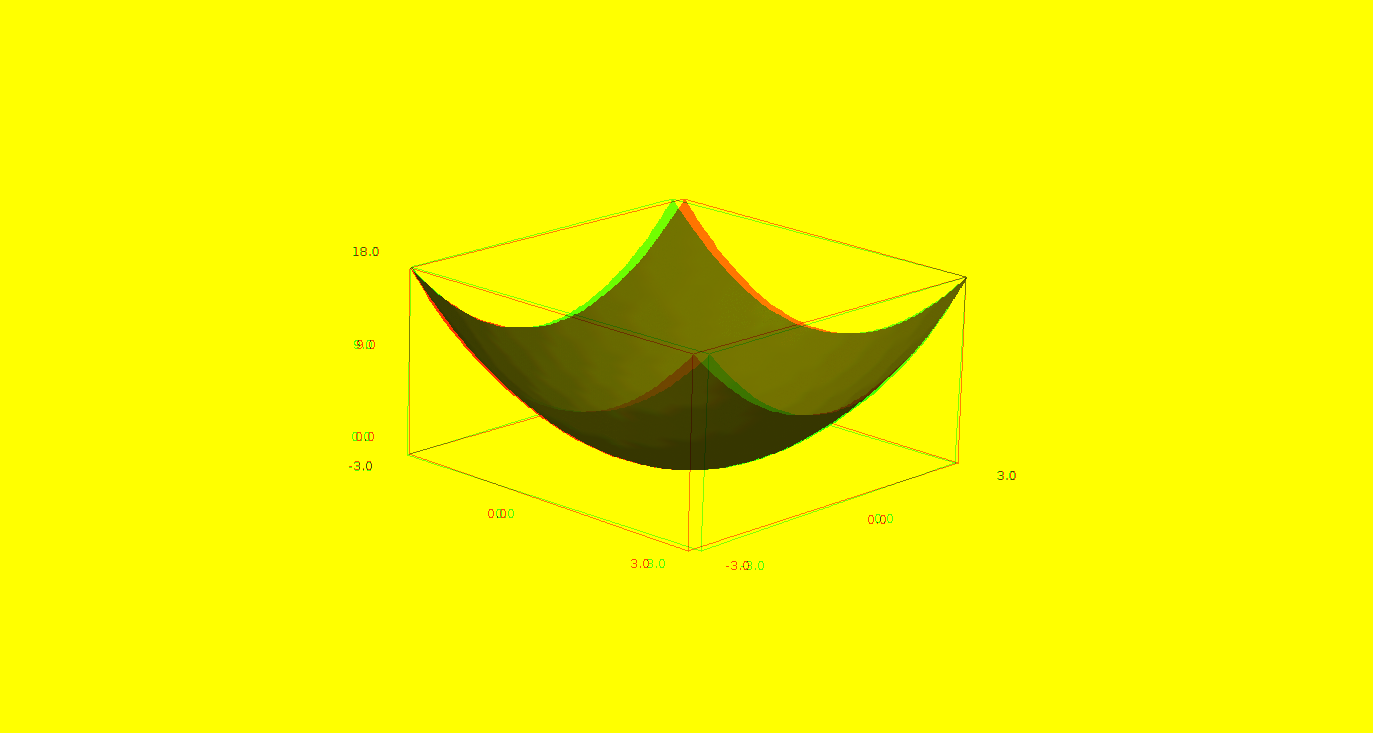
\includegraphics[width=15cm]{coupe.png}
        \else
            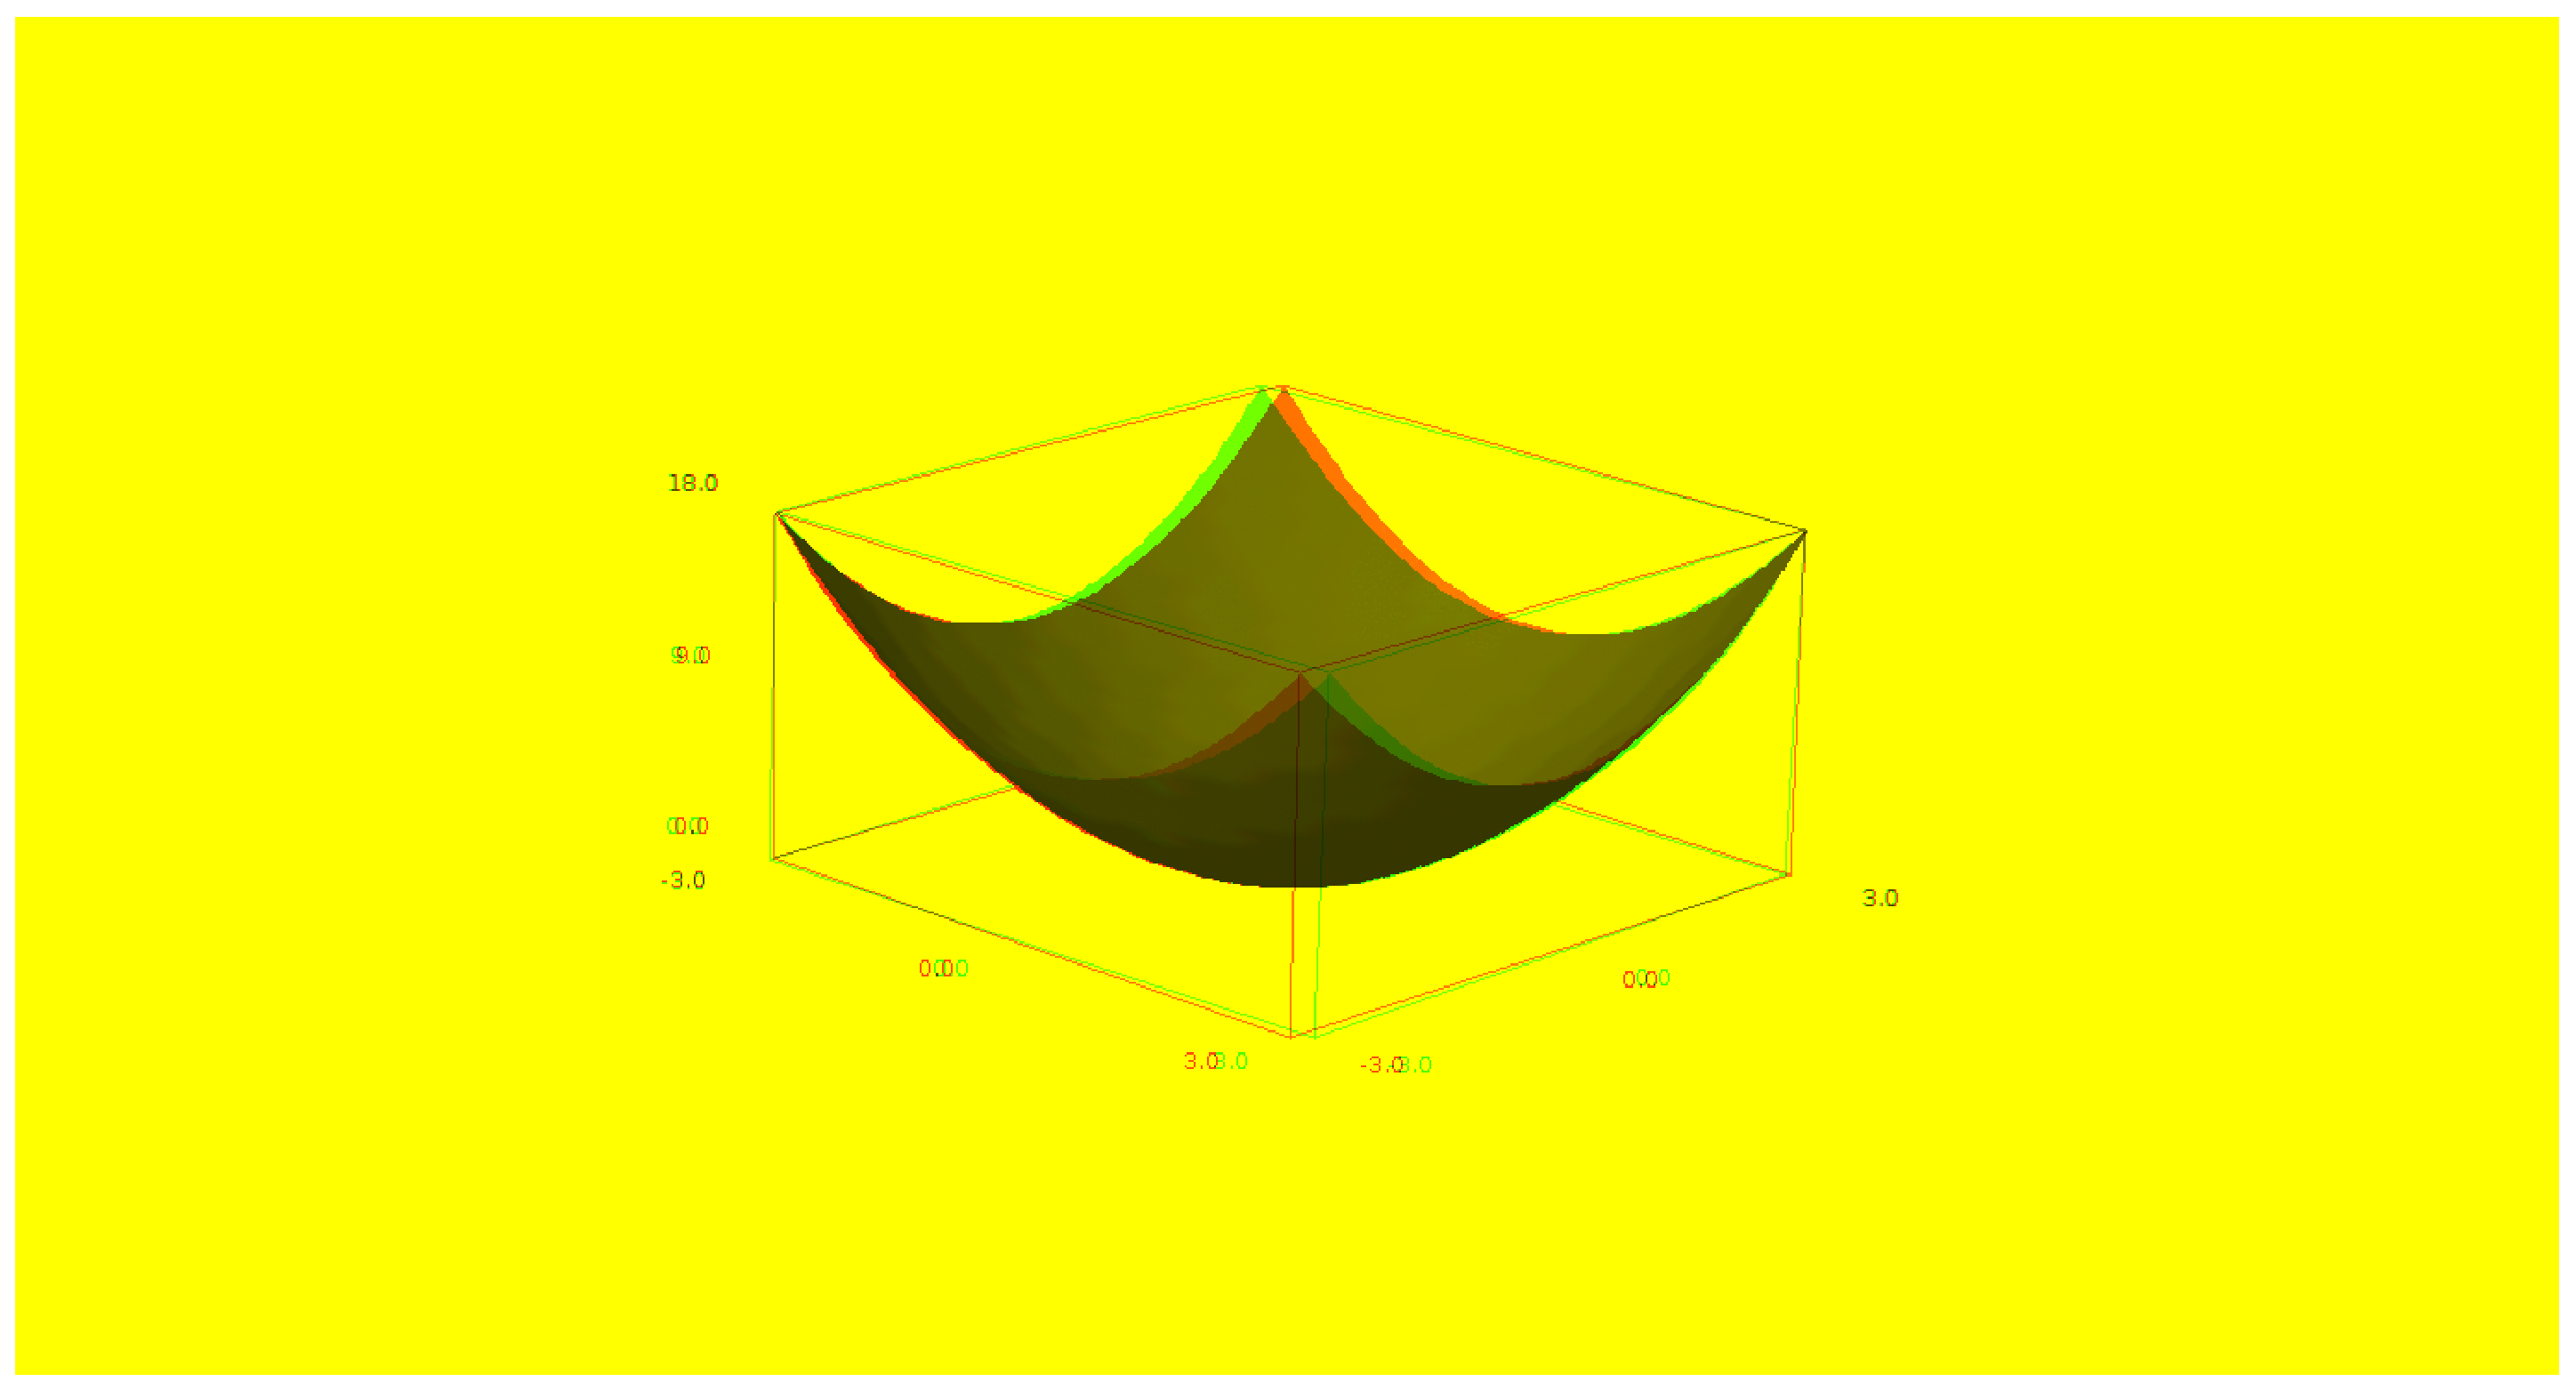
\includegraphics[width=15cm]{coupe.eps}
        \fi
    \end{center}
    À part que l'ordinateur l'a dit, est-ce qu'on peut comprendre pourquoi le graphe de la fonction $x^2+y^2$ ressemble à un bol ? En coordonnées cylindriques, le graphe s'écrit
    \begin{equation}
        z=r^2.
    \end{equation}
    Donc il se fait que plus on s'éloigne du point $(0,0)$ dans le plan $XY$, plus le graphe va monter. Et il monte à quelle vitesse ? Il monte à la vitesse $r^2$. Il s'agit donc de dessiner la fonction $z=r^2$ dans le plan et de la «faire tourner».

\end{example}

%+++++++++++++++++++++++++++++++++++++++++++++++++++++++++++++++++++++++++++++++++++++++++++++++++++++++++++++++++++++++++++
\section{Courbes de niveau}
%+++++++++++++++++++++++++++++++++++++++++++++++++++++++++++++++++++++++++++++++++++++++++++++++++++++++++++++++++++++++++++

Une technique utile pour se faire une idée de la forme d'une fonction en trois dimensions est de tracer les \defe{courbes de niveau}{courbe de niveau}. La courbe de niveau de hauteur $h$ est la courbe dans le plan donnée par l'équation
\begin{equation}
    f(x,y)=h.
\end{equation}

\begin{example}

    Dessinons par exemple les courbes de niveau de la fonction
    \begin{equation}
        f(x,y)=x+y+2.
    \end{equation}
    La courbe de niveau $h$ est donnée par l'équation $x+y+2=h$, c'est à dire
    \begin{equation}
        y(x)=-x+h-2.
    \end{equation}
    Par conséquent la courbe de niveau de hauteur $0$ est $y=-x-2$, celle de hauteur $5$ est $y=-x+3$, etc.
    
    Nous pouvons également nous aider de Sage pour ce faire :
    \begin{verbatim}
----------------------------------------------------------------------
| Sage Version 4.6.1, Release Date: 2011-01-11                       |
| Type notebook() for the GUI, and license() for information.        |
----------------------------------------------------------------------
sage: f(x,y)=x+y+2
sage: var('h')                   
h
sage: niveau(h,x)=solve(f(x,y)==h,y)[0].rhs()
sage: g1(x)=niveau(1,x)
sage: g1
x |--> -x - 1
    \end{verbatim}
    Ici la fonction \verb+g1+ est la courbe de niveau $1$. 

    Si on veut faire tracer une courbe de niveau, Sage peut le faire :
    \begin{verbatim}
        sage: implicit_plot(f(x,y)==1,(x,-3,3),(y,-4,4))
    \end{verbatim}
    Cela tracera la courbe de niveau $h=1$ dans la partie du plan $x\in\mathopen[ -3 , 3 \mathclose]$ et $y\in\mathopen[ -4,4 ,  \mathclose]$.
    
\end{example}

Il est bien entendu possible de créer automatiquement $50$ courbes de niveau et de demander de les tracer toutes sur le même graphe.
\VerbatimInput[tabsize=3]{courbeNiveau.py}

Le résultat est :

\begin{center}
    \ifpdf
        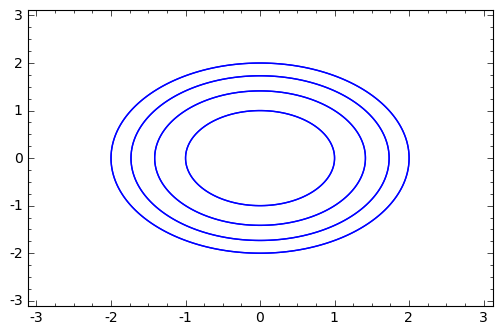
\includegraphics[width=8cm]{niveauCercles.png}
    \else
        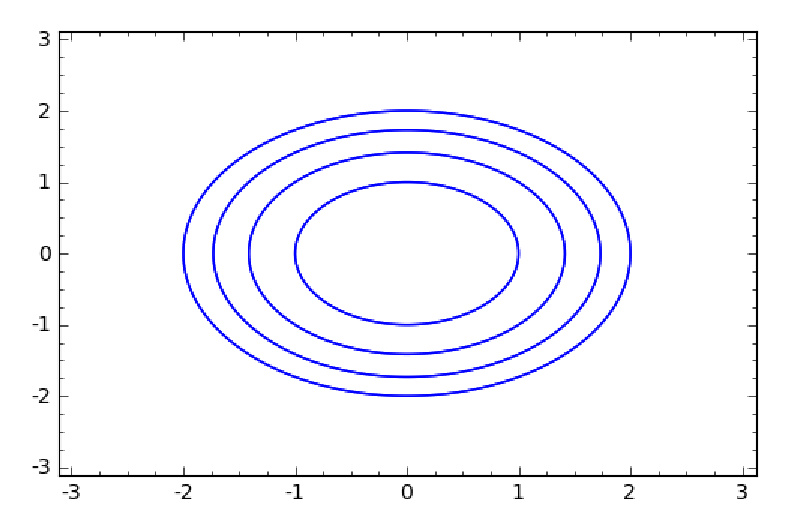
\includegraphics[width=8cm]{niveauCercles.eps}
    \fi
\end{center}
Notez que les courbes sont censées être des cercles : les axes $X$ et $Y$ n'ont pas la même échelle. Vous trouverez sur \href{http://uw.sagenb.org/home/pub/23/}{cette page} tout ce qu'il vous faudra pour créer des courbes de niveau avec Sage.

\begin{example}
    Un exemple plus riche en enseignements est celui de la fonction
    \begin{equation}
        f(x,y)=x^2-y^2.
    \end{equation}
    La courbe de niveau $h$ est donnée par l'équation $x^2-y^2=h$.

    Commençons par $h=0$. Dans ce cas nous avons $(x+y)(x-y)=0$ et par conséquent les courbes de niveau de hauteur zéro sont les deux droites $x+y=0$ et $x-y=0$.

    Voyons ensuite la courbe de niveau $h=1$. Cela est l'équation $x^2-y^2=1$, c'est à dire
    \begin{equation}
        y(x)=\pm\sqrt{x^2-1}.
    \end{equation}
    C'est une fonction qui n'est définie que pour $| x |\geq 1$. Avec $x=1$ nous avons $y=1$. Ensuite, lorsque $x$ grandit, $y$ grandit également, mais la courbe ne peut pas croiser la courbe de niveau $h=0$. Donc, suivant les notations de la figure \ref{LabelFigNiveauHyperbole}, la courbe de niveau «part» de $P$ et doit monter sans croiser les diagonales.

    \newcommand{\CaptionFigNiveauHyperbole}{La courbe de niveau $h=1$ de $x^2-y^2$. Notez qu'elle est en deux morceaux.}
    \input{Fig_NiveauHyperbole.pstricks}

    En ce qui concerne la courbe de niveau $h=-1$, elle correspond à la courbe $y=\pm\sqrt{1+x^2}$ qui est définie pour tous les $x\in\eR$. Le même raisonnement que précédemment nous amène à la figure \ref{LabelFigNiveauHyperboleDeux}.
\newcommand{\CaptionFigNiveauHyperboleDeux}{La courbe de niveau $x^2-y^2=-1$.}
\input{Fig_NiveauHyperboleDeux.pstricks}


\end{example}

Une autre façon de voir les courbe de niveau est de dire que la courbe de niveau de hauteur $h$ est la projection dans le plan $XY$ de la section du graphe de $f$ par le plan $z=h$.

On peut également définir le graphe de fonctions de trois (ou plus) variables. Le graphe de la fonction $f\colon D\subset\eR^3\to \eR$ est l'ensemble
\begin{equation}
    \big\{ \big( x,y,z,f(x,y,z) \big)\tq (x,y,z)\in D \big\}\subset \eR^4.
\end{equation}
De tels graphes ne peuvent pas être représentés sur une feuille de papier. Il est toutefois possible de définir les ensembles de niveaux :
\begin{equation}
    E_h=\big\{ (x,y,z)\in D\tq  f(x,y,z)=h\big\}.
\end{equation}
Ce sont des surfaces dans $\eR^3$ que l'on peut dessiner.

\begin{example}
    Les surfaces de niveau de la fonction $f(x,y,z)=x^2+y^2+z^2$ sont des sphères. Il n'y a pas de surfaces de niveau pour les «hauteurs» négatives.
\end{example}

\begin{example}
    Considérons la fonction $f(x,y,z)=x^2+y^2-z^2$. En coordonnées cylindrique, cette fonction s'écrit
    \begin{equation}
        f(r,\theta,z)=r^2-z^2.
    \end{equation}
    La surface de niveau $0$ est donnée par l'équation $r=| z |$. Cela fait un cercle à chaque hauteur, dont le rayon grandit linéairement avec la hauteur; le tout est donc un cône. C'est d'ailleurs le cône obtenu par rotation de la courbe de niveau $h=0$ que nous avions obtenue pour la fonction $x^2-y^2$.

    En ce qui concerne les ensembles de niveau positifs, ils sont donnés par
    \begin{equation}
        z=\pm\sqrt{x^2+y^2-h}.
    \end{equation}
    Notez qu'ils ne sont pas définis pour $r\geq h$. Cela pose un petit problème quand on veut le tracer à l'ordinateur :
    \begin{verbatim}
----------------------------------------------------------------------
| Sage Version 4.6.1, Release Date: 2011-01-11                       |
| Type notebook() for the GUI, and license() for information.        |
----------------------------------------------------------------------
sage: var('x,y')
(x, y)
sage: f(x,y)=sqrt(x**2+y**2-3)
sage: F=plot3d(f(x,y),(x,-5,5),(y,-5,5)) 
sage: G=plot3d(-f(x,y),(x,-5,5),(y,-5,5))    
sage: F+G
    \end{verbatim}
Le résultat est\footnote{Encore une fois : ça donne mieux à l'écran, et vous pouvez le faire bouger; je vous encourage à le faire !} :
    \begin{center}
        \ifpdf
            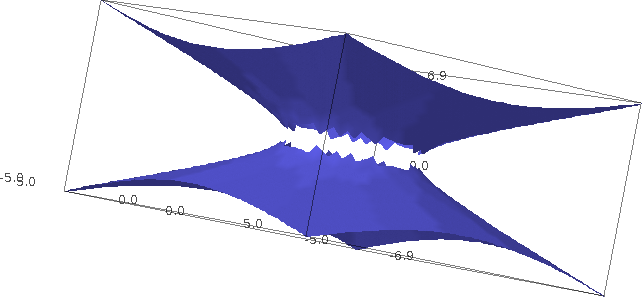
\includegraphics[width=15cm]{AdSmauvais.png}
        \else
            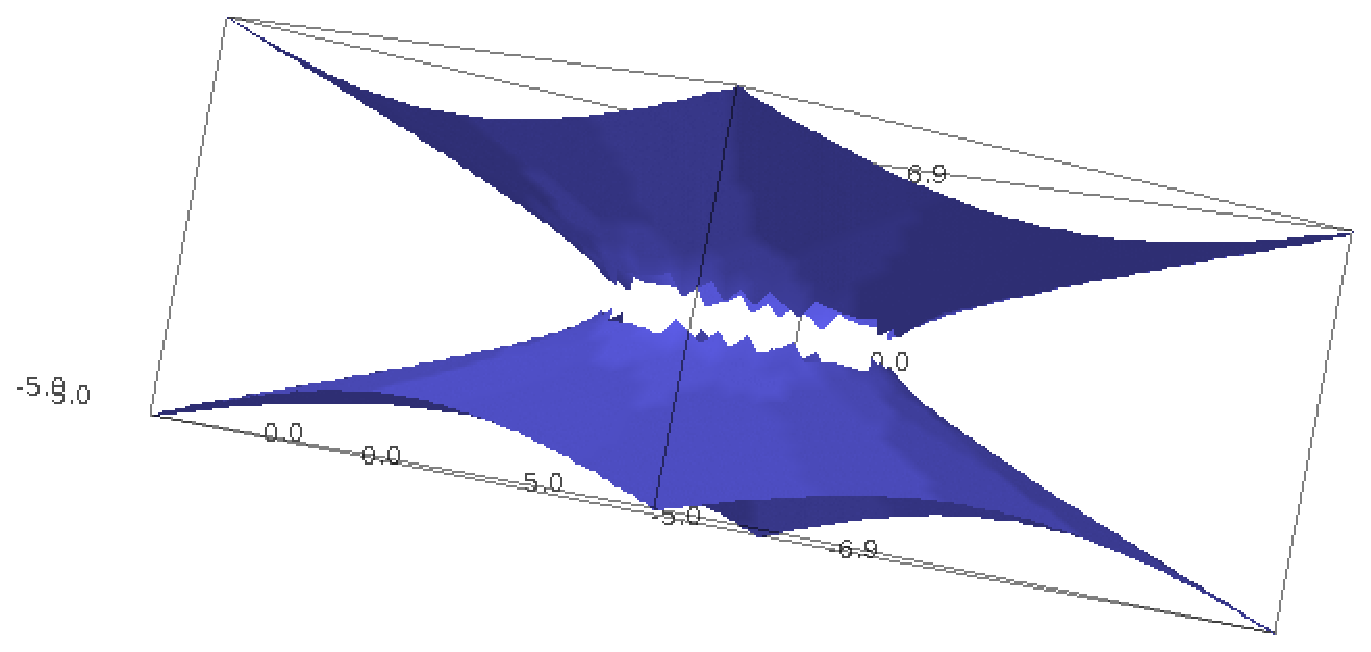
\includegraphics[width=15cm]{AdSmauvais.eps}
        \fi
    \end{center}
    On voit qu'il y a un grand trou au centre correspondant aux $z$ proches de zéro. Or d'après l'équation, il n'en est rien : en $z=0$ il y a bel et bien tout un cercle. Afin d'obtenir une meilleur image, il faut demander de tracer avec un maillage plus fin :
    \begin{verbatim}
----------------------------------------------------------------------
| Sage Version 4.6.1, Release Date: 2011-01-11                       |
| Type notebook() for the GUI, and license() for information.        |
----------------------------------------------------------------------
sage: var('x,y')
(x, y)
sage: f(x,y)=sqrt(x**2+y**2-3)
sage: F=plot3d(f(x,y),(x,-5,5),(y,-5,5),plot_points=300) 
sage: G=plot3d(-f(x,y),(x,-5,5),(y,-5,5),plot_points=300)
sage: F+G
    \end{verbatim}
    Le temps de calcul est un peu plus long, mais le résultat est meilleur :
    \begin{center}
        \ifpdf
            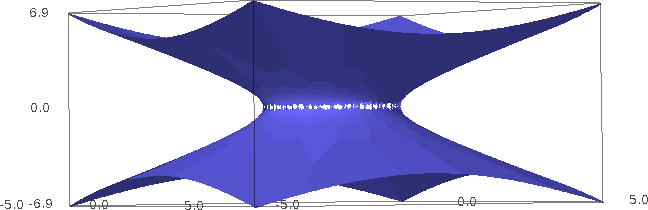
\includegraphics[width=15cm]{AdSbon.png}
        \else
            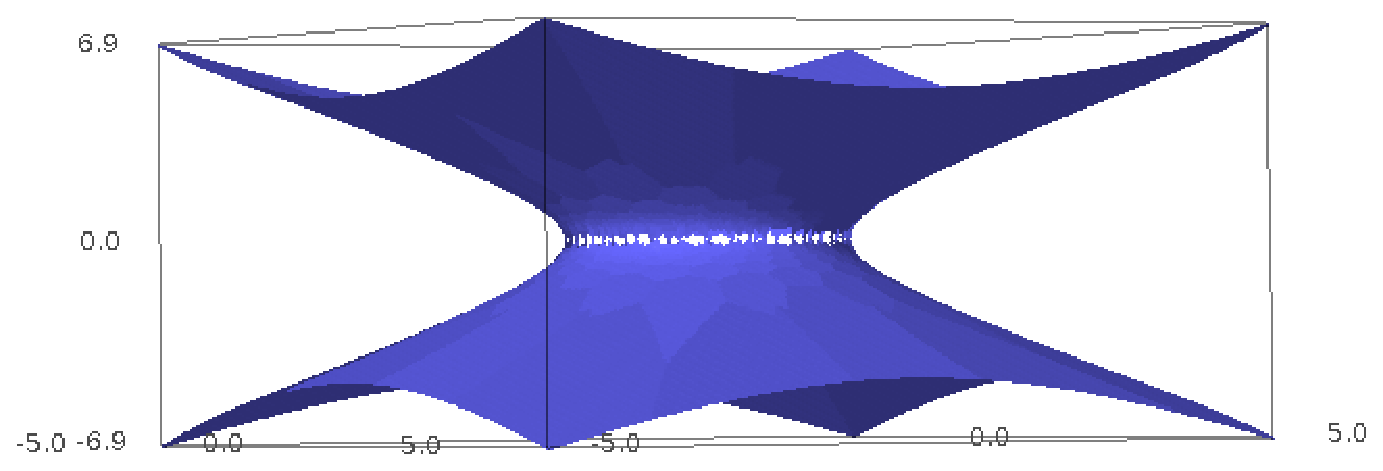
\includegraphics[width=15cm]{AdSbon.eps}
        \fi
    \end{center}
\end{example}

%+++++++++++++++++++++++++++++++++++++++++++++++++++++++++++++++++++++++++++++++++++++++++++++++++++++++++++++++++++++++++++
\section{Dérivées partielles}
%+++++++++++++++++++++++++++++++++++++++++++++++++++++++++++++++++++++++++++++++++++++++++++++++++++++++++++++++++++++++++++

Soit $f\colon \eR^2\to \eR$ une fonction de deux variables et soit $(a,b)\in\eR^2$. La façon la plus naturelle de définir une dérivée à deux variables est de considérer les \defe{dérivées partielles}{dérivée!partielle} définies par
\begin{equation}
    \begin{aligned}[]
        \frac{ \partial f }{ \partial x }(a,b)&=\lim_{x\to a} \frac{ f(x,b)-f(a,b) }{ x-a }\\
        \frac{ \partial f }{ \partial y }(a,b)&=\lim_{y\to b} \frac{ f(a,y)-f(a,b) }{y-b}.
    \end{aligned}
\end{equation}
Ces nombres représentent la façon dont le nombre $f(x,y)$ varie lorsque soit seul $x$ varie soit seul $y$ varie. Les dérivées partielles se calculent de la même façon que les dérivées normales. Pour calculer $\partial_xf$, on fait «comme si» $y$ était une constante, et pour calculer $\partial_yf$, on fait comme si $x$ était une constante.

\begin{example}
    Considérons $f(x,y)=x^2y+y^2 e^{x}$. Les dérivées partielles sont
    \begin{equation}
        \begin{aligned}[]
            \frac{ \partial f }{ \partial x }&=2xy+y^2e^x\\
            \frac{ \partial f }{ \partial y }&=x^2+2ye^x.
        \end{aligned}
    \end{equation}
\end{example}

Cet exemple était l'exemple facile où tout se passe bien.

\begin{example}
    Les choses sont moins simples lorsqu'on considère la fonction suivante :
    \begin{equation}
        f(x,y)=\begin{cases}
            \frac{ xy }{ x^2+y^2 }    &   \text{si $(x,y)\neq(0,0)$}\\
            0    &    \text{si $(x,y)=(0,0)$}.
        \end{cases}
    \end{equation}
    On voit que pour tout $x$ et tout $y$, nous avons $f(x,0)=f(0,y)=0$. Donc cette fonction est nulle sur les axes horizontaux et verticaux. Nous avons en particulier
    \begin{equation}
        \begin{aligned}[]
            \frac{ \partial f }{ \partial x }(0,0)&=0\\
            \frac{ \partial f }{ \partial y }(0,0)&=0.
        \end{aligned}
    \end{equation}
    Donc ces dérivées partielles existe.

    Il n'est par contre pas question de dire que cette fonction «va bien» autour du point $(0,0)$. En effet si nous regardons sa valeur sur la droite diagonale $y=x$, nous avons
    \begin{equation}
        f(x,x)=\frac{ x^2 }{ 2x^2 }=\frac{ 1 }{2}.
    \end{equation}
    Par conséquent si nous suivons la fonction le long de la droite $y=x$, la hauteur vaut $\frac{ 1 }{2}$ en permanence, sauf juste en $(0,0)$ où la fonction fait un grand plongeon !
    \begin{verbatim}
    sage: var('x,y')
    (x, y)
    sage: f(x,y)=(x*y)/(x**2+y**2)
    sage: plot3d(f,(x,-2,2),y(-2,2))
    \end{verbatim}

    D'ailleurs elle fait un plongeon le long de toutes les droites (sauf verticale et horizontale). En effet si nous regardons la fonction le long de la droite $y=mx$, nous avons
    \begin{equation}
        f(x,mx)=\frac{ mx^2 }{ x^2+m^2x^2 }=\frac{ m }{ 1+m^2 }.
    \end{equation}
    La fonction est donc \emph{constante} sur chacune de ces droites. Il n'est donc pas question de dire que cette fonction est «dérivable» en $(0,0)$, vu qu'elle fait des grands sauts dans presque toutes les directions.
\end{example}

Nous devons donc trouver mieux que les dérivées partielles pour étudier le comportement des fonctions un peu problématiques.

Nous nous souvenons de l'équation \eqref{EqCodeDerviffxam} qui nous dit que pour une fonction d'une variable la dérivabilité signifiait qu'il existait un nombre $\ell$ et une fonction $\alpha$ tels
\begin{equation}
    f(x)=f(a)+\ell(x-a)+(x-a)\alpha(x-a)
\end{equation}
et $\lim_{t\to 0} \alpha(t)=0$. 

En nous inspirant de cela, nous posons la définition suivante.
\begin{definition}      \label{DefDiffabel}
    Une fonction $f\colon \eR^2\to \eR$ est \defe{différentiable}{différentiable} au point $(a,b)\in\eR^2$ si il existe deux nombres $\ell_1$, $\ell_2$ ainsi qu'une fonction $\alpha$ tels que
    \begin{equation}\label{EqCondDiffabel}
        \begin{aligned}[]
            f(x,y)=f(a,b)&+\ell_1(x-a)+\ell_2(y-b)\\
                    &+\sqrt{(x-a)^2+(y-b)^2}\alpha\big( \sqrt{(x-a)^2+(y-b)^2} \big).
        \end{aligned}
    \end{equation}
\end{definition}

En utilisant la notation vectorielle, cela peut être écrite sous forme très compacte. Posons
\begin{equation}
    \begin{aligned}[]
        \ell&=\begin{pmatrix}
            \ell_1    \\ 
            \ell_2    
        \end{pmatrix},&
        X&=\begin{pmatrix}
            x    \\ 
            y    
        \end{pmatrix},&
        P&=\begin{pmatrix}
            a    \\ 
            b    
        \end{pmatrix}.
    \end{aligned}
\end{equation}
Alors la condition \eqref{EqCondDiffabel} s'écrit
\begin{equation}
    f(X)=f(P)+\ell\cdot(X-P)+\| X-P \|\alpha\big( \| X-P \| \big).
\end{equation}

\begin{proposition}
    Si $f$ est différentiable en $(a,b)$, alors les nombres $\partial_xf(a,b)$ et $\partial_yf(a,b)$ existent et valent respectivement $\ell_1$ et $\ell_2$.
\end{proposition}

\begin{proof}
    Afin de calculer la dérivée partielle dans la direction de $x$, nous posons $y=b$ dans la condition \eqref{EqCondDiffabel} :
    \begin{equation}
        f(x,b)=f(a,b)+\ell_1(x-a)+| x-a |\alpha\big( | x-a | \big),
    \end{equation}
    et donc
    \begin{equation}
        \frac{ f(x,b)-f(a,b) }{ x-a }=\ell_1\pm\alpha\big( | x-a | \big).
    \end{equation}
    Ici le $\pm$ est parce que nous avons divisé $(x-a)$ par $| x-a |$. Quel que soit ce signe, de toutes façons la limite du membre de droite lorsque $x$ tend vers $a$ est $\ell_1$ parce que $\lim_{x\to a} \alpha(| x-a |)=0$.

    Afin de prouver l'existence de la dérivée dans la direction de $y$, nous procédons de la même manière, mais en partant de $f(a,y)$.
\end{proof}

\begin{proposition}
    Si $f$ est différentiable au point $(a,b)$, alors elle y est continue, c'est à dire que
    \begin{equation}
        \lim_{(x,y)\to(a,b)}f(x,y)=f(a,b).
    \end{equation}
\end{proposition}

\begin{proof}
    Si nous considérons la différence entre $f(x,y)$ et $f(a,b)$, nous avons (en notations matricielle) :
    \begin{equation}
        | f(X)-f(P) |=| \ell\cdot(X-P)+\| X-P \|\alpha(\| X-P \|) |.
    \end{equation}
    Le membre de droite tend évidemment vers zéro lorsque $X$ tend vers $P$.
\end{proof}
    \begin{remark}
        Attention : ceci n'est pas une preuve. En effet, dans la mesure où nous n'avons même pas donné de définition de la limite, il n'est pas possible de donner une \emph{vraie} preuve de quoi que ce soit. 
    \end{remark}

Nous avons vu que l'existence des deux dérivées partielles ne permettait pas de conclure à la différentiabilité. La différentiabilité d'une fonction peut néanmoins être déduites d'une étude plus précise des dérivées partielles. Nous avons pour cela les propositions \ref{PropExistDiffUn} et \ref{PropExistDiffDeux}

\begin{proposition} \label{PropExistDiffUn}
    Soit $f$ une fonction de $x$ et $y$ et un point $(a,b)\in\eR^2$. Si les nombres $\partial_xf(a,b)$ et $\partial_yf(a,b)$ existent et si il existe une fonction $\alpha\colon \eR\to \eR$ telle que
    \begin{equation}        \label{eqCritDifffabsrt}
        \begin{aligned}[]
            f(x,y)=f(a,b)&+\frac{ \partial f }{ \partial x }(a,b)(x-a)+\frac{ \partial f }{ \partial y }(a,b)(y-b)\\
            &+\| (x,y)-(a,b) \| \alpha\Big( \| (x,y)-(a,b) \| \Big)
        \end{aligned}
    \end{equation}
    et
    \begin{equation}
        \lim_{t\to 0} \alpha(t)=0,
    \end{equation}
    alors $f$ est différentiable en $(a,b)$.
\end{proposition}
Dans cet énoncé nous avons écrit $d\big( (x,y),(a,b) \big)$ la distance entre $(x,y)$ et $(a,b)$, c'est à dire le nombre $\sqrt{(x-a)^2+(y-b)^2}$. Afin d'écrire l'équation \eqref{eqCritDifffabsrt} sous forme plus compacte, nous introduisons le vecteur
\begin{equation}
    \nabla f(a,b)=\begin{pmatrix}
        \frac{ \partial f }{ \partial x }(a,b)    \\ 
        \frac{ \partial f }{ \partial y }(a,b).    
    \end{pmatrix}
\end{equation}
L'équation \eqref{eqCritDifffabsrt} devient alors
\begin{equation}        \label{EqdiffComp}
    f(X)=f(P)+\nabla f(a,b)\cdot (X-P)+\| X-P \|\alpha\big( \| X-P \| \big).
\end{equation}
Le vecteur $\nabla f(a,b)$ est appelé le \defe{gradient}{gradient} de $f$ au point $(a,b)$.


\begin{proposition} \label{PropExistDiffDeux}
    Soit $f$ une fonction de deux variables admettant des dérivées partielles $\partial_xf(x,y)$ et $\partial_yf(x,y)$ qui sont elles-mêmes des fonctions continues de $x$ et $y$. Alors la fonction $f$ est différentiable partout.
\end{proposition}

\begin{remark}
    Tout ce qui a été dit, et tout ce qui sera dit, sur les fonctions a deux variables se généralise immédiatement aux fonctions à plus de variables. C'est dans ce but que la notation «compacte» utilisant les vecteurs est très pratique.
\end{remark}

Si nous remplaçons les accroissements $x-a$ et $y-b$ par $h$ et $k$, le critère de différentiabilité s'écrit
\begin{equation}
    \begin{aligned}[]
        f(a+h,b+k)=f(a,b)+\frac{ \partial f }{ \partial x }(a,b)h&+\frac{ \partial f }{ \partial y }(a,b)k\\
        &+\sqrt{h^2+k^2}\alpha\big( \sqrt{h^2+k^2} \big).
    \end{aligned}
\end{equation}
Le dernier terme du membre de droite tend vers zéro à une vitesse double lorsque $h$ et $k$ tendent vers zéro : d'une part parce que $\sqrt{h^2+k^2}$ tend vers zéro et d'autre part parce que $\alpha\big( \sqrt{h^2+k^2} \big)$ tend vers zéro. Nous avons donc la «bonne» approximation
\begin{equation}        \label{EqFormApproxfxyab}
    f(x,y)\simeq f(a,b)+\frac{ \partial f }{ \partial x }(a,b)(x-a)+\frac{ \partial f }{ \partial y }(a,b)(y-b).
\end{equation}
lorsque $(x,y)$ n'est pas trop loin de $(a,b)$. Cette expression est évidemment une généralisation immédiate de l'équation \eqref{EqfxdxSimeqfxfpx}. Elle exprime que l'on peut obtenir des information sur la valeur d'une fonction en $(x,y)$ si on peut calculer la fonction et ses dérivées en un point $(a,b)$ non loin de $(x,y)$.

Cette formule peut aussi être vue sous la forme suivante, plus pratique dans certains calculs :
\begin{equation}        \label{EqFormApproxfxyabDF}
    f(a+\Delta x,b+\Delta y)\simeq f(a,b)+\Delta x\frac{ \partial f }{ \partial x }(a,b)+\Delta y\frac{ \partial f }{ \partial y }(a,b).
\end{equation}

\begin{example}
    Prenons la fonction $f(x,y)=\cos(x)\sin(y)$ et calculons une approximation de
    \begin{equation}
        f\big( \frac{ \pi }{ 3 }+0.01,\frac{ \pi }{ 2 }+0.03 \big).
    \end{equation}
    D'abord les dérivées partielles sont
    \begin{equation}
        \begin{aligned}[]
            \frac{ \partial f }{ \partial x }(x,y)=-\sin(x)\sin(y)\\
            \frac{ \partial f }{ \partial y }(x,y)=\cos(x)\cos(y).
        \end{aligned}
    \end{equation}
    Nous allons utiliser l'approximation
    \begin{equation}
        f\big( \frac{ \pi }{ 3 }+0.01,\frac{ \pi }{ 2 }+0.03 \big)\simeq f\big( \frac{ \pi }{ 3 },\frac{ \pi }{2} \big)+0.01\frac{ \partial f }{ \partial x }\big( \frac{ \pi }{ 3 },\frac{ \pi }{2} \big)+0.03\frac{ \partial f }{ \partial y }\big( \frac{ \pi }{ 3 },\frac{ \pi }{2} \big).
    \end{equation}
    Nous avons
    \begin{equation}
        \begin{aligned}[]
            \frac{ \partial f }{ \partial x }\big( \frac{ \pi }{ 3 },\frac{ \pi }{2} \big)&=-\sin\frac{ \pi }{ 3 }\sin\frac{ \pi }{ 2 }=-\frac{ \sqrt{3} }{2}\\
            \frac{ \partial f }{ \partial y }\big( \frac{ \pi }{ 3 },\frac{ \pi }{2} \big)&=\cos\frac{ \pi }{ 3 }\cos\frac{ \pi }{ 2 }=0.
        \end{aligned}
    \end{equation}
    Par conséquent
    \begin{equation}
        f\big( \frac{ \pi }{ 3 }+0.01,\frac{ \pi }{ 2 }+0.03 \big)\simeq \frac{ 1 }{2}-0.01\frac{ \sqrt{3} }{2}=\frac{ 1 }{2}-\frac{ \sqrt{3} }{ 200 }. 
    \end{equation}
    
    \begin{verbatim}
sage: var('x,y')
(x, y)
sage: f(x,y)=cos(x)*sin(y)
sage: a=f(pi/3+0.01,pi/2+0.03)
sage: numerical_approx(a)
0.491093815387986
sage: b=1/2-sqrt(3)/200
sage: numerical_approx(b)
0.491339745962156
sage: numerical_approx(a-b)
-0.000245930574169814
    \end{verbatim}
    Cela fait une erreur de l'ordre du dix millième. 
    
\end{example}

\begin{remark}
    Les esprits les plus critiques diront que cette vérification pas Sage n'en est pas une parce que Sage a certainement utilisé un algorithme d'approximation qui se base sur la même idée que ce que nous venons de faire, et que par conséquent le fait qu'il obtienne le même résultat que nous est un peu tautologique. 
    
    Ils n'auront pas tord. Cependant, le code source de Sage est disponible publiquement\footnote{Voir \url{http://www.sagemath.org}}; vous pouvez aller le lire et vérifier qu'il y a effectivement une \emph{preuve} que le résultat fourni par Sage possède une bonne dizaine de décimales correctes. 
    
    Cette disponibilité publique du code source est une des nombreuses différence fondamentale entre Sage et votre calculatrice\footnote{et les autres logiciels de type fenêtre, pomme ou feuille d'érable.}. Dois-je vous rappeler qu'un des principes fondamentaux de l'éthique scientifique est que les résultats et les méthodes utilisées doivent être absolument ouverts à la vérification et à la critique de tous ?
\end{remark}

%---------------------------------------------------------------------------------------------------------------------------
\subsection{Différentielle}
%---------------------------------------------------------------------------------------------------------------------------

\begin{definition}      \label{DefDiffrdrr}
    Lorsque $f$ est différentiable au point $(a,b)$, on appelle \defe{différentielle}{différentielle} de $f$ l'application linéaire
    \begin{equation}        \label{EqDefDiffmapdf}
        \begin{aligned}
            df_{(a,b)}\colon \eR^2&\to \eR \\
            \begin{pmatrix}
                u_1    \\ 
                u_2    
            \end{pmatrix}&\mapsto \frac{ \partial f }{ \partial x }(a,b)u_1+\frac{ \partial f }{ \partial y }(a,b)u_2. 
        \end{aligned}
    \end{equation}
    En notations compacte :
    \begin{equation}        \label{EqdfUPnable}
        df_{P}(U)=\nabla f(P)\cdot U.
    \end{equation}
\end{definition}

Note : dans la suite nous allons rendre notre «notation compacte» plus agréable à lire en abandonnant les majuscules. L'équation \eqref{EqdfUPnable} s'écrira donc
\begin{equation}        \label{Eqdfpunfpdu}
    df_p(u)=\nabla f(p)\cdot u.
\end{equation}


%+++++++++++++++++++++++++++++++++++++++++++++++++++++++++++++++++++++++++++++++++++++++++++++++++++++++++++++++++++++++++++
\section{Plan tangent au graphe d'une fonction}
%+++++++++++++++++++++++++++++++++++++++++++++++++++++++++++++++++++++++++++++++++++++++++++++++++++++++++++++++++++++++++++

Nous avons vu que, de la même façon qu'en deux dimensions nous avions l'approximation \eqref{Eqfxsimesfa} d'une fonction par sa tangente, en trois dimensions nous avons l'approximation suivante d'une fonction de deux variables :
\begin{equation}
    f(x,y)\simeq f(a,b)+\frac{ \partial f }{ \partial x }(a,b)(x-a)+\frac{ \partial f }{ \partial y }(a,b)(y-b)
\end{equation}
lorsque $(x,y)$ n'est pas trop loin de $(a,b)$. Cela signifie que le graphe de $f$ ressemble au graphe de la fonction $T_{(a,b)}$ donnée par
\begin{equation}
    T_{(a,b)}(x,y)=f(a,b)+\frac{ \partial f }{ \partial x }(a,b)(x-a)+\frac{ \partial f }{ \partial y }(a,b)(x-a).
\end{equation}
En notations compactes :
\begin{equation}
    T_p(x)=f(p)+\nabla f(p)\cdot (x-p).
\end{equation}
Le graphe de la fonction $T_p$ sera le \defe{plan tangent}{plan!tangent} au graphe de $f$ au point $p$. L'équation du plan tangent sera donc
\begin{equation}
    z-f(p)=\nabla f(p)\cdot (x-p).
\end{equation}

\begin{remark}
    Lorsque nous utilisons la notation vectorielle, la lettre «$x$» désigne le vecteur $(x,y)$. Il faut être attentif. Dans un cas $x$ est un vecteur dans l'autre c'est une composante d'un vecteur.
\end{remark}




%+++++++++++++++++++++++++++++++++++++++++++++++++++++++++++++++++++++++++++++++++++++++++++++++++++++++++++++++++++++++++++
\section{Dérivée directionnelle}
%+++++++++++++++++++++++++++++++++++++++++++++++++++++++++++++++++++++++++++++++++++++++++++++++++++++++++++++++++++++++++++

Nous sommes capables de dériver une fonction de deux variables $f(x,y)$ par rapport à $x$ et par rapport à $y$. C'est à dire que nous sommes capables de donner la variation de la fonction lorsqu'on bouge le long des axes horizontal et vertical. Il est évidemment souhaitable de parler de la variation de la fonction lorsqu'on se déplace le long d'autre droites.

Soit donc $u=\begin{pmatrix}
    u_1    \\ 
    u_2    
\end{pmatrix}$ un vecteur unitaire (c'est à dire $u_1^2+u_2^2=1$), et considérons la fonction de une variable
\begin{equation}
    \begin{aligned}
        \varphi\colon \eR&\to \eR \\
        t&\mapsto f(a+tu_1,b+tu_2). 
    \end{aligned}
\end{equation}
La fonction $\varphi$ n'est rien d'autre que la fonction $f$ vue le long de la droite de direction donnée par le vecteur $u$. Nous pouvons aussi l'écrire $\varphi(t)=f(p+tu)$.

\begin{proposition}
    Si $f$ est différentiable en $(a,b)$ alors la fonction $\varphi$ est dérivable en $0$ et on a
    \begin{equation}
        \varphi'(0)=\nabla f(p)\cdot u
    \end{equation}
    où nous avons noté $p=(a,b)$.
\end{proposition}

\begin{proof}
    Récrivons la formule \eqref{EqdiffComp} sous la forme
    \begin{equation}
        f(x)=f(p)+\nabla f(p)\cdot (x-p)+\| x-p \|\alpha(\| x-p \|).
    \end{equation}
    Cela étant vrai pour tout $x$, nous l'écrivons en particulier pour $x=p+tu$ où $t$ est un réel et $u$ est le vecteur unitaire choisi. Nous avons donc
    \begin{equation}
        f(p+tu)=f(p)+t\nabla f(p)\cdot u+\| tu \|\alpha(\| tu \|).
    \end{equation}
    En utilisant le fait que $u$ est unitaire, $\| tu \|=| t |\| u \|=| t |$. La dérivée de $\varphi$ en $0$ est alors donnée par
    \begin{equation}
        \lim_{t\to 0} \frac{ f(p+tu)-f(p) }{ t }=\lim_{t\to 0} \nabla f(p)\cdot u+\alpha(| t |).    
    \end{equation}
    Lorsque nous prenons la limite, le membre de gauche devient $\varphi'(0)$ tandis que dans le membre de droite, le second terme disparaît. Nous avons finalement
    \begin{equation}
        \varphi'(0)=\nabla f(p)\cdot u
    \end{equation}
\end{proof}

\begin{definition}
    Le nombre
    \begin{equation}
        \lim_{t\to 0} \frac{ f\big( a+tu_1,b+tu_2 \big)-f(a,b) }{ t }
    \end{equation}
    est la \defe{dérivée directionnelle}{dérivée!directionnelle} de $f$ dans la direction de $u$ au point $(a,b)$. Il sera noté
    \begin{equation}
        \frac{ \partial f }{ \partial u }(a,b),
    \end{equation}
    ou plus simplement $\partial_uf(a,b)$.
\end{definition}

Lorsque $f$ est différentiable, la dérivée directionnelle est donnée par
\begin{equation}        \label{EqDerDirnablau}
    \frac{ \partial f }{ \partial u }(p)=\nabla f(p)\cdot u.
\end{equation}

En combinant avec l'équation \eqref{Eqdfpunfpdu}, nous avons la suite d'égalités
\begin{equation}        \label{Eqsuitedfnfdsdfu}
    df_p(u)=\nabla f(p)\cdot u=\frac{ \partial f }{ \partial x }(p)u_1+\frac{ \partial f }{ \partial y }(p)u_2+\frac{ \partial f }{ \partial z }(p)u_3=\frac{ \partial f }{ \partial u }(p).
\end{equation}
La dernière équation est seulement vraie si $\| u \|=1$.

%---------------------------------------------------------------------------------------------------------------------------
\subsection{Gradient : direction de plus grande pente}
%---------------------------------------------------------------------------------------------------------------------------

Étant donné que $u$ est de norme $1$, l'inégalité de Cauchy-Schwartz donne
\begin{equation}
    \big| \nabla f(a,b)\cdot \begin{pmatrix}
        u_1    \\ 
        u_2    
    \end{pmatrix}\big|\leq \| \nabla f(a,b) \|.
\end{equation}
Donc
\begin{equation}
    -\| \nabla f(p) \|\leq \nabla f(p)\cdot u\leq\| \nabla f(p) \|.
\end{equation}
La norme de la dérivée directionnelle (qui est la valeur absolue du nombre au centre) est donc «coincée» entre $-\| \nabla f(p) \|$ et $\| \nabla f(p) \|$. Prenons par exemple
\begin{equation}
    u=\frac{ \nabla f(p) }{ \| \nabla f(p) \| }.
\end{equation}
Dans ce cas, nous avons exactement
\begin{equation}
    \nabla f(p)\cdot u=\| \nabla f(p) \|,
\end{equation}
qui est la valeur maximale que la dérivée directionnelle peut prendre.

La direction du gradient est donc la direction suivant laquelle la dérivée directionnelle est la plus grande. Pour la même raison, la dérivée directionnelle est la plus petite dans le sens opposé au gradient.

En termes bien clairs : lorsqu'on veut aller le plus vite possible au ski, on prend la direction du gradient de la piste de ski. C'est dans cette direction que ça descend le plus vite. Dans quelle direction vont les débutants ? Ils vont perpendiculairement à la pente (ce qui ennuie tout le monde, mais c'est un autre problème). Les débutants vont donc dans la direction perpendiculaire au gradient. Prenons donc $u\perp \nabla f(p)$ et calculons la dérivée directionnelle de $f$ dans la direction $u$ en utilisant la formule \ref{EqDerDirnablau} :
\begin{equation}
    \frac{ \partial f }{ \partial u }(p)=\nabla f(p)\cdot u=0
\end{equation}
parce que nous avons choisi $u\perp \nabla f(p)$. Nous voyons donc que les débutants en ski ont eu la bonne intuition que la direction dans laquelle la piste ne descend pas, c'est la direction perpendiculaire au gradient.

C'est aussi pour cela que l'on a tendance à faire du zig-zag à vélo lorsqu'on monte une pente très forte et qu'on est fatigué. C'est toujours pour cela que les routes de montagne font de longs lacets. La montée est moins rude en suivant une direction proche d'être perpendiculaire au gradient !

\begin{theorem}
    Le gradient des fonction suit à peu près les mêmes règles que les dérivées. Soient $f$ et $g$ deux fonctions différentiables. Nous avons entre autres
    \begin{enumerate}
        \item
            $\nabla(f+g)=\nabla f+\nabla g$;
        \item
            $\nabla(fg)(a,b)=g(a,b)\nabla f(a,b)+f(a,b)\nabla g(a,b)$;
        \item
            Dès que $g(a,b)\neq 0$, nous avons
            \begin{equation}
                \nabla\frac{ f }{ g }=\frac{ g(a,b)\nabla f(a,b)-f(a,b)\nabla g(a,b) }{ g(a,b)^2 }.
            \end{equation}
    \end{enumerate}
\end{theorem}

% This is part of Mes notes de mathématique
% Copyright (c) 2011-2012
%   Laurent Claessens
% See the file fdl-1.3.txt for copying conditions.

Les champs de vecteurs et tout ce qui s'y rapportent jouent un rôle crucial en électromagnétisme. Voir par exemple \cite{Schomblond_em}.

%+++++++++++++++++++++++++++++++++++++++++++++++++++++++++++++++++++++++++++++++++++++++++++++++++++++++++++++++++++++++++++
\section{Les fonctions à valeurs vectorielles}
%+++++++++++++++++++++++++++++++++++++++++++++++++++++++++++++++++++++++++++++++++++++++++++++++++++++++++++++++++++++++++++

Jusqu'à présent nous avons vu des fonctions de plusieurs variables qui prenaient leurs valeurs dans $\eR$. Nous allons maintenant voir ce qu'il se passe lorsque les fonctions prennent leurs valeurs dans $\eR^3$.

Une fonction d'une variable est dite \defe{à valeurs vectorielles}{fonction!valeurs vectorielles} lorsque
\begin{equation}
    \begin{aligned}
        f\colon I\subset \eR&\to \eR^3 \\
        f(x)&=\begin{pmatrix}
            f_1(x)    \\ 
            f_2(x)    \\ 
            f_3(x)    
        \end{pmatrix}.
    \end{aligned}
\end{equation}
Les fonctions $f_i\colon \eR\to \eR$ sont les \defe{composantes}{composante} de $f$. Ce que nous avons raconté à propos des dérivées passe facilement :
\begin{equation}
    \frac{ f(a+\epsilon)-f(a) }{ \epsilon }=
    \begin{pmatrix}
        \frac{ f_1(a+\epsilon)-f_1(a) }{ \epsilon }    \\ 
        \frac{ f_2(a+\epsilon)-f_2(a) }{ \epsilon }    \\ 
        \frac{ f_3(a+\epsilon)-f_3(a) }{ \epsilon }    
    \end{pmatrix}.
\end{equation}
En particulier dès que les fonctions $f_i$ sont dérivables, nous avons
\begin{equation}
    f'(a)=\begin{pmatrix}
        f_1'(a)    \\ 
        f_2'(a)    \\ 
        f_3'(a)    
    \end{pmatrix}
\end{equation}
comme dérivée de la fonction. Cette dérivée est un vecteur.

\begin{example}
    Si
    \begin{equation}
        f\colon x\in\eR\mapsto \begin{pmatrix}
            x^2 e^{x}    \\ 
            \cos(x^2)    \\ 
            x^3+x    
        \end{pmatrix},
    \end{equation}
    alors
    \begin{equation}
        f'(x)=\begin{pmatrix}
            2xe^x+x^2e^x    \\ 
            -2x\sin(x^2)    \\ 
            3x^2+1    
        \end{pmatrix}.
    \end{equation}
\end{example}

%+++++++++++++++++++++++++++++++++++++++++++++++++++++++++++++++++++++++++++++++++++++++++++++++++++++++++++++++++++++++++++
\section{Fonctions vectorielles de plusieurs variables}
%+++++++++++++++++++++++++++++++++++++++++++++++++++++++++++++++++++++++++++++++++++++++++++++++++++++++++++++++++++++++++++

Ce sont les fonctions de la forme
\begin{equation}
    \begin{aligned}
        f\colon \eR^3&\to \eR^3 \\
        \begin{pmatrix}
            x    \\ 
            y    \\ 
            z    
        \end{pmatrix}&\mapsto \begin{pmatrix}
            f_1(x,y,z)\\
            f_2(x,y,z)\\
            f_3(x,y,z)
        \end{pmatrix}.
    \end{aligned}
\end{equation}

En ce qui concerne les dérivées, tout se passe comme avant. Si les dérivées partielles des composantes $f_i$ existent au point $a\in\eR^3$, alors
\begin{equation}
    \begin{aligned}[]
        \frac{ \partial f }{ \partial x }(a)&=\begin{pmatrix}
            \partial_xf_1(a)    \\ 
            \partial_xf_2(a)    \\ 
            \partial_xf_3(a)    \\ 
        \end{pmatrix},&
        \frac{ \partial f }{ \partial y }(a)&=\begin{pmatrix}
            \partial_yf_1(a)    \\ 
            \partial_yf_2(a)    \\ 
            \partial_yf_3(a)    \\ 
        \end{pmatrix},&
        \frac{ \partial f }{ \partial z }(a)&=\begin{pmatrix}
            \partial_zf_1(a)    \\ 
            \partial_zf_2(a)    \\ 
            \partial_zf_3(a)    \\ 
        \end{pmatrix}.
    \end{aligned}
\end{equation}

%+++++++++++++++++++++++++++++++++++++++++++++++++++++++++++++++++++++++++++++++++++++++++++++++++++++++++++++++++++++++++++
\section{Champs de vecteurs}
%+++++++++++++++++++++++++++++++++++++++++++++++++++++++++++++++++++++++++++++++++++++++++++++++++++++++++++++++++++++++++++

Un champ de vecteur est une fonction $f\colon \eR^3\to \eR^3$. Géométriquement, il s'agit simplement de mettre un vecteur en chaque point de l'espace. Cela arrive très souvent en physique.

\begin{example}
    Si un fluide (eau, gaz) coule dans un tube, en tout point le point a une vitesse, qui sera un vecteur généralement dirigé le long du tube.
\end{example}

\begin{example}
    La force d'attraction de la Terre sur une masse $m$ située au point $r=(x,y,z)$ est donnée par
    \begin{equation}
        F(r)=-G\frac{ Mmr }{ \| r \|^3 }.
    \end{equation}
    Dans cette expression, tant $r$ que $F(r)$ sont des vecteurs. Nous l'avons représenté sur la figure \ref{LabelFigChampGraviation}.
    \newcommand{\CaptionFigChampGraviation}{Le champ de gravitation de la Terre.}
    \input{Fig_ChampGraviation.pstricks}

    L'application
    \begin{equation}
        \begin{aligned}
            F\colon \eR^3&\to \eR^3 \\
            r&\mapsto F(r) 
        \end{aligned}
    \end{equation}
    est le champ gravitationnel de la Terre.

\end{example}

%---------------------------------------------------------------------------------------------------------------------------
\subsection{Matrice jacobienne}
%---------------------------------------------------------------------------------------------------------------------------

La \defe{matrice jacobienne}{jacobien} de la fonction $f\colon \eR^3\to \eR^3$ au point $a\in\eR^3$ est la matrice dont les colonnes sont les vecteurs $\frac{ \partial f }{ \partial x }(a)$, $\frac{ \partial f }{ \partial y }(a)$ et $\frac{ \partial f }{ \partial z }(a)$, c'est à dire
\begin{equation}
    J_f(a)=\begin{pmatrix}
        \frac{ \partial f_1 }{ \partial x }(a)   &   \frac{ \partial f_1 }{ \partial y }(a)    &   \frac{ \partial f_1 }{ \partial z }(a)    \\
        \frac{ \partial f_2 }{ \partial x }(a)   &   \frac{ \partial f_2 }{ \partial y }(a)    &   \frac{ \partial f_2 }{ \partial z }(a)    \\
        \frac{ \partial f_3 }{ \partial x }(a)   &   \frac{ \partial f_3 }{ \partial y }(a)    &   \frac{ \partial f_3 }{ \partial z }(a)    
    \end{pmatrix}.
\end{equation}

\begin{example}
    Si 
    \begin{equation}
        f(x,y,z)=\begin{pmatrix}
            xy e^{z}    \\ 
            x^2+\cos(yz)    \\ 
            xyz    
        \end{pmatrix},
    \end{equation}
    alors
    \begin{equation}
        J_f(x,y,z)=\begin{pmatrix}
            ye^z    &   xe^z    &   xye^z    \\
            2x    &   -z\sin(yz)    &   -y\sin(yz)    \\
            yz    &   xz    &   xy
        \end{pmatrix}.
    \end{equation}
\end{example}

%+++++++++++++++++++++++++++++++++++++++++++++++++++++++++++++++++++++++++++++++++++++++++++++++++++++++++++++++++++++++++++
\section{Courbes paramétrés}
%+++++++++++++++++++++++++++++++++++++++++++++++++++++++++++++++++++++++++++++++++++++++++++++++++++++++++++++++++++++++++++

%---------------------------------------------------------------------------------------------------------------------------
\subsection{Définitions et exemples}
%---------------------------------------------------------------------------------------------------------------------------

\begin{definition}
    Un \defe{chemin}{chemin} dans $\eR$ est une application continue
    \begin{equation}
        \begin{aligned}
            \sigma\colon [a,b]&\to \eR^3 \\
            t&\mapsto \sigma(t). 
        \end{aligned}
    \end{equation}
\end{definition}

La fonction $\sigma'(t)$ est la \defe{vitesse}{vitesse d'un chemin} du chemin $\sigma$. Si la fonction $t\mapsto\sigma(t)$ est dérivable, on dit que $\sigma''(t)$ est l'\defe{accélération}{accélération d'un chemin}. Les points $\sigma(a)$ et $\sigma(b)$ sont les extrémités du chemin. L'ensemble
\begin{equation}
    \{ \sigma(t)\tq t\in\mathopen[ a , b \mathclose] \}
\end{equation}
est la \defe{courbe}{courbe} $\sigma$.

\begin{example}
    Soit $v\in\eR^3$ et $x_0\in\eR^3$. Le chemin
    \begin{equation}
        \sigma(t)=x_0+tv
    \end{equation}
    est une droite. Sa vitesse est $\sigma'(t)=v$.    
\end{example}

\begin{example}
    La courbe
    \begin{equation}
        \sigma(t)=\begin{pmatrix}
            \cos(t)    \\ 
            \sin(t)    
        \end{pmatrix}\in\eR^2
    \end{equation}
    avec $t\in\mathopen[ 0 , 2\pi [$ est le cercle unité parcouru une fois dans le sens trigonométrique.

    Notez que si on prend $t\in\mathopen[ 0 , 4\pi [$, nous avons un \emph{autre} chemin; c'est le même cercle unité, mais parcouru \emph{deux} fois. Même si le «dessin» (le graphe) des deux est le même, le chemin n'est pas le même.

    Le chemin
    \begin{equation}
        \gamma(t)=\begin{pmatrix}
            \cos(2\pi-t)    \\ 
            \sin(2\pi-t)    
        \end{pmatrix}
    \end{equation}
    est le cercle unité parcouru une fois dans le sens inverse. Encore une fois le «dessin» est le même, mais le chemin n'est pas le même.
\end{example}

\begin{example}
    Le chemin
    \begin{equation}
        \sigma(t)=\begin{pmatrix}
            t    \\ 
            t^2    
        \end{pmatrix}
    \end{equation}
    est un chemin dont l'image est la parabole d'équation $y=x^2$.
\end{example}

L'importance de la dérivée du chemin réside en le fait qu'elle donne la tangente. En effet le vecteur $\sigma'(t)$ est tangent au graphe de $\sigma$ au point $\sigma(t)$.
\begin{example}
    Pour le cercle,
    \begin{equation}
        \sigma(t)=\begin{pmatrix}
            \cos(t)    \\ 
            \sin(t)    
        \end{pmatrix},
    \end{equation}
    la dérivée est donnée par
    \begin{equation}
        \sigma'(t)=\begin{pmatrix}
            -\sin(t)    \\ 
            \cos(t).    
        \end{pmatrix}
    \end{equation}
    Le produit scalaire $\sigma(t)\cdot \sigma'(t)$ est nul. Le vecteur $\sigma'(t)$ est donc bien tangent (voir exercice \ref{exoDerive-0003}).
\end{example}

\begin{example}
    Le courbe donnée par le chemin
    \begin{equation}
        \sigma(t)=\begin{pmatrix}
            \cos(t)    \\ 
            \sin(t)    \\ 
            t    
        \end{pmatrix}
    \end{equation}
    est une hélice. Sa vitesse est
    \begin{equation}
        \sigma'(t)=\begin{pmatrix}
            -\sin(t)    \\ 
            \cos(t)    \\ 
            1    
        \end{pmatrix}.
    \end{equation}
    Notez que pour tout $t\in\eR$, nous avons $\| \sigma'(t) \|=\sqrt{2}$.
\end{example}

\begin{remark}
    Lorsqu'on parle d'une courbe dans l'espace, l'intervalle sur lequel on considère la variation du paramètre est une donné fondamentale. Elle fait partie intégrante de la définition de la courbe.
\end{remark}

%---------------------------------------------------------------------------------------------------------------------------
\subsection{Longueur d'une courbe paramétrée}
%---------------------------------------------------------------------------------------------------------------------------

Nous pouvons voir un chemin $\sigma$ comme étant la trajectoire d'une particule en fonction du temps. Sa vitesse à l'instant $t$ est le vecteur $\sigma'(t)$, tandis que sa vitesse \emph{scalaire} est le nombre $\| \sigma'(t) \|$. Une question naturelle est de savoir quelle est la longueur de la trajectoire parcourue entre $t=a$ et $t=b$.

Si nous prenons un petit intervalle de temps $dt$, nous pouvons supposer que le mobile avance à la vitesse constante $\| \sigma'(t) \|$. Cela ferait un trajet parcouru de longueur $\| \sigma'(t) \|dt$. Nous prenons donc la définition suivante pour la longueur.

\begin{definition}
    Soit $\sigma\colon \mathopen[ a , b \mathclose]\to \eR^3$ un chemin. La \defe{longueur}{longueur!d'un chemin} du chemin $\sigma$ est le nombre
    \begin{equation}        \label{EqDefLongueurChemin}
        l(\sigma)=\int_a^b\| \sigma'(t) \|dt.
    \end{equation}
    Plus explicitement, si $\sigma(t)=\big( x(t),y(t),z(t) \big)$, alors nous avons la formule
    \begin{equation}
        l(\sigma)=\int_a^b\sqrt{x'(t)^2+y'(t)^2+z'(t)^2}dt.
    \end{equation}
\end{definition}

\begin{example}
    Considérons l'arc de cercle de rayon $R$ interceptée par l'angle $\theta$ présenté sur la figure \ref{LabelFigAMDUooZZUOqa}. % From file AMDUooZZUOqa                                                         
\newcommand{\CaptionFigAMDUooZZUOqa}{Quelle est la longueur de la partie bleue de ce cercle de rayon $R$ ?}                                            
\input{Fig_AMDUooZZUOqa.pstricks} 
    
    Par définition, cette longueur sera
    \begin{equation}
        \int_{\theta_0}^{\theta_1}\sqrt{R^2\sin^2(t)+R^2\cos^2(t)}dt=R(\theta_1-\theta_0).
    \end{equation}
    Le radian comme unité de mesure d'angle est donc l'unité parfaite : elle est la longueur d'arc interceptée (si le rayon est $R=1$).
\end{example}

\begin{example}
    La longueur de l'hélice
    \begin{equation}
        \sigma(t)=\begin{pmatrix}
            \cos(2t)    \\ 
            \sin(2t)    \\ 
            \sqrt{5}t    
        \end{pmatrix}
    \end{equation}
    pour $t\in\mathopen[ 0 , 2\pi \mathclose]$ est donnée par
    \begin{equation}
        l(\sigma)=\int_0^{4\pi}\sqrt{4\sin^2(2t)+4\cos^2(2t)+5}dt=\int_0^{4\pi}\sqrt{9}=12\pi.
    \end{equation}
\end{example}

\begin{definition}
    Soit $\sigma_1\colon \mathopen[ a , b \mathclose]\to \eR^3$, un chemin et $\sigma_2\colon \mathopen[ c , d \mathclose]\to \eR^3$, un autre chemin. On dit que ces chemins sont \defe{équivalents}{equivalence@équivalence!chemin} si il existe une fonction $\varphi\colon \mathopen[ a , b \mathclose]\to \mathopen[ c , d \mathclose]$ strictement croissante telle que $\sigma_1(t)=\sigma_2\big( \varphi(t) \big)$.
\end{definition}

Deux chemins équivalents parcourent la même courbe dans le même sens. Ils ne le parcourent toutefois pas à la même vitesse. On dit que les chemins sont \defe{opposée}{opposés!chemins} si la fonction $\varphi$ de la définition est strictement décroissante. Dans ce cas, ils ont la même image, mais parcourue dans le sens opposés. Nous disons que deux chemins équivalents sont un \defe{changement de paramétrisation}{paramétrisation} pour la même courbe.

 Dans le cas d'une paramétrisation équivalente, nous avons $\varphi(a)=c$ et $\varphi(b)=d$. Les points de départ et d'arrivée des deux paramètres coïncident. Dans le cas d'un paramètre qui va dans le sens opposé par contre nous avons automatiquement $\varphi(a)=d$ et $\varphi(b)=c$.

\begin{proposition}
    La longueur d'une courbe ne dépend pas du paramètre (équivalent ou opposé) choisi.
\end{proposition}

\begin{proof}
    Soient $\sigma_1\colon \mathopen[ a , b \mathclose]\to \eR^3$ et $\sigma_2\colon \mathopen[ c , d \mathclose]\to \eR^3$ tels que
    \begin{equation}     \label{EqChmsigmaundeuxvp}
        \sigma_1(t)=\sigma_2\big( \varphi(t) \big)
    \end{equation}
    où $\varphi\colon \mathopen[ a , b \mathclose]\to \mathopen[ a , d \mathclose]$ est une bijection strictement monotone. Par définition on a
    \begin{equation}
        l(\sigma_1)=\int_a^b\| \sigma_1'(t) \|dt.
    \end{equation}
    Nous pouvons exprimer la dérivée de $\sigma_1$ en termes de celle de $\sigma_2$ en dérivant la relation \eqref{EqChmsigmaundeuxvp} :
    \begin{equation}
        \sigma_1'(t)=\varphi'(t)\sigma_2'\big( \varphi(t) \big).
    \end{equation}
    En ce qui concerne la norme,
    \begin{equation}
        \| \sigma_1'(t) \|=| \varphi'(t) |\| \sigma_2'(t) \|.
    \end{equation}
    Notez dans cette relation que $\varphi'(t)$ est un nombre (et non un vecteur). Étant donné que nous avons supposé que $\varphi$ était monotone, soit elle est monotone croissante et $\| \varphi'(t) \|=\varphi'(t)$ pour tout $t$, soit elle est monotone décroissante et $\| \varphi'(t) \|='\varphi(t)$ pour tout $t$.

    Considérons d'abord le premier cas, c'est à dire $\| \varphi'(t) \|=\varphi'(t)$. Nous posons $s=\varphi(t)$, $ds=\varphi'(t)dt$. En remplaçant cela dans la formule de la longueur est
    \begin{equation}
        \begin{aligned}[]
            l(\sigma_1)&=\int_a^b\varphi'(t)\| \sigma_2\big( \varphi(t) \big) \|dt\\
            &=\int_{\varphi(a)}^{\varphi(b)}\| \sigma_2'(s) \|ds\\
            &=\int_c^d\| \sigma_2'(s) \|ds\\
            &=l(\sigma_2).
        \end{aligned}
    \end{equation}
    
    Si nous considérons maintenant une paramétrisation strictement décroissante. Dans ce cas, $\varphi'(t)\leq 0$ et $\| \varphi'(t) \|=-\varphi'(t)$. Nous posons encore une fois $s=\varphi(t)$, $ds=\varphi'(t)ds$. Ici il ne faut pas oublier que $\varphi(a)=d$ et $\varphi(b)=c$. Le calcul est à part cela le même en faisant attention au singe :
    \begin{equation}
        \begin{aligned}[]
            l(\sigma_1)&=\int_a^b\varphi'(t)\| \sigma_2\big( \varphi(t) \big) \|dt\\
            &=-\int_{\varphi(a)}^{\varphi(b)}\| \sigma_2'(s) \|ds\\
            &=-\int_d^c\| \sigma_2'(s) \|ds\\
            &=\int_c^d\| \sigma_2'(s) \|ds\\
            &=l(\sigma_2).
        \end{aligned}
    \end{equation}
    Nous avons changé le signe en changeant l'ordre des bornes.
\end{proof}

%+++++++++++++++++++++++++++++++++++++++++++++++++++++++++++++++++++++++++++++++++++++++++++++++++++++++++++++++++++++++++++
\section{Intégrales le long de chemins}
%+++++++++++++++++++++++++++++++++++++++++++++++++++++++++++++++++++++++++++++++++++++++++++++++++++++++++++++++++++++++++++

%---------------------------------------------------------------------------------------------------------------------------
\subsection{Circulation d'un champ de vecteur}
%---------------------------------------------------------------------------------------------------------------------------

\begin{definition}
    Soit $F\colon \eR^3\to \eR^3$ un champ de vecteurs et un chemin $\sigma\colon \mathopen[ a , b \mathclose]\to \eR^3$. On appelle \defe{circulation}{circulation} de $F$ le long du chemin $\sigma$ le scalaire
    \begin{equation}        \label{EqDeffvkZwh}
        \int_a^b F\big( \sigma(t) \big)\cdot \sigma'(t)dt.
    \end{equation}
    Il existe de nombreuses notations pour cela; entre autres :
    \begin{equation}
        \int_{\sigma}F=\int_{\sigma} F\cdot ds.
    \end{equation}
\end{definition}

En physique, la circulation de la force le long d'un chemin est la travail de la force.

\begin{example}
    À la surface de la Terre, le champ de gravitation est donné par
    \begin{equation}
        G(x,y,z)=-mg\begin{pmatrix}
            0    \\ 
            0    \\ 
            1    
        \end{pmatrix}.
    \end{equation}
    Si nous considérons un mobile qui monte à vitesse constante jusqu'à la hauteur $h$, c'est à dire le chemin
    \begin{equation}
        \sigma(t)=\begin{pmatrix}
            0    \\ 
            0    \\ 
            t    
        \end{pmatrix}
    \end{equation}
    avec $t\in\mathopen[ 0 , h \mathclose]$. Le travail de la gravitation est alors donné par
    \begin{equation}
        W=\int_0^hG\big( \sigma(t) \big)\cdot\begin{pmatrix}
            0    \\ 
            0    \\ 
            1    
        \end{pmatrix}=
        -mg\int_0^h\begin{pmatrix}
            0    \\ 
            0    \\ 
            1    
        \end{pmatrix}\cdot\begin{pmatrix}
            0    \\ 
            0    \\ 
            1    
        \end{pmatrix}=-mgh.
    \end{equation}
    Cela est bien le résultat usuel de l'énergie potentielle. Nous allons voir bientôt que nous nommons la fonction $mgh$ énergie \emph{potentielle} précisément parce que la force dérive de ce potentiel.
\end{example}

\begin{example}
    Soit le chemin
    \begin{equation}
        \begin{aligned}
            \sigma\colon \mathopen[ 0 , 2\pi \mathclose]&\to \eR^3 \\
            t&\mapsto \begin{pmatrix}
                \sin(t)    \\ 
                \cos(t)    \\ 
                t    
            \end{pmatrix}.
        \end{aligned}
    \end{equation}
    et le champ de vecteurs
    \begin{equation}
        F\begin{pmatrix}
            x    \\ 
            y    \\ 
            z    
        \end{pmatrix}=\begin{pmatrix}
            x    \\ 
            y    \\ 
            z    
        \end{pmatrix}.
    \end{equation}
    La circulation de ce champ de vecteur le long de l'hélice $\sigma$ est
    \begin{equation}
        \begin{aligned}[]
            \int_{\sigma}F\cdot ds&=\int_0^{2\pi}(F\circ \sigma)(t)\cdot \sigma'(t)dt\\
            &=\int_0^{2\pi}\begin{pmatrix}
                \sin(t)    \\ 
                \cos(t)    \\ 
                t    
            \end{pmatrix}\cdot
            \begin{pmatrix}
                \cos(t)    \\ 
                \sin(t)    \\ 
                1    
            \end{pmatrix}dt\\
            &=\int_0^{2\pi}tdt\\
            &=\left[ \frac{ t^2 }{2} \right]_0^{2\pi}\\
            &=2\pi^2.
        \end{aligned}
    \end{equation}
    
\end{example}

\begin{proposition}
    La circulation d'un champ de vecteurs le long d'un chemin ne dépend pas de la paramétrisation. En d'autres termes, si $\sigma_1$ et $\sigma_2$ sont deux chemins équivalents, alors
    \begin{equation}
        \int_{\sigma_1}F=\int_{\sigma_2}F.
    \end{equation}
\end{proposition}

\begin{proof}
    Soient deux chemins $\sigma_1\colon \mathopen[ a , b \mathclose]\to \eR^3$ et $\sigma_2\colon \mathopen[ c , d \mathclose]\to \eR^3$ équivalents, c'est à dire tels que
    \begin{equation}
        \sigma_1(t)=\sigma_2\big( \varphi(t) \big)
    \end{equation}
    où $\varphi\colon \mathopen[ a , b \mathclose]\to \mathopen[ c , d \mathclose]$ strictement croissante. En utilisant le fait que $\sigma_1(t)=\varphi'(t)\sigma_2'\big( \varphi(t) \big)$, nous avons
    \begin{equation}
        \begin{aligned}[]
            \int_{\sigma_1}F\cdot ds&=\int_a^bF\big( \sigma_1(t) \big)\cdot\sigma_1'(t)dt\\
            &=\int_a^bF\Big( \sigma_2\big( \varphi(t) \big) \Big)\cdot\sigma_2'\big( \varphi(t) \big)\varphi'(t)dt\\
            &=\int_{\varphi(a)}^{\varphi(b)}F\big( \sigma_2(s) \big)\cdot\sigma_2(s)ds\\
            &=\int_c^dF\big( \sigma_2(s) \big)\cdot \sigma_2'(s)ds\\
            &=\int_{\sigma_2}F\cdot ds.
        \end{aligned}
    \end{equation}
    où nous avons effectué le changement de variables $s=\varphi(t)$, $ds=\varphi'(t)dt$.
\end{proof}

\begin{remark}
    Si $\sigma_2$ est le chemin opposé de $\sigma$, alors
    \begin{equation}
        \int_{\sigma_2}F=-\int_{\sigma_1}F.
    \end{equation}
\end{remark}

%+++++++++++++++++++++++++++++++++++++++++++++++++++++++++++++++++++++++++++++++++++++++++++++++++++++++++++++++++++++++++++
\section{Circulation d'un champ conservatif}
%+++++++++++++++++++++++++++++++++++++++++++++++++++++++++++++++++++++++++++++++++++++++++++++++++++++++++++++++++++++++++++

Si nous avons une fonction scalaire $V\colon \eR^3\to \eR$, nous pouvons construire un champ de vecteur en prenant le gradient :
\begin{equation}
    F(x)=\nabla V(x).
\end{equation}
On dit que le champ de vecteur $F$ \defe{dérive}{champ dérivant d'un potentiel} de $V$, et on dit que $V$ est le \defe{potentiel}{potentiel} de $F$. Nous posons la définition suivante :
\begin{definition}
    Un champ de vecteurs $F\colon \eR^3\to \eR^3$ est un champ \defe{conservatif}{champ!conservatif} si il existe une fonction $V\colon \eR^3\to \eR$ telle que
    \begin{equation}
        F(x)=\nabla V(x).
    \end{equation}
    Nous disons aussi parfois que le champ $V$ \emph{dérive d'un potentiel} ou bien qu'il s'agit d'un \emph{champ de gradient}.
\end{definition}

Les champs de vecteurs conservatifs sont particulièrement importants parce que presque toutes les forces connues en physiques dérivent d'un potentiel. Nous verrons que la terminologie «conservatif» provient du fait que les forces de ce type conservent l'énergie associée.


\begin{proposition}
    Considérons une fonction $V\colon \eR^3\to \eR$ (que nous appellerons \emph{potentiel}) et le champ de vecteur qui en dérive :
    \begin{equation}
        F=\nabla V.
    \end{equation}
    Alors 
    \begin{equation}
        \int_{\sigma}F\cdot ds=V\big( \sigma(b) \big)-V\big( \sigma(a) \big).
    \end{equation}
    Autrement dit, le travail nécessaires pour déplacer un objet d'un point à un autre dans un champ de force conservatif vaut la différence de potentiel entre le point de départ et le point d'arrivée.
\end{proposition}

\begin{proof}
    Par définition,
    \begin{equation}        \label{Eqintparddeftrav}
        \int_{\sigma} F\cdot ds=\int_a^b F\big( \sigma(t) \big)\cdot \sigma'(t)dt.
    \end{equation}
    Nous pouvons transformer l'intégrante de la façon suivante :
    \begin{equation}
        \begin{aligned}[]
            F\big( \sigma(t) \big)\cdot\sigma'(t)&=\nabla V\big( \sigma(t) \big)\cdot\sigma'(t)\\
            &=\frac{ \partial V }{ \partial x }\big( \sigma(t) \big)\sigma_x'(t) +\frac{ \partial V }{ \partial y }\big( \sigma(t) \big)\sigma_y'(t) +\frac{ \partial V }{ \partial z }\big( \sigma(t) \big)\sigma_z'(t)\\
            &=\frac{ d }{ dt }\Big[ V\big( \sigma(t) \big) \Big]
        \end{aligned}
    \end{equation}
    où nous avons posé
    \begin{equation}
        \sigma(t)=\begin{pmatrix}
            \sigma_x(t)    \\ 
            \sigma_y(t)    \\ 
            \sigma_z(t)    
        \end{pmatrix}
    \end{equation}
    et utilisé à l'envers la formule de dérivation de fonction composée pour
    \begin{equation}
             \frac{ d }{ dt }\Big[ V\big( \sigma(t) \big) \Big]=\Big( (V\circ\sigma)(t) \Big)'.
    \end{equation}
    En remettant ces expressions dans l'intégrale \eqref{Eqintparddeftrav},
    \begin{equation}
        \int_{\sigma}F\cdot ds=\int_a^b\frac{ d }{ dt }\Big[ V\big( \sigma(t) \big) \Big]dt=V\big( \sigma(b) \big)-V\big( \sigma(a) \big).
    \end{equation}
\end{proof}

\begin{example}
    Nous savons que le champ de gravitation dérive d'un potentiel. À la surface de la Terre, le potentiel de gravitation vu par une masse $m$ est donné par la fonction $V(x,y,z)=mgz$. Si nous voulons soulever cette masse d'une hauteur $h$, cela demandera toujours une énergie $mgh$, quel que soit le chemin suivit : en ligne droite vertical, en diagonal, en hélice, \ldots
\end{example}

\begin{example}
    À plus grande échelle, le champ de gravitation est encore un champ qui dérive d'un potentiel. En coordonnées sphériques,
    \begin{equation}
        V(\rho,\theta,\varphi)=k\frac{ m }{ \rho }
    \end{equation}
    Lorsqu'un satellite a une orbite de rayon $R$ autour la Terre, il reste sur la sphère $\rho=R$. Donc il reste sur une surface sur laquelle $V$ est constante. Il n'y a donc pas de travail de la force de gravitation ! C'est pour cela qu'un satellite peut tourner pendant des siècles sans apport énergétique.
\end{example}

\begin{example}
    Soit le champ de vecteurs
    \begin{equation}
        F\begin{pmatrix}
            x    \\ 
            y    
        \end{pmatrix}=\begin{pmatrix}
            y    \\ 
            x    
        \end{pmatrix}
    \end{equation}
    et le chemin
    \begin{equation}
        \sigma(t)=\begin{pmatrix}
            t^4/4    \\ 
            \sin^3(t\frac{ \pi }{2}).    
        \end{pmatrix}
    \end{equation}
    Nous voulons calculer la circulation de $F$ le long du chemin $\sigma$ entre $t=0$ et $t=1$.

    La première chose à voir est que $F=\nabla V$ avec $V(x,y)=xy$. Donc la circulation sera donnée par
    \begin{equation}
        \int_{\sigma}F\cdot ds=V\big( \sigma(1) \big)-V\big( \sigma(0) \big)=V\big( \frac{1}{ 4 },1 \big)-V(0,0)=\frac{1}{ 4 }-0=\frac{1}{ 4 }.
    \end{equation}
    Nous n'avons pas réellement calculé l'intégrale.
\end{example}

%+++++++++++++++++++++++++++++++++++++++++++++++++++++++++++++++++++++++++++++++++++++++++++++++++++++++++++++++++++++++++++
\section{Divergence, rotationnel et l'opérateur nabla}
%+++++++++++++++++++++++++++++++++++++++++++++++++++++++++++++++++++++++++++++++++++++++++++++++++++++++++++++++++++++++++++

Nous avons déjà vu le gradient d'une fonction $f\colon \eR^3\to \eR$
\begin{equation}        \label{EqDefNablaf}
    \nabla f(x,y,z)=\begin{pmatrix}
        \partial_xf(x,y,z)    \\ 
        \partial_yf(x,y,z)    \\ 
        \partial_zf(x,y,z)    
    \end{pmatrix}
\end{equation}
Afin de définir la divergence et le rotationnel, nous introduisons $\nabla$ sous une forme un peu plus abstraite comme le «vecteur»
\begin{equation}
    \nabla=\begin{pmatrix}
        \partial_x    \\ 
        \partial_y    \\ 
        \partial_z
    \end{pmatrix}.
\end{equation}
Vue comme ça, la formule \eqref{EqDefNablaf} est claire.

Si $F$ est un champ de vecteurs, nous introduisons la \defe{divergence}{divergence} de $F$ par
\begin{equation}
    \nabla\cdot F=\frac{ \partial F_x }{ \partial x }+\frac{ \partial F_y }{ \partial y }+\frac{ \partial F_z }{ \partial z }.
\end{equation}
Cela est une fonction. Et nous introduisons le rotationnel du champ de vecteur $F$ par
\begin{equation}
    \begin{aligned}[]
        \nabla\times F&=\begin{vmatrix}
              e_x  &   e_y    &   e_z    \\
            \partial_x    &   \partial_y    &   \partial_z    \\
            F_x    &   F_y    &   F_z
        \end{vmatrix}\\
        &=
        \left( \frac{ \partial F_z }{ \partial y }-\frac{ \partial F_y }{ \partial z } \right)e_x
        -\left( \frac{ \partial F_z }{ \partial x }-\frac{ \partial F_x }{ \partial z } \right)e_y
        +\left( \frac{ \partial F_y }{ \partial x }-\frac{ \partial F_x }{ \partial y } \right)e_z.
    \end{aligned}
\end{equation}
Cela est un champ de vecteur. Conformément à la formule \eqref{EqProdVectEspilonijk}, le rotationnel d'un champ de vecteur peut s'écrire
\begin{equation}
    \nabla\times F=\sum_{ijk}\partial_i F_j 1_k.
\end{equation}

Le gradient, la divergence et le rotationnel consistent à appliquer simplement à $\nabla$ est trois produits qu'on peut effectuer sur un vecteur:
\begin{enumerate}
    \item
        Le produit d'un vecteur par un scalaire multiplie chacune des composantes :
        \begin{equation}
            \begin{pmatrix}
                \partial_x    \\ 
                \partial_y    \\ 
                \partial_z    
            \end{pmatrix}f
            =\begin{pmatrix}
                \partial_xf    \\ 
                \partial_yf    \\ 
                \partial_zf    
            \end{pmatrix}.
        \end{equation}
    \item
        Le produit scalaire d'un vecteur avec un autre vecteur donne lieu à la divergence :
        \begin{equation}
            \begin{pmatrix}
                \partial_x    \\ 
                \partial_y    \\ 
                \partial_z    
            \end{pmatrix}\cdot
            \begin{pmatrix}
                F_x    \\ 
                F_y    \\ 
                F_z    
            \end{pmatrix}=
            \frac{ \partial F_x }{ \partial x }+\frac{ \partial F_y }{ \partial y }+\frac{ \partial F_z }{ \partial z }.
        \end{equation}
    \item
        Le produit vectoriel de deux vecteurs :
        \begin{equation}
            \begin{pmatrix}
                \partial_x    \\ 
                \partial_y    \\ 
                \partial_z    
            \end{pmatrix}\times\begin{pmatrix}
                F_x    \\ 
                F_y    \\ 
                F_z    
            \end{pmatrix}=
            \begin{vmatrix}
                e_x    &   e_y    &   e_z    \\
                \partial_x    &   \partial_y    &   \partial_z    \\
                F_x    &   F_y    &   F_z
            \end{vmatrix}.
        \end{equation}
\end{enumerate}
Ces trois opérations joueront un rôle central en électromagnétisme dans les équations de Maxwell.

\begin{example}
    Soit $F(x,y,z)=x e_x+xy e_y+e_z$, c'est à dire
    \begin{equation}
        F(x,y,z)=\begin{pmatrix}
            x    \\ 
            xy    \\ 
            1    
        \end{pmatrix}.
    \end{equation}
    Son rotationnel est donné par
    \begin{equation}
        \nabla\times F=\begin{vmatrix}
            e_x    &   e_y    &   e_z    \\
            \frac{ \partial  }{ \partial x }    &   \frac{ \partial  }{ \partial y }    &   \frac{ \partial  }{ \partial y }    \\
            x    &   xy    &   1
        \end{vmatrix}=
        (0-0)e_x-(0-0)e_y+(y-0)e_z=ye_z=\begin{pmatrix}
            0    \\ 
            0    \\ 
            y    
        \end{pmatrix}.
    \end{equation}
\end{example}

Afin d'étudier comment se comporte la composition de ces opérateurs, nous aurons besoin de ce lemme que nous n'énoncerons pas précisément.
\begin{lemma}       \label{LemPermDerrxyz}
    Si $f\colon \eR^3\to \eR$ est une fonction de classe $C^2$, alors on peut permuter l'ordre des dérivées:
    \begin{equation}
        \begin{aligned}[]
            \frac{ \partial  }{ \partial x }\left( \frac{ \partial f }{ \partial y } \right)&=\frac{ \partial  }{ \partial y }\left( \frac{ \partial f }{ \partial x } \right)\\
            \frac{ \partial  }{ \partial x }\left( \frac{ \partial f }{ \partial z } \right)&=\frac{ \partial  }{ \partial z }\left( \frac{ \partial f }{ \partial x } \right)\\
            \frac{ \partial  }{ \partial z }\left( \frac{ \partial f }{ \partial y } \right)&=\frac{ \partial  }{ \partial y }\left( \frac{ \partial f }{ \partial z } \right)
        \end{aligned}
    \end{equation}
\end{lemma}
La fonction
\begin{equation}
    (x,y,z)\mapsto\frac{ \partial  }{ \partial x }\left( \frac{ \partial f }{ \partial y } \right)(x,y,z)
\end{equation}
sera notée
\begin{equation}
    \frac{ \partial^2f }{ \partial x\partial y }.
\end{equation}

Il y a deux propriétés importantes :
\begin{theorem}
    Soit $f\colon \eR^3\to \eR$ une fonction de classe $C^2$. Alors
    \begin{equation}
        \nabla\times(\nabla f)=0.
    \end{equation}
    Si $F\colon \eR^3\to \eR^3$ est un champ de vecteurs de classe $C^2$, alors
    \begin{equation}
        \nabla\cdot(\nabla\times F)=0.
    \end{equation}
\end{theorem}

\begin{proof}
    Ce sont seulement deux calculs qui manipulent les définitions. Pour le premier, la divergence de $f$ est le champ de vecteurs
    \begin{equation}
        \nabla f=\frac{ \partial f }{ \partial x }e_x+\frac{ \partial f }{ \partial y }e_y+\frac{ \partial f }{ \partial z }e_z.
    \end{equation}
    En mettant ce champ dans la définition du rotationnel,
    \begin{equation}
        \begin{aligned}[]
            \nabla\times(\nabla f)=\begin{vmatrix}
                 e_x   &   e_y    &   e_z    \\
                 \frac{ \partial  }{ \partial x }    &   \frac{ \partial  }{ \partial y }    &   \frac{ \partial  }{ \partial z }    \\
                 \frac{ \partial f }{ \partial x }    &   \frac{ \partial f }{ \partial y }    &   \frac{ \partial f }{ \partial z }
            \end{vmatrix}
            &=\left[ \frac{ \partial  }{ \partial y }\left( \frac{ \partial f }{ \partial z } \right)-\frac{ \partial  }{ \partial z }\left( \frac{ \partial f }{ \partial y } \right) \right]e_x\\
            &\quad-\left[ \frac{ \partial  }{ \partial x }\left( \frac{ \partial f }{ \partial z } \right)-\frac{ \partial  }{ \partial z }\left( \frac{ \partial f }{ \partial x } \right) \right]e_y\\
            &\quad+\left[ \frac{ \partial  }{ \partial x }\left( \frac{ \partial f }{ \partial y } \right)-\frac{ \partial  }{ \partial y }\left( \frac{ \partial f }{ \partial x } \right) \right]e_z.
        \end{aligned}
    \end{equation}
    En utilisant le lemme \ref{LemPermDerrxyz}, chacun des termes fait zéro.

    La seconde propriété se démontre en utilisant le même type de calcul.
\end{proof}

\begin{remark}
    Il n'y a pas de propriétés du même style pour la combinaison $\nabla\times(\nabla\cdot F)$ pour le rotationnel de la divergence. En effet la divergence d'un champ de vecteur est une fonction, et il n'y a pas de rotationnel pour une fonction.
\end{remark}

\begin{center}
           \ifpdf
            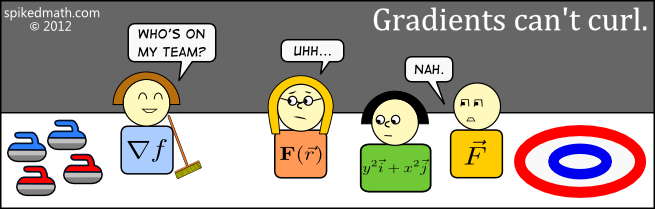
\includegraphics[width=10cm]{501-curling-with-gradients.png}
        \else
            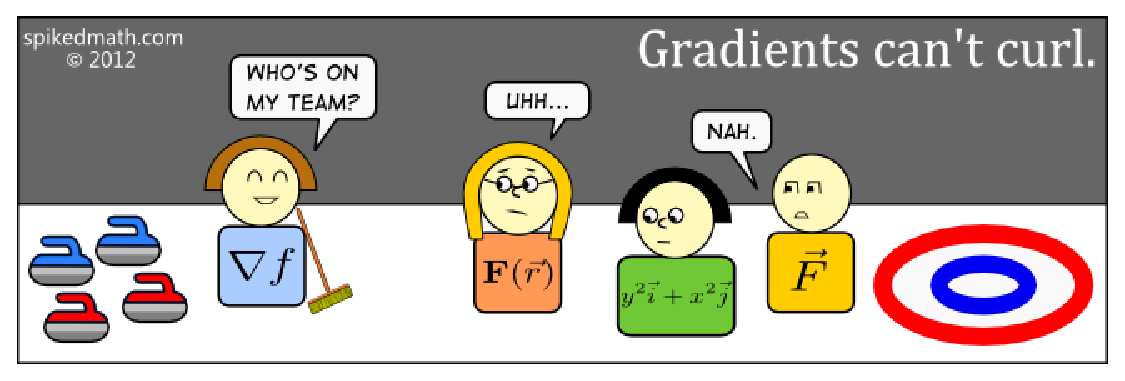
\includegraphics[width=10cm]{501-curling-with-gradients.eps}
        \fi

        {\tiny De \href{http://spikedmath.com/501.html}{Spiked math}, publié sous \href{http://creativecommons.org/licenses/by-nc-sa/2.5/ca/}{licence Creative Commons}.}
\end{center}

%+++++++++++++++++++++++++++++++++++++++++++++++++++++++++++++++++++++++++++++++++++++++++++++++++++++++++++++++++++++++++++
\section[Interprétation de la divergence]{Interprétation géométrique et physique de la divergence}
%+++++++++++++++++++++++++++++++++++++++++++++++++++++++++++++++++++++++++++++++++++++++++++++++++++++++++++++++++++++++++++

En physique, on dit qu'un champ de vecteurs à divergence nulle est \defe{incompressible}{incompressible!champ de vecteur}. Nous allons essayer de comprendre pourquoi. Lorsqu'un fluide incompressible se déplace, il faut qu'en chaque point il y autant de fluide qui rentre que de fluide qui sort. Nous allons voir sur quelque exemples que la divergence d'un champ de vecteurs est le «bilan de masse» d'un fluide qui se déplace selon le champ de vecteurs.

Si en un point la divergence est positive, cela signifie qu'il y a une perte de masse et si la divergence est négative, cela signifie qu'il y a une accumulation de masse.

Prenons par exemple un fluide qui se déplace selon le champ de vitesse montré à figure \ref{LabelFigBEHTooWsdrys}. % From file BEHTooWsdrys
\newcommand{\CaptionFigBEHTooWsdrys}{Le champ de vecteurs $F(x,y)=\frac{1}{ x }(1,0)$.}
\input{Fig_BEHTooWsdrys.pstricks}

Étant donné que la vitesse diminue lorsque $x$ avance, il y a une accumulation de fluide. Regardez en effet la quantité de fluide qui rentre dans le rectangle par rapport à la quantité de fluide qui en sort. Ce champ de vecteurs a pour équation :
\begin{equation}
    F(x,y)=\frac{1}{ x }\begin{pmatrix}
        1    \\ 
        0    
    \end{pmatrix}=\begin{pmatrix}
        1/x    \\ 
        0    
    \end{pmatrix}.
\end{equation}
Sa divergence vaut donc
\begin{equation}
    (\nabla\cdot F)(x,y)=\frac{ \partial F_x }{ \partial x }(x,y)+\underbrace{\frac{ \partial F_y }{ \partial y }(x,y)}_{=0}=-\frac{1}{ x^2 }.
\end{equation}
Cette divergence étant négative, il y a bien accumulation de fluide en tout point, et d'autant plus que $x$ est petit.

\begin{example}     \label{ExamDivFrot}

    Prenons le champ de vecteurs tournant
    \begin{equation}
        F(x,y)=\frac{1}{ \sqrt{x^2+y^2} }\begin{pmatrix}
            y    \\ 
            -x    
        \end{pmatrix}
    \end{equation}
    représenté à la figure \ref{LabelFigYQVHooYsGLHQ}. Cela est un vecteur qui est constamment perpendiculaire au rayon.


\newcommand{\CaptionFigYQVHooYsGLHQ}{Le champ de vecteurs $F(x,y)=(y,-x)$.}
\input{Fig_YQVHooYsGLHQ.pstricks}

    Un fluide dont la vitesse serait donné par ce champ de vecteur se contente de tourner. Intuitivement il ne devrait pas y avoir de divergence parce qu'il n'y a aucune accumulation de fluide. En effet,
    \begin{equation}
        \nabla\cdot F(x,y)=\frac{ -2xy }{ (x^2+y^2)^2 }+\frac{ 2xy }{ (x^2+y^2)^2 }=0.
    \end{equation}
\end{example}

\begin{example}
    Prenons le cas du champ de force de gravitation :
    \begin{equation}
        F(x,y,z)=\frac{1}{ (x^2+y^2+z^2)^{3/2} }\begin{pmatrix}
            x    \\ 
            y   \\
            z
        \end{pmatrix}.
    \end{equation}
    Nous pouvons rapidement remarquer que $\nabla\cdot F=0$. Est-ce que cela peut se comprendre sur le dessin de la figure \ref{LabelFigZGUDooEsqCWQ}. % From file ZGUDooEsqCWQ
\newcommand{\CaptionFigZGUDooEsqCWQ}{Le champ de vecteur de la gravité. Nous avons tracé, sur les deux cercles la même densité de vecteurs, c'est à dire le même nombre de vecteurs par unité de surface.}
\input{Fig_ZGUDooEsqCWQ.pstricks}

    Essayons de voir combien de fluide entre dans la zone bleue et combien en sort. D'abord, il est certain que les vecteurs qui sortent sont plus courts que ceux qui rentrent, ce qui voudrait dire qu'il y a plus de fluide qui rentre. Mais on voit également que le \emph{nombre} de vecteurs qui sortent est plus grand parce que la seconde sphère est plus grande et qu'il y a un vecteur en chaque point de la sphère.

    Intuitivement nous pouvons dire que la quantité qui rentre dans la sphère de rayon $r_1$ donnée par la taille des vecteurs entrants multiplié par la surface de la sphère, c'est à dire
    \begin{equation}        \label{EqQpinormeVecto}
        4\pi r_1^2\| F(x,y,z) \|,
    \end{equation}
    mais $\| F(x,y,z) \|=\frac{1}{ r_1^2 }$, donc la quantité de fluide entrant est $4\pi$. La quantité de fluide sortant sera la même.

    Cela explique deux choses
    \begin{enumerate}
        \item
            Pourquoi les forces de gravitation et électromagnétiques sont en $1/r^2$; c'est parce que nous vivons dans un monde avec trois dimensions d'espace. En étudiant très précisément le champ de gravitation, certains physiciens espèrent trouver des déviations expérimentales par rapport à la règle du \( 1/r^2\); cela \emph{pourrait} être un signe que l'espace contient des dimensions supplémentaires.
        \item
            Pourquoi il y a un $4\pi$ comme coefficient dans beaucoup d'équations en électromagnétisme; en particulier dans certaines anciennes unités de flux.
    \end{enumerate}
    
\end{example}

\begin{remark}
    Nous allons voir plus loin comment s'assurer que l'équation \eqref{EqQpinormeVecto} représente bien la «quantité de fluide» qui rentre dans la zone délimitée
\end{remark}


%+++++++++++++++++++++++++++++++++++++++++++++++++++++++++++++++++++++++++++++++++++++++++++++++++++++++++++++++++++++++++++
\section{Quelque formules de Leibnitz}
%+++++++++++++++++++++++++++++++++++++++++++++++++++++++++++++++++++++++++++++++++++++++++++++++++++++++++++++++++++++++++++

La divergence étant une combinaison de dérivées, il n'est pas tellement étonnant que la divergence de produits donne lieux à des formules en deux termes. Si $f$ est une fonction et si $F$ et $G$ sont des champs de vecteurs, nous avons (sans démonstrations) :
\begin{equation}        \label{EqLeinDivNablRot}
    \begin{aligned}[]
        \nabla\cdot(fF)&=f\nabla\cdot F+F\cdot\nabla f\\
        \nabla\cdot(F\times G)&=G\cdot\nabla\times F-F\cdot\nabla\times G.
    \end{aligned}
\end{equation}
Nous avons aussi, pour le rotationnel,
\begin{equation}        \label{EqLeinRotfFF}
    \nabla\times(fF)=f\nabla\times F+\nabla f\times F.
\end{equation}
% This is part of Mes notes de mathématique
% Copyright (c) 2011-2012
%   Laurent Claessens
% See the file fdl-1.3.txt for copying conditions.

%+++++++++++++++++++++++++++++++++++++++++++++++++++++++++++++++++++++++++++++++++++++++++++++++++++++++++++++++++++++++++++
\section{La différentielle revisitée}
%+++++++++++++++++++++++++++++++++++++++++++++++++++++++++++++++++++++++++++++++++++++++++++++++++++++++++++++++++++++++++++

%---------------------------------------------------------------------------------------------------------------------------
\subsection{Les formes différentielles de base}
%---------------------------------------------------------------------------------------------------------------------------

Si la fonction $f\colon \eR^n\to \eR$ est différentiable alors la différentielle en $a\in\eR^n$ est l'application
\begin{equation}        \label{EqFormDiffdfah}
    \begin{aligned}
        df_a\colon \eR^n&\to \eR \\
        u&\mapsto \frac{ \partial f }{ \partial x_1 }(a)u_1+\ldots+\frac{ \partial f }{ \partial x_n }(a)u_n.
    \end{aligned}
\end{equation}
Considérons en particulier la fonction qui à $x\in\eR^n$ fait correspondre $x_i\in\eR$. Par abus de notations,  nous la noterons $x_i$. Nous avons 
\begin{equation}
    \frac{ \partial x_i }{ \partial x_j }=\delta_{ij}.
\end{equation}
Par exemple $\partial_yx=0$ et $\partial_xx=1$. Toutes les dérivées partielles de $x_i$ s'annulent sauf la $i$ème qui vaut $1$. Par conséquent
\begin{equation}
    \begin{aligned}
        dx_i\colon \eR^n&\to \eR \\
        u&\mapsto u_i. 
    \end{aligned}
\end{equation}

\begin{remark}
    En toute rigueur nous devrions écrire $(dx_i)_a$. Mais étant donné que
    \begin{equation}
        (dx_i)_a(u)=(dx_i)_b(u)
    \end{equation}
    pour tout points $a$, $b$ et pour tout vecteurs $u$, nous nous permettons de simplifier la notation en ne précisant pas en quel point nous calculons la différentielle de $x_i$.
\end{remark}

Étant donné que $dx_i(u)=u_i$, nous pouvons récrire la formule \eqref{EqFormDiffdfah} en remplaçant $u_i$ par $dx_i(u)$ :
\begin{equation}
    df_a(u)=\frac{ \partial f }{ \partial x_1 }(a)dx_1(u)+\ldots+\frac{ \partial f }{ \partial x_n }(a)dx_n(u).
\end{equation}
En tant que application linéaire, $df_a$ est une combinaison linéaire des $dx_i$. En notations compacte :
\begin{equation}
    df_a=\sum_{i=1}^n\frac{ \partial f }{ \partial x_i }(a)dx_i.
\end{equation}

%---------------------------------------------------------------------------------------------------------------------------
\subsection{Différentielles de fonctions composées}
%---------------------------------------------------------------------------------------------------------------------------

Cette façon de voir la différentielle nous permet de jeter un nouveau regard sur la formule de différentiation des fonctions composées. Soient
\begin{equation}
    \begin{aligned}[]
        f\colon \eR^p&\to \eR^n\\
        g\colon \eR^n&\to \eR,
    \end{aligned}
\end{equation}
et $h\colon \eR^p\to \eR$ définie par 
\begin{equation}
    h(u)=h\big( f(u) \big)=(g\circ f)(u).
\end{equation}
Nous allons noter $x$ les coordonnées de $\eR^p$, $a$ un point de $\eR^p$ et $u$, un vecteur de $\eR^p$ accroché au point $a$. Pour $\eR^n$, les notations seront que les coordonnées sont $y$, $b$ est un point de $\eR^n$ et $v$ est un vecteur «accroché» au point $b$.

Nous avons
\begin{equation}
    dg_b(v)=\sum_{i=1}^n\frac{ \partial g }{ \partial y_i }(b)dy_i(v).
\end{equation}
Ici $dy_i(v)$ signifie la $i$ème composante de $v$. C'est simplement $v_i$. Cette formule étant valable pour tout point $b\in\eR^n$ et pour tout vecteur $v$, nous pouvons l'écrire en particulier pour
\begin{subequations}
    \begin{numcases}{}
        b=f(a)\\
        v=df_a(u).
    \end{numcases}
\end{subequations}
Cela donne
\begin{equation}        \label{Eqdgfadfau}
    dg_{f(a)}\big( df_a(u) \big)=\sum_{i=1}^n\frac{ \partial g }{ \partial y_i }\big( f(a) \big)dy_i\big( df_a(u) \big).
\end{equation}
Mais 
\begin{equation}
    df_a(u)=\sum_{j=1}^p\frac{ \partial f }{ \partial x_j }(a)dx_j(u),
\end{equation}
donc la $i$ème composante de ce vecteur est
\begin{equation}
     \big( df_a(u)\big)_i=\sum_{j=1}^p\frac{ \partial f_i }{ \partial x_j }(a)dx_j(u).
\end{equation}
En remplaçant $dy_i\big( df_a(u) \big)$ par cela dans l'expression \eqref{Eqdgfadfau}, nous trouvons
\begin{equation}
    dg_{f(a)}\big( df_a(u) \big)=\sum_{i=1}^n\frac{ \partial g }{ \partial y_i }\big( f(a) \big)\sum_{j=1}^p\frac{ \partial f_i }{ \partial x_j }(a)dx_j(u).
\end{equation}
Nous pouvons vérifier que cela est la différentielle de $g\circ f$ au point $a$ appliquée au vecteur $u$. En effet
\begin{equation}
    d(g\circ f)_a(u)=\sum_{j=1}^p\frac{ \partial (g\circ f) }{ \partial x_j }(a)dx_j(u),
\end{equation}
tandis que, par la dérivation de fonctions composées, 
\begin{equation}        \label{EqDerCompofg}
    \frac{ \partial (g\circ f) }{ \partial x_j }(a)=\sum_{i=1}^n\frac{ \partial g }{ \partial y_i }\big( f(a) \big)\frac{ \partial f_i }{ \partial x_j }(a).
\end{equation}
Au final, ce que nous avons prouvé est que
\begin{equation}
    d(g\circ f)_a(u)=dg_{f(a)}\big( df_a(u) \big).
\end{equation}

%---------------------------------------------------------------------------------------------------------------------------
\subsection{Passage aux coordonnées polaires}
%---------------------------------------------------------------------------------------------------------------------------

Le changement de coordonnées pour les polaires est la fonction
\begin{equation}
    f\begin{pmatrix}
        r    \\ 
        \theta    
    \end{pmatrix}=\begin{pmatrix}
        x    \\ 
        y    
    \end{pmatrix}=\begin{pmatrix}
        r\cos\theta    \\ 
        r\sin\theta    
    \end{pmatrix}.
\end{equation}
Considérons une fonction $g$ sur $\eR^2$, et définissons la fonction $\tilde g$ par
\begin{equation}
    \tilde g(r,\theta)=g(r\cos\theta,r\sin\theta).
\end{equation}
La formule \eqref{EqDerCompofg} permet de trouver les dérivées partielles de $g$ par rapport à $r$ et $\theta$ en termes de celles par rapport à $x$ et $y$ de $g$.

Pour faire le lien avec les notations du point précédent, nous avons
\begin{equation}
    \begin{aligned}[]
        f_1(r,\theta)&=r\cos(\theta)\\
        f_2(r,\theta)&=r\sin(\theta)\\
        (x_1,x_2)&\to(r,\theta)\\
        (y_1,y_2)&\to(x,y).
    \end{aligned}
\end{equation}
Nous avons donc 
\begin{equation}
    \begin{aligned}[]
        \frac{ \partial \tilde g }{ \partial r }(r,\theta)&=\sum_{i=1}^2\frac{ \partial g }{ \partial x_i }\big( f(r,\theta) \big)\frac{ \partial f_i }{ \partial r }(r,\theta)\\
        &=\frac{ \partial g }{ \partial x }(r\cos\theta,r\sin\theta)\frac{ \partial \big( r\cos\theta \big) }{ \partial r }(r,\theta)\\
        &\quad+\frac{ \partial g }{ \partial y }(r\cos\theta,r\sin\theta)\frac{ \partial \big( r\sin\theta\big) }{ \partial r }(r,\theta)\\
        &=\cos\theta\frac{ \partial g }{ \partial x }(r\cos\theta,r\sin\theta)+\sin\theta\frac{ \partial g }{ \partial y }(r\cos\theta,r\sin\theta).
    \end{aligned}
\end{equation}

Prenons par exemple $g(x,y)=\frac{1}{ x^2+y^2 }$. Étant donné que
\begin{equation}
    \frac{ \partial g }{ \partial x }=\frac{ -2x }{ (x^2+y^2)^2 },
\end{equation}
nous avons
\begin{equation}
    \frac{ \partial g }{ \partial x }(r\cos\theta,r\sin\theta)=\frac{ -2\cos\theta }{ r^3 }.
\end{equation}
En utilisant la formule,
\begin{equation}
    \frac{ \partial \tilde g }{ \partial r }(r,\theta)=\cos(\theta)\left( \frac{ -2\cos\theta }{ r^3 } \right)+\sin(\theta)\left( \frac{ -2\sin\theta }{ r^3 } \right)=-\frac{ 2 }{ r^3 }.
\end{equation}
Nous pouvons vérifier directement que cela est correct. En effet
\begin{equation}
    \tilde g(r,\theta)=g(r\cos\theta,r\sin\theta)=\frac{1}{ r^2 },
\end{equation}
dont la dérivée par rapport à $r$ vaut $-2/r^3$.

En ce qui concerne la dérivée par rapport à $\theta$, nous avons
\begin{equation}
    \begin{aligned}[]
    \frac{ \partial \tilde g }{ \partial \theta }&=\frac{ \partial g }{ \partial x }(r\cos\theta,r\sin\theta)\frac{ \partial \big( r\cos(\theta) \big) }{ \partial \theta }+\frac{ \partial g }{ \partial y }(r\cos\theta,r\sin\theta)\frac{ \partial \big( r\sin(\theta) \big) }{ \partial \theta }\\
    &=\left( \frac{ -2\cos\theta }{ r^3 } \right)(-r\sin\theta)+\left( \frac{ -2\sin\theta }{ r^3 } \right)(r\cos\theta)\\
    &=0.
    \end{aligned}
\end{equation}

En résumé et avec quelque abus de notations :
\begin{equation}
    \begin{aligned}[]
        \frac{ \partial \tilde g }{ \partial r }&=\cos(\theta)\frac{ \partial g }{ \partial x }+\sin(\theta)\frac{ \partial g }{ \partial y }\\
        \frac{ \partial \tilde g }{ \partial \theta }&=-r\sin(\theta)\frac{ \partial g }{ \partial x }+r\cos(\theta)\frac{ \partial g }{ \partial y }\\
    \end{aligned}
\end{equation}

%+++++++++++++++++++++++++++++++++++++++++++++++++++++++++++++++++++++++++++++++++++++++++++++++++++++++++++++++++++++++++++
\section{Théorie générale}
%+++++++++++++++++++++++++++++++++++++++++++++++++++++++++++++++++++++++++++++++++++++++++++++++++++++++++++++++++++++++++++

%---------------------------------------------------------------------------------------------------------------------------
\subsection{Base locale}
%---------------------------------------------------------------------------------------------------------------------------

Les coordonnées sphériques et cylindriques sont deux systèmes de coordonnées «un peu courbe» qui existent sur $\eR^3$. Il en existe de nombreux autres, que nous appelons \defe{coordonnées curvilignes}{coordonnées!curvilignes}. Des coordonnées curvilignes sur $\eR^3$ est n'importe quel\footnote{Nous n'entrons pas dans les détails de régularité.} système qui permet de repérer un point de $\eR^3$ à partir de trois nombres.

Il s'agit donc d'un ensemble de trois applications 
\begin{equation}
    x_i\colon \eR^3\to \eR.
\end{equation}
Les coordonnées cylindriques sont
\begin{subequations}
    \begin{numcases}{}
        x_1(r,\theta,z)=r\cos\theta\\
        x_2(r,\theta,z)=r\sin\theta\\
        x_3(r,\theta,z)=z
    \end{numcases}
\end{subequations}

Soit donc un système général $q=(q_1,q_2,q_3)$ et 
\begin{equation}
    M(q)=\begin{pmatrix}
        x_1(q)    \\ 
        x_2(q)    \\ 
        x_3(q)    
    \end{pmatrix}.
\end{equation}
Si nous fixons $q_2$ et $q_3$ et que nous laissons varier $q_1$, nous obtenons une courbe\footnote{Dans le cas des sphériques, c'est une demi-droite horizontale d'angle $q_2$ et de hauteur $q_3$.} dont nous pouvons considérer le vecteur vitesse, c'est à dire le vecteur tangent. En chaque point nous avons ainsi trois vecteurs
\begin{equation}
    \frac{ \partial M }{ \partial q_i }(q).
\end{equation}
Nous disons que le système de coordonnées curviligne est \defe{orthogonal}{orthogonal!coordonnées curviligne} si ces trois vecteurs sont orthogonaux. Dans la suite nous supposerons que c'est toujours le cas.

Nous posons
\begin{equation}
    h_i=\left\| \frac{ \partial M }{ \partial q_i } \right\|
\end{equation}
et nous considérons les trois vecteurs normés
\begin{equation}        \label{EqDefeihMq}
    e_i=h_i^{-1}\frac{ \partial M }{ \partial q_i }.
\end{equation}
Les trois vecteurs $\{ e_1,e_2,e_3 \}$ forment une base orthonormée dite \defe{base locale}{base!locale}. Ce sont des vecteurs liés\footnote{En géométrie différentielle on dira que ce sont des élément de l'espace tangent, mais c'est une toute autre histoire.} au point $M$.

%---------------------------------------------------------------------------------------------------------------------------
\subsection{Importance de l'orthogonalité}
%---------------------------------------------------------------------------------------------------------------------------

Nous avons dit que nous nous restreignons au cas où les vecteurs $e_i$ sont orthogonaux. En termes de produits scalaires, cela signifie
\begin{equation}
    e_i\cdot e_j=\delta_{ij}.
\end{equation}
Nous en étudions maintenant quelque conséquence. L'équation \eqref{EqDefeihMq} peut s'écrire plus explicitement sous la forme
\begin{equation}
    e_i=\sum_k h_i^{-1}\frac{ \partial x_k }{ \partial q_i }1_k.
\end{equation}
Notez que pour chaque $k$ et $i$, la quantité $h_i^{-1}\frac{ \partial x_k }{ \partial q_i }$ est un simple nombre. Nous allons les mettre dans une matrice :
\begin{equation}
    A_{ki}=h_i^{-1}\frac{ \partial x_k }{ \partial q_i }.
\end{equation}
Cela nous donne le changement de base
\begin{equation}        \label{EqChmBaseeisAkiAk}
    e_i=\sum_kA_{ki}1_k.
\end{equation}
Le produit $e_i\cdot e_j$ s'écrit alors
\begin{equation}
    \begin{aligned}[]
        e_i\cdot e_j&=\sum_{kl}A_{ki}A_{lj}\underbrace{1_k\cdot 1_l}_{=\delta_{kl}}\\
        &=\sum_{kl}A_{ki}A_{lj}\delta_{kl}\\
        &=\sum_kA_{ki}A_{kj}\\
        &=\sum_k(A^T)_{ik}A_{kj}.
    \end{aligned}
\end{equation}
Or cela doit valoir $\delta_{ij}$. Par conséquent 
\begin{equation}
    A^T=A^{-1}.
\end{equation}
Le fait que les coordonnées curvilignes considérées soient orthogonales s'exprime donc par la fait que la matrice de changement de base est une matrice orthogonale.

Cette circonstance nous permet d'inverser le changement de base \eqref{EqChmBaseeisAkiAk} en multipliant cette équation par $(A^{-1})_{il}$ des deux côtés et en faisant la somme sur $i$ :
\begin{equation}
    \sum_i (A^{-1})_{il}e_i=\sum_{kl}\underbrace{A_{ki}(A^{-1})_{il}}_{=\delta_{kl}}1_k,
\end{equation}
par conséquent
\begin{equation}
    \sum_i(A^T)_{il}e_i=1_l,    
\end{equation}
et
\begin{equation}        \label{EqChamvarunlAei}
    1_l=\sum_iA_{li}e_i=\sum_ih_i^{-1}\frac{ \partial x_l }{ \partial q_i }e_i.
\end{equation}
Armés de cette importante formule, nous pouvons exprimer les quantités que nous connaissons dans la base canonique en termes de la base locale.

Une autre conséquence du fait que $e_1$, $e_2$ et $e_3$ est une base orthonormée est que, éventuellement en réordonnant les vecteurs, on a
\begin{equation}
    \begin{aligned}[]
        e_1\times e_2&=e_3\\
        e_2\times e_3&=e_1\\
        e_3\times e_1&=e_2
    \end{aligned}
\end{equation}
Ces trois relations s'écrivent en une seule avec
\begin{equation}
    e_i\times e_j=\sum_{k}\epsilon_{ijk}e_k
\end{equation}
où 
\begin{equation}
    \epsilon_{ijk}=\begin{cases}
        0    &   \text{si $i$, $j$ et $k$ ne sont pas tous différents}\\
        1    &    \text{si $ijk$ se ramène à $123$ par un nombre pair de permutations}\\
        -1    &    \text{si $ijk$ se ramène à $123$ par un nombre impair de permutations}
    \end{cases}
\end{equation}
est le \defe{symbole de Levi-Civita}{Levi-Civita}. La formule du produit vectoriel peut également être utilisée à l'envers sous la forme
\begin{equation}        \label{Eqekeitimesej}
    e_k=\frac{ 1 }{2}\sum_{ij}\epsilon_{ijk}\,e_i\times e_j.
\end{equation}

Le symbole de Levi-Civita possède de nombreuses formules. En voici certaines, facilement démontrables en considérant tous les cas :
\begin{equation}
    \epsilon_{ijk}\epsilon_{ijl}=\delta_{kl}| \epsilon_{ijk} |.
\end{equation}
Grâce au symboles de Levi-Civita, le produit mixte des vecteurs de base a une belle forme :
\begin{equation}        \label{EqProdMixteepsilonCicivr}
    e_l\cdot(e_i\times e_j)=\sum_k\epsilon_{ijk}e_l\times e_k=\sum_k\epsilon_{ijk}\delta_{lk}=\epsilon_{ijl}.
\end{equation}

%+++++++++++++++++++++++++++++++++++++++++++++++++++++++++++++++++++++++++++++++++++++++++++++++++++++++++++++++++++++++++++
\section{Gradient en coordonnées curvilignes}
%+++++++++++++++++++++++++++++++++++++++++++++++++++++++++++++++++++++++++++++++++++++++++++++++++++++++++++++++++++++++++++

Soit $(x,y,z)\mapsto f(x,y,z)$ une fonction sur $\eR^3$. Nous pouvons la composer avec les coordonnées curvilignes $q$ pour obtenir la fonction
\begin{equation}
    \tilde f(q_1,q_2,q_3)=f\big( x_1(q),x_2(x),x_3(q) \big).
\end{equation}
Nous disons que $\tilde f$ est l'expression de $f$ dans les coordonnées $q$. Nous savons déjà comment calculer le gradient de $f$ en coordonnées cartésiennes :
\begin{equation}
    F(x,y, z)=\nabla f(x,y,z)=\begin{pmatrix}
        \partial_xf(x,y,z)    \\ 
        \partial_yf(x,y,z)    \\ 
        \partial_zf(x,y,z)    \
    \end{pmatrix}.
\end{equation}
Cela est un vecteur lié au point $(x,y,z)$. Nous voudrions exprimer ce vecteur dans la base $\{ e_1,e_2,e_3 \}$. En d'autres termes, nous voudrions trouver les nombres $\tilde F_1$, $\tilde F_2$ et $\tilde F_3$ tels que
\begin{equation}
    F(x,y,z)=F\big( x(q),y(q),z(q) \big)=\tilde F_1e_1+\tilde F_2e_2+\tilde F_3e_3.
\end{equation}
Ces nombres seront des fonctions de $(q_1,q_2,q_3)$.

Par définition,
\begin{equation}
    \nabla f=\sum_l\frac{ \partial f }{ \partial x_l }1_l.
\end{equation}
En remplaçant $1_l$ par sa valeur en termes des $e_i$ par la formule \eqref{EqChamvarunlAei},
\begin{equation}
    \begin{aligned}[]
        \nabla f&=\sum_l\frac{ \partial f }{ \partial x_l }1_l\\
        &=\sum_l\frac{ \partial f }{ \partial x_l }\sum_ih_i^{-1}\frac{ \partial x_l }{ \partial q_i }e_i\\
        &=\sum_{il}\frac{1}{ h_i }\frac{ \partial f }{ \partial x_l }\frac{ \partial x_l }{ \partial q_i }e_i\\
        &=\sum_i\frac{1}{ h_i }\frac{ \partial \tilde f }{ \partial q_i }e_i.
    \end{aligned}
\end{equation}

Plus explicitement,
\begin{equation}        \label{EqGradientenCurviligne}
    \nabla f\big( x(q),y(q),z(q) \big)=\sum_i \frac{1}{ h_i(q) }\frac{ \partial \tilde f }{ \partial q_i }(q)e_i
\end{equation}
où
\begin{equation}
    h_i(q)=\left\| \frac{ \partial M }{ \partial q_i }(q) \right\|.
\end{equation}
Le plus souvent nous n'allons pas noter explicitement la dépendance de $h_i$ en $q$.

Quelque formulaires intéressants sont en appendice de \cite{Schomblond_em}.

%---------------------------------------------------------------------------------------------------------------------------
\subsection{Coordonnées polaires}
%---------------------------------------------------------------------------------------------------------------------------

Les coordonnées curvilignes polaires sont données par
\begin{equation}
    M(r,\theta)=\begin{pmatrix}
        r\cos(\theta)    \\ 
        r\sin(\theta)    
    \end{pmatrix},
\end{equation}
et par conséquent
\begin{equation}
    \begin{aligned}[]
        \frac{ \partial M }{ \partial r }&=\begin{pmatrix}
            \cos(\theta)    \\ 
            \sin(\theta)    
        \end{pmatrix},&\frac{ \partial M }{ \partial \theta }=\begin{pmatrix}
            -r\sin(\theta)    \\ 
            r\cos(\theta)    
        \end{pmatrix}.
    \end{aligned}
\end{equation}
Nous avons les normes $h_r=1$ et $h_{\theta}=r$, et donc les vecteurs de la base locale en $(r,\theta)$ sont
\begin{equation}
    e_r=\begin{pmatrix}
        \cos(\theta)    \\ 
        \sin(\theta)    
    \end{pmatrix}=\cos(\theta)e_x+\sin(\theta)e_y
\end{equation}
ainsi que
\begin{equation}
    e_{\theta}=\begin{pmatrix}
        -\sin(\theta)    \\ 
        \cos(\theta)    
    \end{pmatrix}=-\sin(\theta)e_x+\cos(\theta)e_y.
\end{equation}


Ces vecteurs sont représentés à la figure \ref{LabelFigHGQPooKrRtAN}. Notez qu'il y en a une paire différente en chaque point.
\newcommand{\CaptionFigHGQPooKrRtAN}{En brun, les lignes que le point suivrait si on ne variait qu'une coordonnées polaire à la fois. Les vecteurs rouges sont les vecteurs $e_{r}$ et $e_{\theta}$.}
\input{Fig_HGQPooKrRtAN.pstricks}

%---------------------------------------------------------------------------------------------------------------------------
\subsection{Coordonnées cylindriques}
%---------------------------------------------------------------------------------------------------------------------------

Les coordonnées cylindriques sont les mêmes que les coordonnées polaires à part qu'il faut écrire
\begin{equation}
    M(r,\theta,z)=\begin{pmatrix}
        r\cos(\theta)    \\ 
        r\sin(\theta)    \\ 
        z    
    \end{pmatrix},
\end{equation}
et nous avons le vecteur de base supplémentaire
\begin{equation}
    e_z=\frac{ \partial M }{ \partial z }=\begin{pmatrix}
        0    \\ 
        0    \\ 
        1    
    \end{pmatrix}
\end{equation}
parce que $h_z=1$.

%---------------------------------------------------------------------------------------------------------------------------
\subsection{Coordonnées sphériques}
%---------------------------------------------------------------------------------------------------------------------------

Les coordonnées curvilignes sphériques sont données par
\begin{equation}
    M(\rho,\theta,\varphi)=
    \begin{pmatrix}
        \rho\sin(\theta)\cos(\varphi)    \\ 
        \rho\sin(\theta)\sin(\varphi)    \\ 
        \rho\cos(\theta)
    \end{pmatrix},
\end{equation}
dont les dérivées sont données par
\begin{equation}
    \begin{aligned}[]
        \frac{ \partial M }{ \partial r }&=\begin{pmatrix}
        \sin(\theta)\cos(\varphi)    \\ 
        \sin(\theta)\sin(\varphi)    \\ 
        \cos(\theta)
    \end{pmatrix},
    &\frac{ \partial M }{ \partial \theta }&=
    \begin{pmatrix}
        \rho\cos(\theta)\cos(\varphi)    \\ 
        \rho\cos(\theta)\sin(\varphi)    \\ 
        -\rho\sin(\theta)
    \end{pmatrix},\\
    \frac{ \partial M }{ \partial \varphi }&=
    \begin{pmatrix}
        -\rho\sin(\theta)\sin(\varphi)    \\ 
        \rho\sin(\theta)\cos(\varphi)    \\ 
        0
    \end{pmatrix}
    \end{aligned}
\end{equation}
Les normes de ces vecteurs sont $h_{\rho}=1$, $h_{\theta}=\rho$ et $h_{\varphi}=\rho\sin(\theta)$. Les vecteurs de la base locale en $(\rho,\theta,\varphi)$ sont donc
\begin{equation}
    \begin{aligned}[]
        e_r&=\begin{pmatrix}
        \sin(\theta)\cos(\varphi)    \\ 
        \sin(\theta)\sin(\varphi)    \\ 
        \cos(\theta)
    \end{pmatrix},
    &e_{\theta}&=
    \begin{pmatrix}
        \cos(\theta)\cos(\varphi)    \\ 
        \cos(\theta)\sin(\varphi)    \\ 
        -\sin(\theta)
    \end{pmatrix},\\
    e_{\varphi}&=
    \begin{pmatrix}
        -\sin(\varphi)    \\ 
        \cos(\varphi)    \\ 
        0
    \end{pmatrix}
    \end{aligned}
\end{equation}

Nous pouvons exprimer le gradient d'une fonction en coordonnées sphériques en utilisant la formule \eqref{EqGradientenCurviligne} :
\begin{equation}        \label{EqGradientSpherique}
    \nabla\tilde f(\rho,\theta,\varphi)=\frac{ \partial \tilde f }{ \partial \rho }e_{\rho}+\frac{1}{ \rho }\frac{ \partial \tilde f }{ \partial \theta }e_{\theta}+\frac{1}{ \rho\sin(\theta) }\frac{ \partial \tilde f }{ \partial \varphi }r_{\varphi}.
\end{equation}
Cette expression peut paraître peu pratique parce que les vecteurs $e_{\rho}$, $e_{\theta}$ et $e_{\varphi}$ eux-mêmes changent en chaque point. Elle est effectivement peu adaptée au dessin, mais elle est très pratique pour des fonctions ayant des symétries.

\begin{example}
    Le potentiel de la gravitation est la fonction
    \begin{equation}
        V(x,y,z)=\frac{1}{ \sqrt{x^2+y^2+z^2} }.
    \end{equation}
    En coordonnées sphériques elle s'écrit
    \begin{equation}
        \tilde V(\rho,\theta,\varphi)=\frac{1}{ \rho }.
    \end{equation}
    En voila une fonction qu'elle est facile à dériver, contrairement à $V$ ! En suivant la formule \eqref{EqGradientSpherique}, nous avons immédiatement
    \begin{equation}
        \nabla\tilde V=-\frac{1}{ \rho^2 }e_{\rho}.
    \end{equation}
    Nous voyons immédiatement que cela est un champ de vecteurs dont la norme diminue comme le carré de la distance à l'origine et qui est en permanence dirigé vers l'origine.
\end{example}


%+++++++++++++++++++++++++++++++++++++++++++++++++++++++++++++++++++++++++++++++++++++++++++++++++++++++++++++++++++++++++++
\section{Divergence en coordonnées curvilignes}
%+++++++++++++++++++++++++++++++++++++++++++++++++++++++++++++++++++++++++++++++++++++++++++++++++++++++++++++++++++++++++++

Nous savons que 
\begin{equation}
    \nabla\tilde f=\sum_j\frac{1}{ h_j }\frac{ \partial \tilde f }{ \partial q_j }e_j.
\end{equation}
Nous pouvons en particulier considérer la fonction $f(q)=q_i$. De la même manière que nous avions noté $x_i$ la fonction $x\mapsto x_i$, nous notons $q_i$ la fonction $q\mapsto q_i$. Le gradient de cette fonction est donné par
\begin{equation}
    \nabla q_i=\sum_j\frac{1}{ h_j }\frac{ \partial q_i }{ \partial q_j }e_j,
\end{equation}
mais $\frac{ \partial q_i }{ \partial q_j }=\delta_{ij}$, donc
\begin{equation}
    \nabla q_i=\frac{ e_i }{ h_i },
\end{equation}
ou encore
\begin{equation}
    e_i=h_i\nabla q_i.
\end{equation}
Cela n'est pas étonnant : la direction dans laquelle la coordonnées $q_i$ varie le plus est le vecteur $e_i$ qui donne la tangente à la courbe obtenue lorsque \emph{seul} $q_i$ varie.

Commençons par calculer la divergence de $e_i$. En utilisant la formule \eqref{Eqekeitimesej},
\begin{equation}
    \nabla\cdot e_k=\frac{ 1 }{2}\sum_{ij}\epsilon_{ijk}\,\nabla\cdot (e_i\times e_j).
\end{equation}
Nous avons, en utilisant les règles de Leibnitz \eqref{EqLeinDivNablRot}, 
\begin{equation}
    \begin{aligned}[]
        \nabla\cdot(e_i\times e_j)&=\nabla\cdot(h_i\nabla q_i\times h_j\nabla q_j)\\
        &=\nabla(h_ih_j)\cdot\big( \nabla q_i\times\nabla q_j \big)+h_ih_j\nabla\cdot\big( \nabla q_i\times\nabla q_j \big)\\
        &=\nabla(h_ih_j)\cdot\big( \nabla q_i\times\nabla q_j \big)\\
        &\quad+h_ih_j\nabla q_j\cdot\big( \underbrace{\nabla\times\nabla q_i}_{=0} \big)\\
        &\quad+h_ih_j\nabla q_i\cdot\big( \underbrace{\nabla\times\nabla q_j}_{=0} \big)
    \end{aligned}
\end{equation}
Cela nous fait
\begin{equation}
    \nabla\cdot e_k=\sum_{ij}\epsilon_{ijk}\frac{ \nabla(h_ih_j) }{ h_ih_j }\cdot (e_i\times e_j).
\end{equation}
parce que $\nabla q_i=h_i^{-1}e_i$. Nous pouvons développer le gradient qui intervient :
\begin{equation}
    \nabla(h_ih_j)=\sum_l\frac{1}{ h_l }\frac{ \partial  }{ \partial q_l }(h_ih_j)e_l.
\end{equation}
Nous voyons donc arriver le produit mixte $e_l\cdot (e_i\times e_j)$. En utilisant la formule \eqref{EqProdMixteepsilonCicivr}, cela s'exprime directement sous la forme $\epsilon_{ijl}$.

Nous avons alors
\begin{equation}        \label{EqFragradekdvi}
    \begin{aligned}[]
        \nabla\cdot e_k&=\frac{ 1 }{2}\sum_{ijl}\frac{1}{ h_ih_jh_l }\frac{ \partial  }{ \partial q_l }(h_ih_j)\epsilon_{ijk}\epsilon_{ijl}\\
        &=\frac{ 1 }{2}\sum_{ijl}\delta_{kl}| \epsilon_{ijk} |\frac{ \partial  }{ \partial q_l }(h_ih_j)\\
        &=\frac{ 1 }{2}\sum_{ij}\frac{| \epsilon_{ijk} |}{ h_ih_jh_k }\frac{ \partial  }{ \partial q_k }(h_ih_j).
    \end{aligned}
\end{equation}
Par exemple,
\begin{equation}
    \nabla\cdot e_1=\frac{1}{ h_1h_2h_3 }\frac{ \partial  }{ \partial q_1 }(h_2h_3).
\end{equation}

Nous devons maintenant chercher le gradient d'un champ général
\begin{equation}
    F(q)=\sum_kF_k(q)e_k.
\end{equation}
La première chose à faire est d'utiliser la formule de Leibnitz :
\begin{equation}        \label{EqLeibnbablaFek}
    \nabla\cdot F=\sum_k\nabla F_k(q)\cdot e_k+\sum_kF_k(q)\nabla\cdot e_k.
\end{equation}
Afin d'alléger les notations, nous allons nous concentrer sur le terme numéro $k$ et ne pas écrire la somme. Si $i$ et $j$ sont les nombres tels que $\epsilon_{ijk}=1$, alors ce que la formule \eqref{EqFragradekdvi} signifie, c'est que
\begin{equation}
    \nabla\cdot e_k=\frac{1}{ h_1h_2h_3 }\frac{ \partial  }{ \partial q_k }(h_ih_j).
\end{equation}
Nous savons déjà par la formule \eqref{EqGradientenCurviligne} que
\begin{equation}
    \nabla F_k=\sum_l\frac{1}{ h_l }\frac{ \partial F_k }{ \partial q_l }e_l,
\end{equation}
par conséquent
\begin{equation}
    \nabla F_k\cdot e_k=\sum_l\frac{1}{ h_l }\frac{ \partial F_k }{ \partial q_l }\delta_{kl}=\frac{1}{ h_k }\frac{ \partial F_k }{ \partial q_k }.
\end{equation}
Pour obtenir cela nous avons utilisé le fait que $e_l\cdot e_k=\delta_{lk}$. Le terme numéro $k$ de la somme \eqref{EqLeibnbablaFek} est donc
\begin{equation}
    \frac{1}{ h_k }\frac{ \partial F_k }{ \partial q_k }+\frac{ F_k }{ h_kh_ih_j }\frac{ \partial (h_ih_j) }{ \partial q_k }=\frac{1}{ h_ih_jh_k }\frac{ \partial (F_kh_ih_j) }{ \partial q_k }
\end{equation}
où il est entendu que $i$ et $j$ représentent les nombres tels que $\epsilon_{ijk}=1$.

Au final, nous avons
\begin{equation}
    \nabla\cdot F=\frac{1}{ h_1h_2h_3 }\sum_{ijk}| \epsilon_{ijk} |\frac{ \partial (F_kh_ih_j) }{ \partial q_k }.
\end{equation}
Ici, la somme sur $i$ et $j$ consiste seulement à sélectionner les termes tels que $i$ et $j$ ne sont pas $k$. En écrivant la somme explicitement,
\begin{equation}
    \begin{aligned}[]
        \nabla\cdot F=\frac{1}{ h_1h_2h_3 }\left[ \frac{ \partial  }{ \partial q_1 }(F_1h_2h_3)+\frac{ \partial  }{ \partial q_2 }(F_2h_1h_3)+\frac{ \partial  }{ \partial q_3 }(F_3h_1h_2) \right].
    \end{aligned}
\end{equation}

%---------------------------------------------------------------------------------------------------------------------------
\subsection{Coordonnées cylindriques}
%---------------------------------------------------------------------------------------------------------------------------

En coordonnées cylindriques, nous avons déjà vu que $h_r=1$, $h_{\theta}=r$ et $h_z=1$. La divergence est donc donnée par
\begin{equation}        \label{EqDivEnCylonf}
    \nabla\cdot F=\frac{1}{ r }\left[ \frac{ \partial  }{ \partial r }(rF_r)+\frac{ \partial  }{ \partial \theta }(F_{\theta})+\frac{ \partial  }{ \partial z }(rF_z) \right].
\end{equation}
Par exemple si
\begin{equation}
    F(r,\theta,z)=re_{\theta}+e_z,
\end{equation}
nous avons
\begin{equation}
    (\nabla\cdot F)(r,\theta,z)=\frac{1}{ r }\left[ \frac{ \partial  }{ \partial \theta }(r)+\frac{ \partial  }{ \partial z }(r) \right]=0.
\end{equation}
Cela est logique parce que $re_{\theta}$ est à peu près le champ dont nous avons parlé dans l'exemple \eqref{ExamDivFrot}, qui était à divergence nulle. En réalité, le champ dont on parlait dans cet exemple était exactement $-e_{\theta}$. Le champ $e_z$ est également à divergence nulle parce qu'il est constant.

%---------------------------------------------------------------------------------------------------------------------------
\subsection{Coordonnées sphériques}
%---------------------------------------------------------------------------------------------------------------------------

En coordonnées sphériques, nous avons $h_{\rho}=1$, $h_{\theta}=r$ et $h_{\varphi}=r\sin\theta$, donc
\begin{equation}
    \nabla\cdot F=\frac{1}{ r^2\sin\theta }\left[ \frac{ \partial  }{ \partial \rho }(\rho^2\sin\theta F_{\rho})+\frac{ \partial  }{ \partial \theta }(\rho\sin\theta F_{\theta})+\frac{ \partial  }{ \partial \varphi }(\rho F_{\varphi}) \right].
\end{equation}
si $F(\rho,\theta,\varphi)=F_{\rho}e_{\rho}+F_{\theta}e_{\theta}+F_{\varphi}e_{\varphi}$.

%+++++++++++++++++++++++++++++++++++++++++++++++++++++++++++++++++++++++++++++++++++++++++++++++++++++++++++++++++++++++++++
\section{Laplacien en coordonnées curvilignes orthogonales}
%+++++++++++++++++++++++++++++++++++++++++++++++++++++++++++++++++++++++++++++++++++++++++++++++++++++++++++++++++++++++++++

Soit une fonction $f\colon \eR^3\to \eR$. Le \defe{Laplacien}{Laplacien} de $f$ est donné par
\begin{equation}
    \Delta f=\nabla\cdot(\nabla f).
\end{equation}
En utilisant les formules données, nous avons
\begin{equation}
    \Delta f=\frac{1}{ h_1h_2h_3 }\left[ \frac{ \partial  }{ \partial q_1 }\left( \frac{ h_2h_3 }{ h_1 }\frac{ \partial f }{ \partial q_1 } \right)  +\frac{ \partial  }{ \partial q_2 }\left( \frac{ h_1h_3 }{ h_2 }\frac{ \partial f }{ \partial q_2 } \right)  +\frac{ \partial  }{ \partial q_3 }\left( \frac{ h_1h_2 }{ h_3 }\frac{ \partial f }{ \partial q_3 } \right)     \right].
\end{equation}
Dans cette expression, la fonction $f$ est donnée comme fonction de $q_1$, $q_2$ et $q_3$.

En coordonnées cylindriques, cela s'écrit
\begin{equation}
    \begin{aligned}[]
        \Delta f&=\frac{1}{ r }\left[ \frac{ \partial  }{ \partial r }\left( r\frac{ \partial f }{ \partial r } \right)+\frac{ \partial  }{ \partial \theta }\left( \frac{1}{ r }\frac{ \partial f }{ \partial \theta } \right)+\frac{ \partial  }{ \partial z }\left( r\frac{ \partial f }{ \partial z } \right) \right]\\
        &=\frac{ \partial^2f  }{ \partial r^2 }+\frac{1}{ r }\frac{ \partial f }{ \partial r }+\frac{1}{ r^2 }\frac{ \partial^2f }{ \partial \theta^2 }+\frac{ \partial^2f }{ \partial z^2 }.
    \end{aligned}
\end{equation}
Dans cette expression, $f$ est fonction de $r$, $\theta$ et $z$.

En coordonnées sphériques, cela devient
\begin{equation}        \label{EqLaplaceSphe}
    \Delta f=\frac{1}{ \rho^2\sin\theta }\left[ \frac{ \partial  }{ \partial \rho }\left( \rho^2\sin\theta\frac{ \partial f }{ \partial \rho } \right)+\frac{ \partial  }{ \partial \theta }\left( \sin\theta\frac{ \partial f }{ \partial \theta } \right)+\frac{ \partial  }{ \partial \varphi }\left( \frac{1}{ \sin\theta }\frac{ \partial f }{ \partial \varphi } \right) \right].
\end{equation}
Dans cette expression, $f$ est fonction de $\rho$, $\theta$ et $\varphi$.

%+++++++++++++++++++++++++++++++++++++++++++++++++++++++++++++++++++++++++++++++++++++++++++++++++++++++++++++++++++++++++++
\section{Rotationnel en coordonnées curvilignes orthogonales}
%+++++++++++++++++++++++++++++++++++++++++++++++++++++++++++++++++++++++++++++++++++++++++++++++++++++++++++++++++++++++++++

Nous voulons calculer le rotationnel de $F(q)=\sum_kF_k(q)e_k$. Pour cela nous commençons par écrire $e_k=h_k\nabla q_k$ et nous utilisons la formule \eqref{EqLeinRotfFF} avec $F_kh_k$ en guise de $f$ :
\begin{equation}
    \begin{aligned}[]
        \nabla\times F_ke_k&=\nabla\times(F_kh_k\nabla q_k)\\
        &=F_kh_k\underbrace{\nabla\times(\nabla q_k)}_{=0}+\nabla(F_kh_k)\times\nabla q_k\\
        &=\frac{1}{ h_k }\nabla(F_kh_k)\times e_k.
    \end{aligned}
\end{equation}
Nous utilisons à présent la formule \eqref{EqGradientenCurviligne} du gradient et le formule $e_j\times e_k=\sum_l\epsilon_{jkl}e_l$ :
\begin{equation}
    \begin{aligned}[]
        \nabla\times(F_ke_k)&=\sum_{j}\frac{1}{ h_jh_k }\frac{ \partial  }{ \partial q_j }(F_kh_k)e_j\times e_k\\
        &=\sum_{jl}\frac{1}{ h_jh_k }\epsilon_{jkl}\frac{ \partial  }{ \partial q_j }(F_kh_k)e_l.
    \end{aligned}
\end{equation}
Le rotationnel s'écrit donc
\begin{equation}
    \nabla\times F=\sum_{jkl}\frac{1}{ h_jh_k }\epsilon_{jkl}\frac{ \partial  }{ \partial q_j }(F_kh_k)e_l.
\end{equation}
Devant $e_1$ par exemple nous avons seulement les termes $j=2$, $k=3$ et $j=3$, $k=2$. Étant donné que $\epsilon_{231}=1$ et $\epsilon_{321}=-1$, le coefficient de $e_1$ sera simplement
\begin{equation}
    \frac{1}{ h_2h_3 }\left( \frac{ \partial  }{ \partial q_2 }(F_3h_3)-\frac{ \partial  }{ \partial q_3 }(F_2h_2) \right).
\end{equation}
La formule complète devient
\begin{equation}
    \begin{aligned}[]
        \nabla\times\sum_k F_ke_k&=\frac{1}{ h_2h_3 }\left( \frac{ \partial  }{ \partial q_2 }(F_3h_3)-\frac{ \partial  }{ \partial q_3 }(F_2h_2) \right)\\
            &\quad+\frac{1}{ h_1h_3 }\left( \frac{ \partial  }{ \partial q_3 }(F_1h_1)-\frac{ \partial  }{ \partial q_1 }(F_3h_3) \right)\\
            &\quad+\frac{1}{ h_2h_1 }\left( \frac{ \partial  }{ \partial q_1 }(F_2h_2)-\frac{ \partial  }{ \partial q_2 }(F_1h_1) \right).  
    \end{aligned} 
\end{equation} 

%---------------------------------------------------------------------------------------------------------------------------
\subsection{Coordonnées cylindriques}
%---------------------------------------------------------------------------------------------------------------------------

En utilisant $h_r=1$, $h_{\theta}=r$ et $h_z=1$, nous trouvons
\begin{equation}        \label{EqRotationnelCylin}
    \begin{aligned}[]
        \nabla\times(F_re_r+F_{\theta}e_{\theta}+F_ze_z)&=\frac{1}{ r }\left( \frac{ \partial F_z }{ \partial \theta }-\frac{ \partial (F_{\theta}r) }{ \partial z } \right)e_r\\
        &\quad+\left( \frac{ \partial F_r }{ \partial z }-\frac{ \partial F_z }{ \partial r } \right)e_{\theta}\\
        &\quad+\left( \frac{ \partial (F_{\theta} r) }{ \partial r }-\frac{ \partial F_r }{ \partial \theta } \right)e_z.
    \end{aligned}
\end{equation}

%---------------------------------------------------------------------------------------------------------------------------
\subsection{Coordonnées sphériques}
%---------------------------------------------------------------------------------------------------------------------------

En utilisant $h_{\rho}=1$, $h_{\theta}=\rho$ et $h_{\varphi}=\rho\sin\theta$, nous trouvons
\begin{equation}
    \begin{aligned}[]
        \nabla\times(F_{\rho}e_{\rho}+F_{\theta}e_{\theta}+F_{\varphi}e_{\varphi})&=\frac{1}{ \rho\sin\theta }\left( \frac{ \partial (F_{\varphi})\sin\theta }{ \partial \theta }-\frac{ \partial F_{\theta} }{ \partial \varphi } \right)e_{\rho}\\
        &\quad+\frac{1}{ \rho\sin\theta }\left( \frac{ \partial F_{\rho} }{ \partial \varphi }-\frac{ \partial (F_{\varphi}\rho\sin\theta) }{ \partial \rho } \right)e_{\theta}\\
        &\quad+\frac{1}{ \rho }\left( \frac{ \partial F_{\theta}\rho }{ \partial \rho }-\frac{ \partial F_r }{ \partial \theta } \right)e_{\varphi}.
    \end{aligned}
\end{equation}
Note : dans le premier terme, il y a une simplification par $\rho$.

%+++++++++++++++++++++++++++++++++++++++++++++++++++++++++++++++++++++++++++++++++++++++++++++++++++++++++++++++++++++++++++
\section{Les formules}
%+++++++++++++++++++++++++++++++++++++++++++++++++++++++++++++++++++++++++++++++++++++++++++++++++++++++++++++++++++++++++++

%---------------------------------------------------------------------------------------------------------------------------
\subsection{Coordonnées polaires}
%---------------------------------------------------------------------------------------------------------------------------

Les vecteurs de base :
\begin{subequations}
    \begin{align}
    e_r=\begin{pmatrix}
        \cos(\theta)    \\ 
        \sin(\theta)    
    \end{pmatrix}=\cos(\theta)e_x+\sin(\theta)e_y\\
    e_{\theta}=\begin{pmatrix}
        -\sin(\theta)    \\ 
        \cos(\theta)    
    \end{pmatrix}=-\sin(\theta)e_x+\cos(\theta)e_y.
    \end{align}
\end{subequations}

Le gradient :
\begin{equation}
    \nabla\tilde f(r,\theta)=\frac{ \partial \tilde f }{ \partial r }(r,\theta)e_r+\frac{1}{ r }\frac{ \partial \tilde f }{ \partial \theta }(r,\theta)e_{\theta}.
\end{equation}

La divergence :
\begin{equation}    \label{EqgRxJKd}
    \nabla\cdot F=\frac{1}{ r }\left[ \frac{ \partial  }{ \partial r }(rF_r)+\frac{ \partial  }{ \partial \theta }(F_{\theta}) \right].
\end{equation}

Le rotationnel :
\begin{equation}    \label{EqtBnoCw}
    \nabla\times(F_re_r+F_{\theta}e_{\theta})=\left( \frac{ \partial (F_{\theta} r) }{ \partial r }-\frac{ \partial F_r }{ \partial \theta } \right)e_z.
\end{equation}
Notons que le rotationnel n'existe pas vraiment en deux dimensions. Ici nous avons vu le champ \( F(r,\theta)\) comme un champs dans \( \eR^3\) ne dépendant pas de \( z\) et n'ayant pas de composante \( z\). Le résultat est un rotationnel qui est dirigé selon l'axe \( z\).


%---------------------------------------------------------------------------------------------------------------------------
\subsection{Coordonnées cylindriques}
%---------------------------------------------------------------------------------------------------------------------------

Les vecteurs de base : idem qu'en coordonnées polaires, et on ajoute \( e_z\) sans modifications.

Le gradient :
\begin{equation}
    \nabla\tilde f(r,\theta,z)=\frac{ \partial \tilde f }{ \partial r }(r,\theta,z)e_r+\frac{1}{ r }\frac{ \partial \tilde f }{ \partial \theta }(r,\theta,z)e_{\theta}+\frac{ \partial \tilde f }{ \partial z }(r,\theta,z)e_z.
\end{equation}

La divergence :
\begin{equation} 
    \nabla\cdot F=\frac{1}{ r }\left[ \frac{ \partial  }{ \partial r }(rF_r)+\frac{ \partial  }{ \partial \theta }(F_{\theta})+\frac{ \partial  }{ \partial z }(rF_z) \right].
\end{equation}

Le rotationnel :
\begin{equation}    
    \begin{aligned}[]
        \nabla\times(F_re_r+F_{\theta}e_{\theta}+F_ze_z)&=\frac{1}{ r }\left( \frac{ \partial F_z }{ \partial \theta }-\frac{ \partial (F_{\theta}r) }{ \partial z } \right)e_r\\
        &\quad+\left( \frac{ \partial F_r }{ \partial z }-\frac{ \partial F_z }{ \partial r } \right)e_{\theta}\\
        &\quad+\left( \frac{ \partial (F_{\theta} r) }{ \partial r }-\frac{ \partial F_r }{ \partial \theta } \right)e_z.
    \end{aligned}
\end{equation}

Note : les formules concernant les coordonnées polaires se réduisent de celles-ci en enlevant toutes les références à \( z\).

%---------------------------------------------------------------------------------------------------------------------------
\subsection{Coordonnées sphériques}
%---------------------------------------------------------------------------------------------------------------------------

Les vecteurs de base :
\begin{equation}
    \begin{aligned}[]
        e_r&=\begin{pmatrix}
        \sin(\theta)\cos(\varphi)    \\ 
        \sin(\theta)\sin(\varphi)    \\ 
        \cos(\theta)
    \end{pmatrix},
    &e_{\theta}&=
    \begin{pmatrix}
        \cos(\theta)\cos(\varphi)    \\ 
        \cos(\theta)\sin(\varphi)    \\ 
        -\sin(\theta)
    \end{pmatrix},\\
    e_{\varphi}&=
    \begin{pmatrix}
        -\sin(\varphi)    \\ 
        \cos(\varphi)    \\ 
        0
    \end{pmatrix}
    \end{aligned}
\end{equation}


Le gradient :
\begin{equation}
    \nabla\tilde f(\rho,\theta,\varphi)=\frac{ \partial \tilde f }{ \partial \rho }e_{\rho}+\frac{1}{ \rho }\frac{ \partial \tilde f }{ \partial \theta }e_{\theta}+\frac{1}{ \rho\sin(\theta) }\frac{ \partial \tilde f }{ \partial \varphi }r_{\varphi}.
\end{equation}


La divergence :
\begin{equation}
    \nabla\cdot F=\frac{1}{ \rho^2\sin\theta }\left[ \frac{ \partial  }{ \partial \rho }(\rho^2\sin\theta F_{\rho})+\frac{ \partial  }{ \partial \theta }(\rho\sin\theta F_{\theta})+\frac{ \partial  }{ \partial \varphi }(\rho F_{\varphi}) \right].
\end{equation}

Le rotationnel :
\begin{equation}
    \begin{aligned}[]
        \nabla\times(F_{\rho}e_{\rho}+F_{\theta}e_{\theta}+F_{\varphi}e_{\varphi})&=\frac{1}{ \rho\sin\theta }\left( \frac{ \partial (F_{\varphi})\sin\theta }{ \partial \theta }-\frac{ \partial F_{\theta} }{ \partial \varphi } \right)e_{\rho}\\
        &\quad+\frac{1}{ \rho\sin\theta }\left( \frac{ \partial F_{\rho} }{ \partial \varphi }-\frac{ \partial (F_{\varphi}\rho\sin\theta) }{ \partial \rho } \right)e_{\theta}\\
        &\quad+\frac{1}{ \rho }\left( \frac{ \partial F_{\theta}\rho }{ \partial \rho }-\frac{ \partial F_r }{ \partial \theta } \right)e_{\varphi}.
    \end{aligned}
\end{equation}
